\documentclass[a4paper]{report}

%====================== PACKAGES ======================

\usepackage[french]{babel}
\usepackage[utf8x]{inputenc}
%pour gérer les positionnement d'images
\usepackage{float}
\usepackage{amsmath}
\usepackage{graphicx}
\graphicspath{ {figures/} }
\usepackage[colorinlistoftodos]{todonotes}
\usepackage{url}
%pour les informations sur un document compilé en PDF et les liens externes / internes
\usepackage{hyperref}
%pour la mise en page des tableaux
\usepackage{array}
\usepackage{tabularx}
%pour utiliser \floatbarrier
%\usepackage{placeins}
%\usepackage{floatrow}
%espacement entre les lignes
\usepackage{setspace}
%modifier la mise en page de l'abstract
\usepackage{abstract}
%police et mise en page (marges) du document
\usepackage[T1]{fontenc}
\usepackage[top=2cm, bottom=2cm, left=2cm, right=2cm]{geometry}
%Pour les galerie d'images
\usepackage{subfig}

\usepackage[section]{placeins}

\usepackage{bibspacing}
\setlength\bibitemsep{2.5\itemsep}



%====================== INFORMATION ET REGLES ======================

%rajouter les numérotation pour les \paragraphe et \subparagraphe
\setcounter{secnumdepth}{4}
\setcounter{tocdepth}{4}

\hypersetup{							% Information sur le document
pdfauthor = {EL BATOURI Badr-eddine, ElGHABI Taha},			
% Auteurs
pdftitle = {Installation et Configuration d’Openstack},			
% Titre du document
pdfsubject = {Cloud Computing},	
% Sujet
pdfkeywords = {Tag1, Tag2, Tag3, ...},	
% Mots-clefs
pdfstartview={FitH}
}
% ajuste la page à la largueur de l'écran
%pdfcreator = {MikTeX},% Logiciel qui a crée le document
%pdfproducer = {}} % Société avec produit le logiciel

\documentclass{report}

\usepackage{titlesec}

\titleformat{\chapter}[display]
  {\normalfont\bfseries}{}{0pt}{\Huge}
  
\usepackage{lipsum}  


%======================== DEBUT DU DOCUMENT ========================

\begin{document}

%régler l'espacement entre les lignes
\newcommand{\HRule}{\rule{\linewidth}{0.5mm}}

%page de garde
\begin{titlepage}
\begin{center}

% Upper part of the page. The '~' is needed because only works if a paragraph has started.

\includegraphics[width=1\textwidth]{./INPT+ANRT}~\\[1.5cm]

\textsc{\Large LANGAGE SCALA }\\[2.5cm]

\textsc{\Large }\\[0.4cm]

\textsc{\LARGE \textbf{Rapport du projet}}\\[0.3cm]



% Title
\HRule \\[0.5cm]


\vspace{.5cm}
{\huge \bfseries \\ Creating a Log Visualiser with Spark streaming, Elasticsearch, Kibana and Kafka \\[0.7cm] }

\HRule \\[1.5cm]
\vspace{1.2cm}

% Author and supervisor
\begin{minipage}{0.4\textwidth}
\begin{flushleft} \large
\emph{Réalisé par :}\\[0.5 cm]
EL BATOURI  \textsc{Badr-eddine}\\
ELGAHBI  \textsc{Taha}\\
LABRIJI  \textsc{Saad}\\

\end{flushleft}
\end{minipage}
\begin{minipage}{0.4\textwidth}
\begin{flushright} \large
\emph{Encadré par :} \\[0.5 cm]
Pr. ZIYATI \textsc{Houssaine}\\
 
\end{flushright}
\end{minipage}



\vfill


% Bottom of the page
{\large \ Année académique 2021/2022}

\end{center}
\end{titlepage}






%\thispagestyle{empty}

\setcounter{page}{3}

\newpage
%\thispagestyle{empty}
\tableofcontents
%\thispagestyle{empty}
%\thispagestyle{empty}
\listoffigures
%ne pas numéroter le sommaire

\chapter*{Introduction}
\addcontentsline{toc}{chapter}{Introduction}
\begin{spacing}{1.5}
\Large In the scope of our second-year studies at the National Institut of Posts and Telecommunications, we were brought to make this project entitled \textbf{"Installation and manipulation of MongoDB"} for the \textbf{INTRODUCTION TO NOSQL DATABASES}.
\\\\
The final goal of this project is to go through several steps in order to install and configure  \textbf{MongoDB} and Examining some MongoDB \textbf{Query Features} as well as Implementing an application with \textbf{Node.js} and MongoDB and carrying out \textbf{CRUD} operations.
\\\\
\textbf{MongoDB} is a source-available cross-platform \textbf{document-oriented database program}. Classified as a NoSQL database program, MongoDB uses  \textbf{JSON-like} documents with optional schemas. MongoDB is written in C++, characterized by \textbf{“Availability”} and \textbf{“Partitioning tolerance”}.
\\\\
So in this project we are going to configure and use MongoDB on the open source \textbf{ubuntu-20.04.3 LTS} OS. \\ 


\end{spacing}

%changer le format des sections, subsections pour apparaittre sans le num de chapitre
\makeatletter
\renewcommand{\thesection}{\@arabic\c@section}
\makeatother

\newpage

%espacement entre les lignes d'un tableau
\renewcommand{\arraystretch}{1.5}

%====================== INCLUSION DES PARTIES ======================



%recommencer la numérotation des pages à "1"
%\setcounter{page}{0}
\newpage

\chapter{Installation and configuration of a single node in Hadoop}
\par In this section we will begin by the installation and configuration of a single node of Apache Hadoop 3.3.1 after setting-up ubuntu-20.04.3 on Oracle VM VirtualBox.
%Intro\footnotemark\\
\begin{spacing}{1.2}
%note en bas de page
\section{Creating an hduser user }

\par we start by creating a normal (non-root) account to work with Hadoop named hd-elghabi-elbatouri
\\
\begin{figure}[!htb] 
\begin{center} 
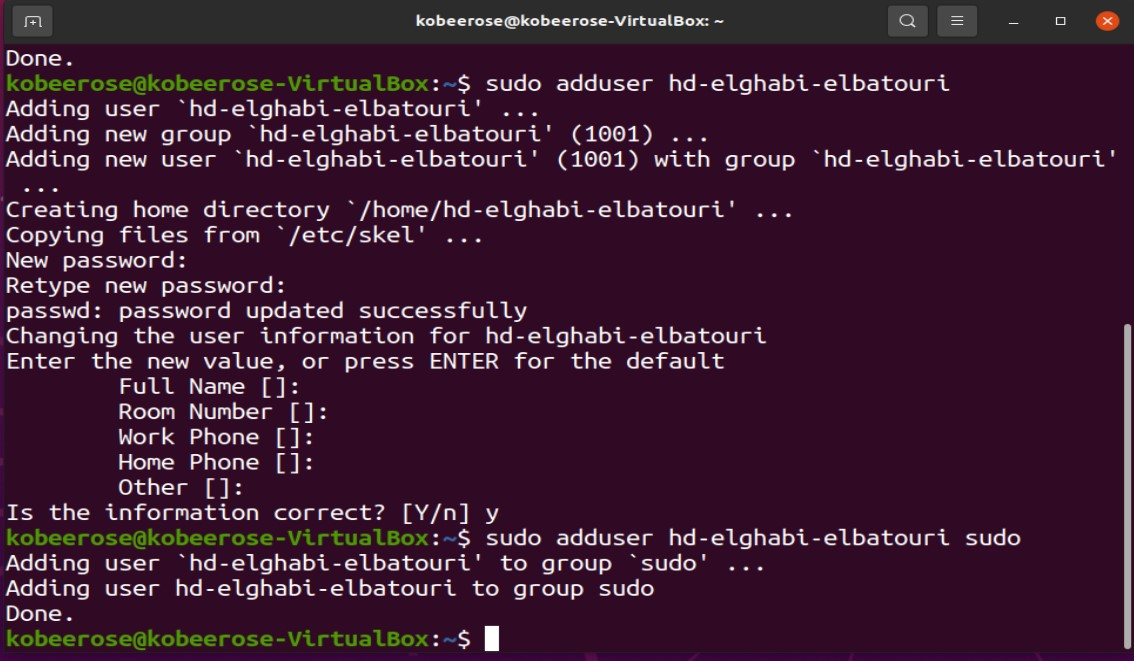
\includegraphics[width=1\linewidth]{Big_Data/Hadoop/Apache Hadoop Installation/Adding new user to sudo group}
\end{center} 
\caption{Adding new user to sudo group} 
\end{figure} 
\FloatBarrier



\par Downloadning Hadoop, Java Development Kit, code_java.zip ( the java source code of the MapReduce "word count" program ), "classpath" script used to set up the variables of the compilation environment, and finally The poeme.txt file to used for manipulations.
\\
\begin{figure}[!htb] 
\begin{center} 
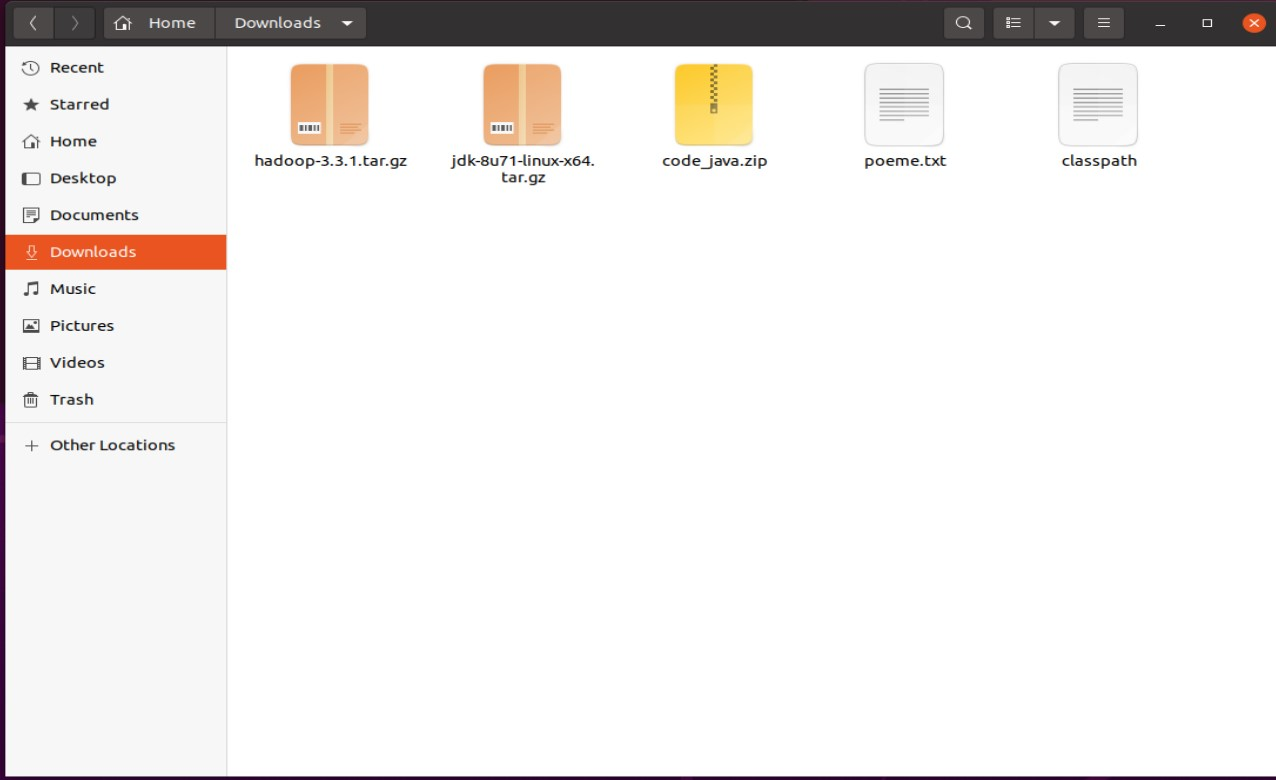
\includegraphics[width=1\linewidth]{Big_Data/Hadoop/Apache Hadoop Installation/Downloading required files} 
\end{center} 
\caption{Downloading required files} 
\end{figure} 
\FloatBarrier

\section{Setting up the ssh key }

\par Install the necessary "openssh-server" package for ssh.
\\
\begin{figure}[!htb] 
\begin{center} 
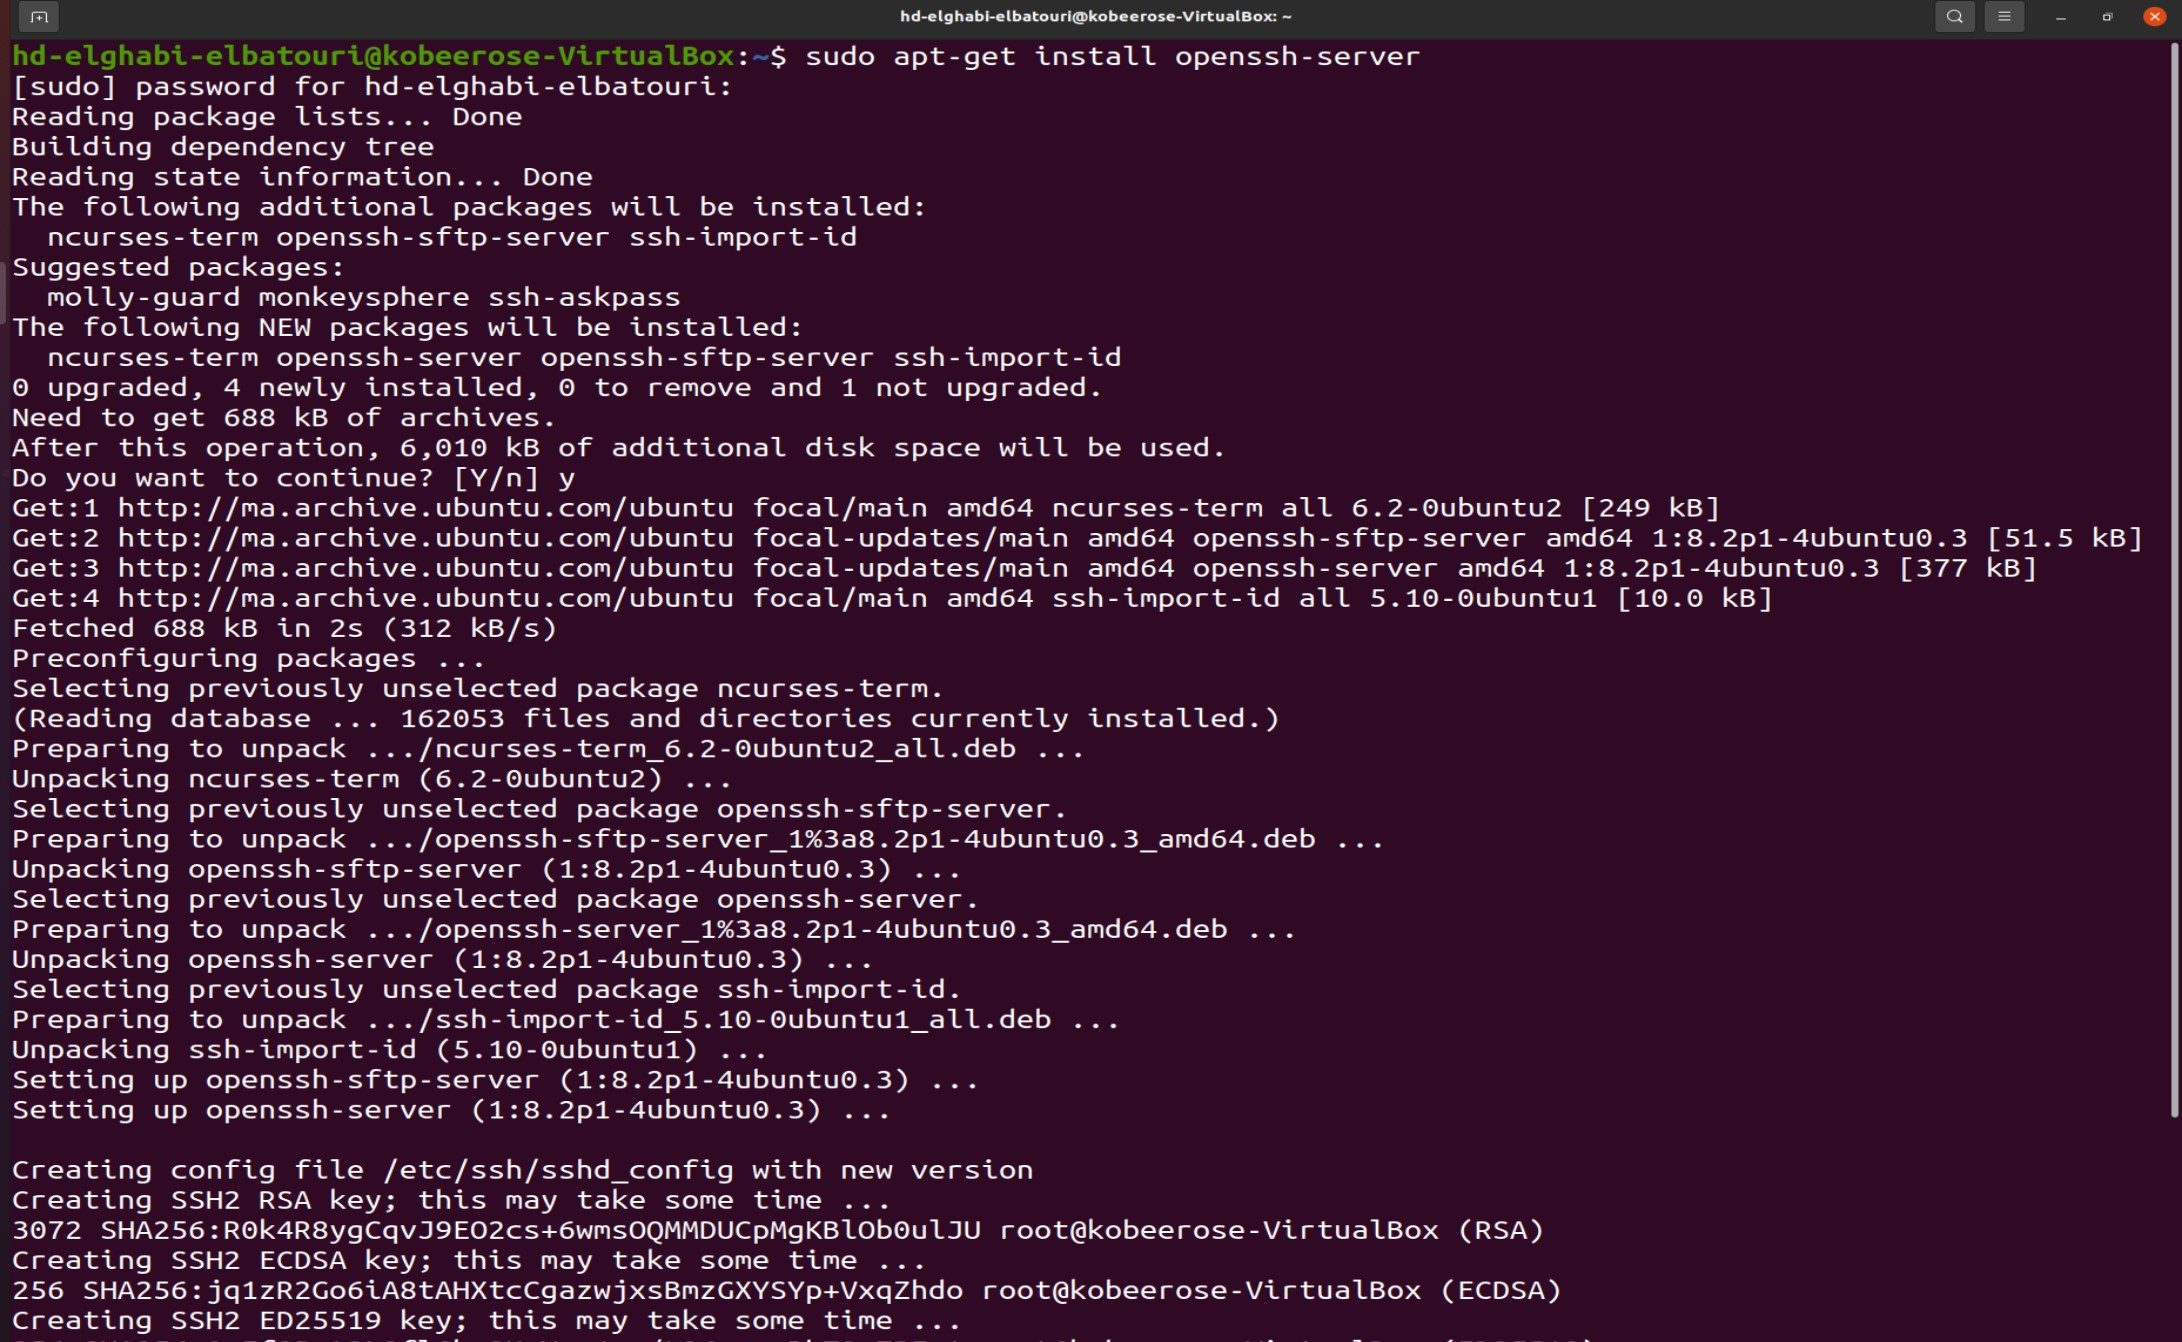
\includegraphics[width=1\linewidth]{Big_Data/Hadoop/Apache Hadoop Installation/Installing openssh-server} 
\end{center} 
\caption{Installing openssh-server} 
\end{figure} 
\FloatBarrier



\par Now you have to set up the ssh key for your own account.
\\
\begin{figure}[!htb] 
\begin{center} 
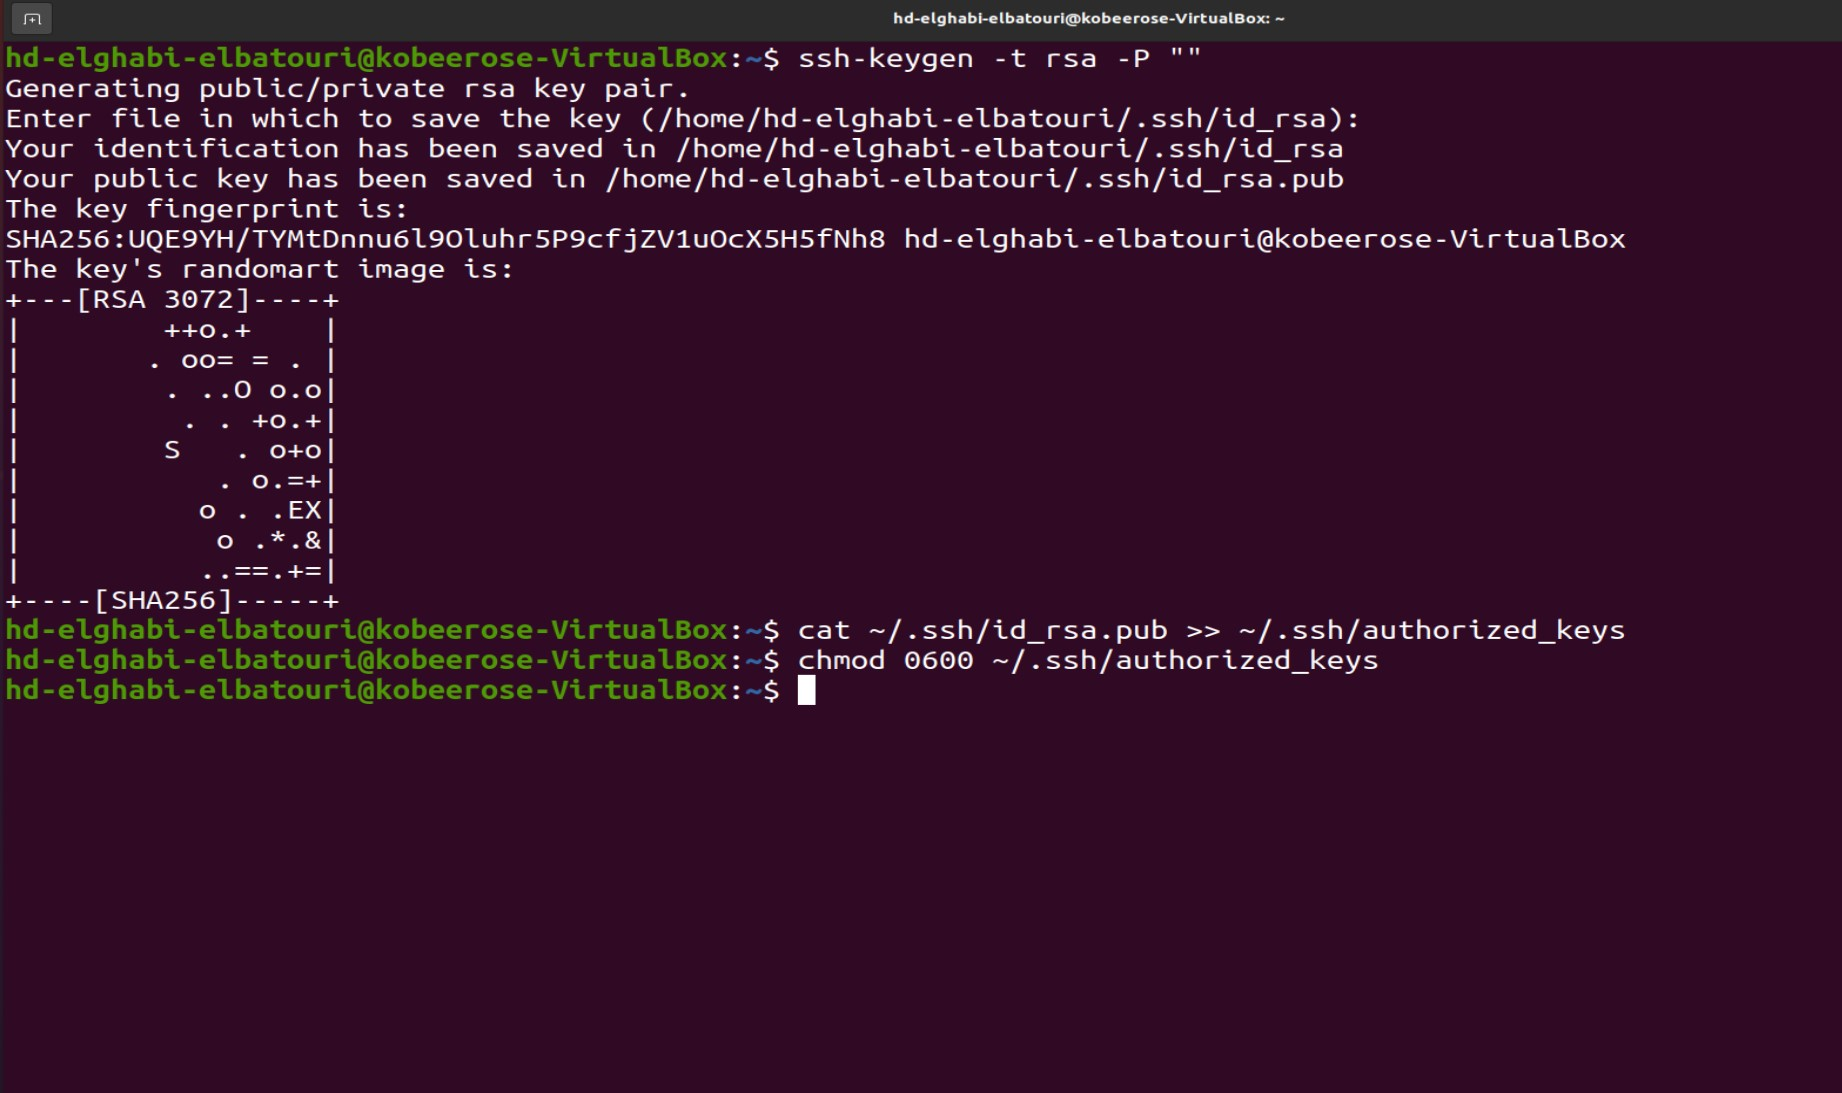
\includegraphics[width=1\linewidth]{Big_Data/Hadoop/Apache Hadoop Installation/Creating SSH key} 
\end{center} 
\caption{Creating SSH key} 
\end{figure} 
\FloatBarrier

\section{Section_name}

\par we Copy the public key to the localhost server.
\\
\begin{figure}[!htb] 
\begin{center} 
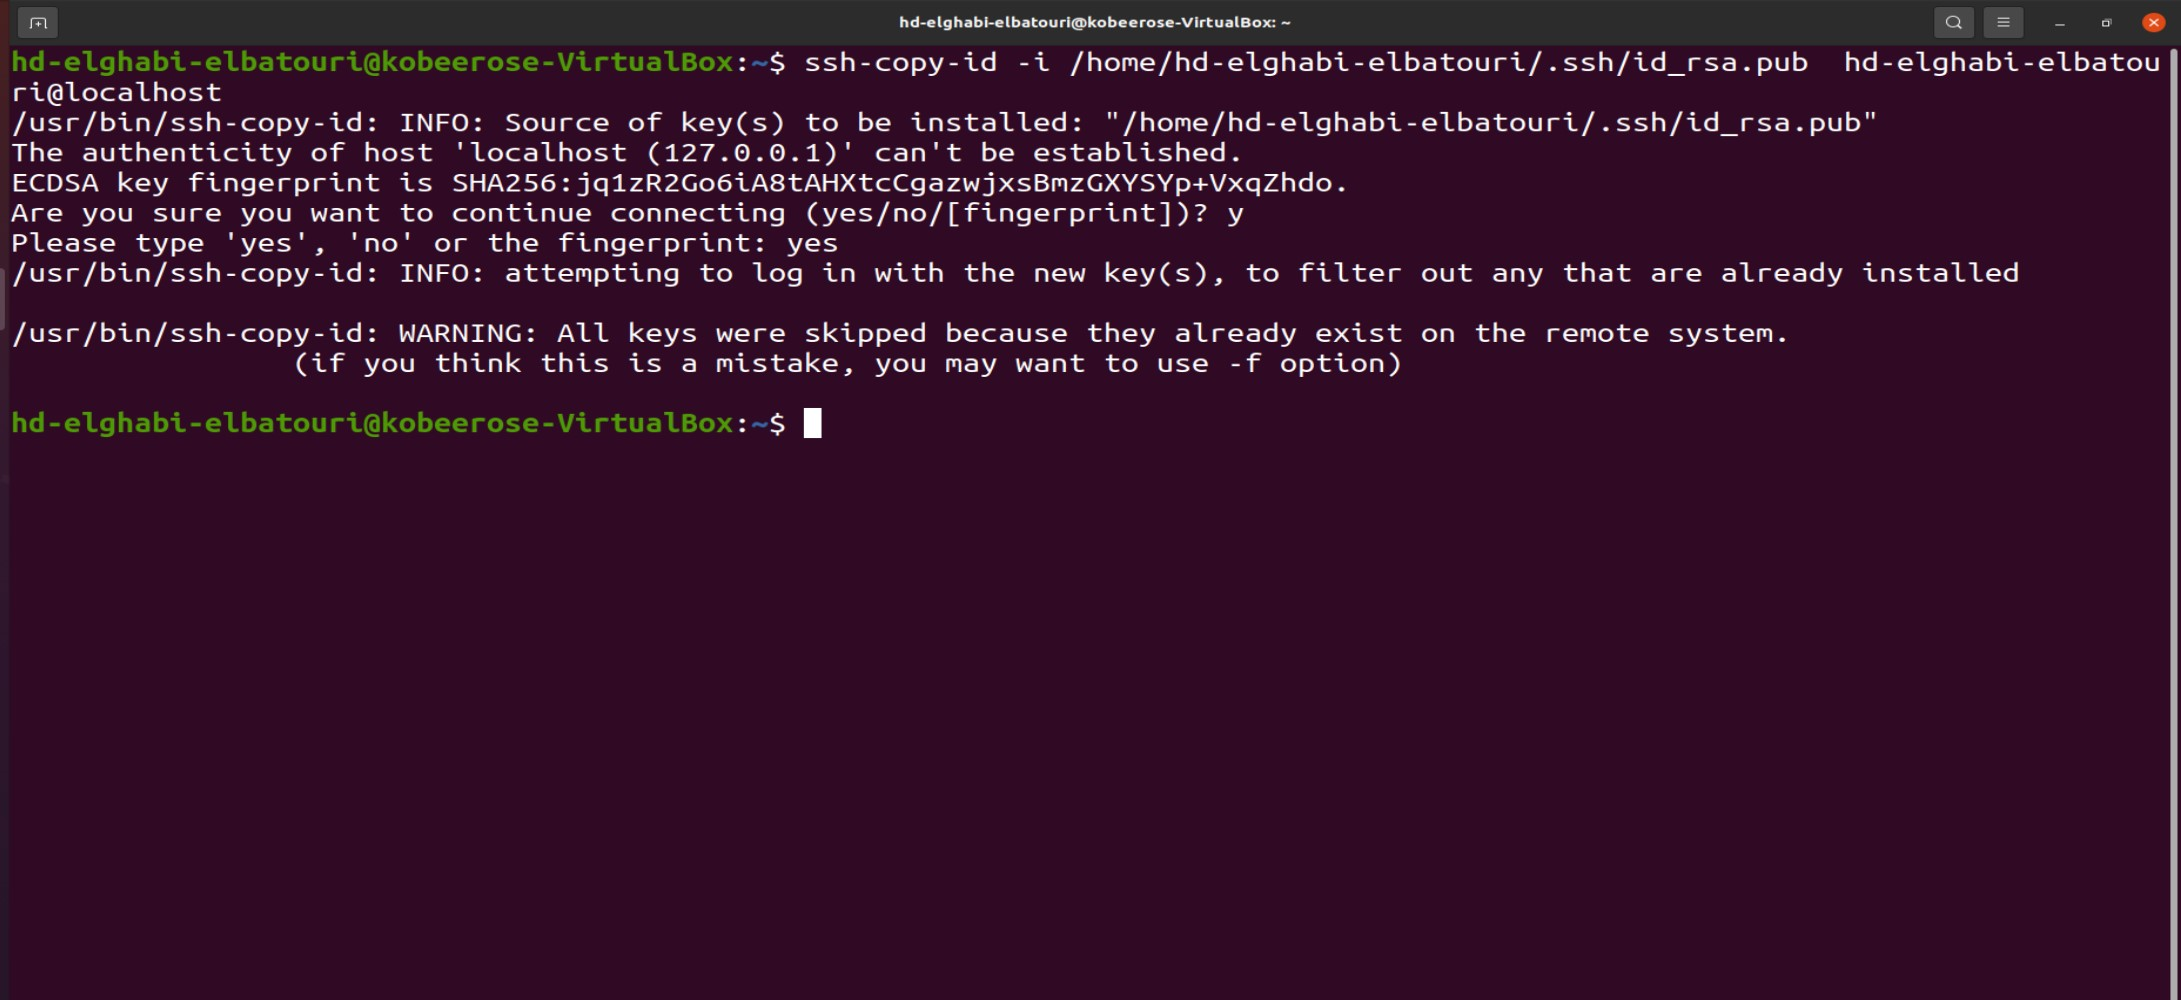
\includegraphics[width=1\linewidth]{Big_Data/Hadoop/Apache Hadoop Installation/Copying the key} 
\end{center} 
\caption{Copying the key} 
\end{figure} 
\FloatBarrier



\par Let's test the connection to localhost.
\\
\begin{figure}[!htb] 
\begin{center} 
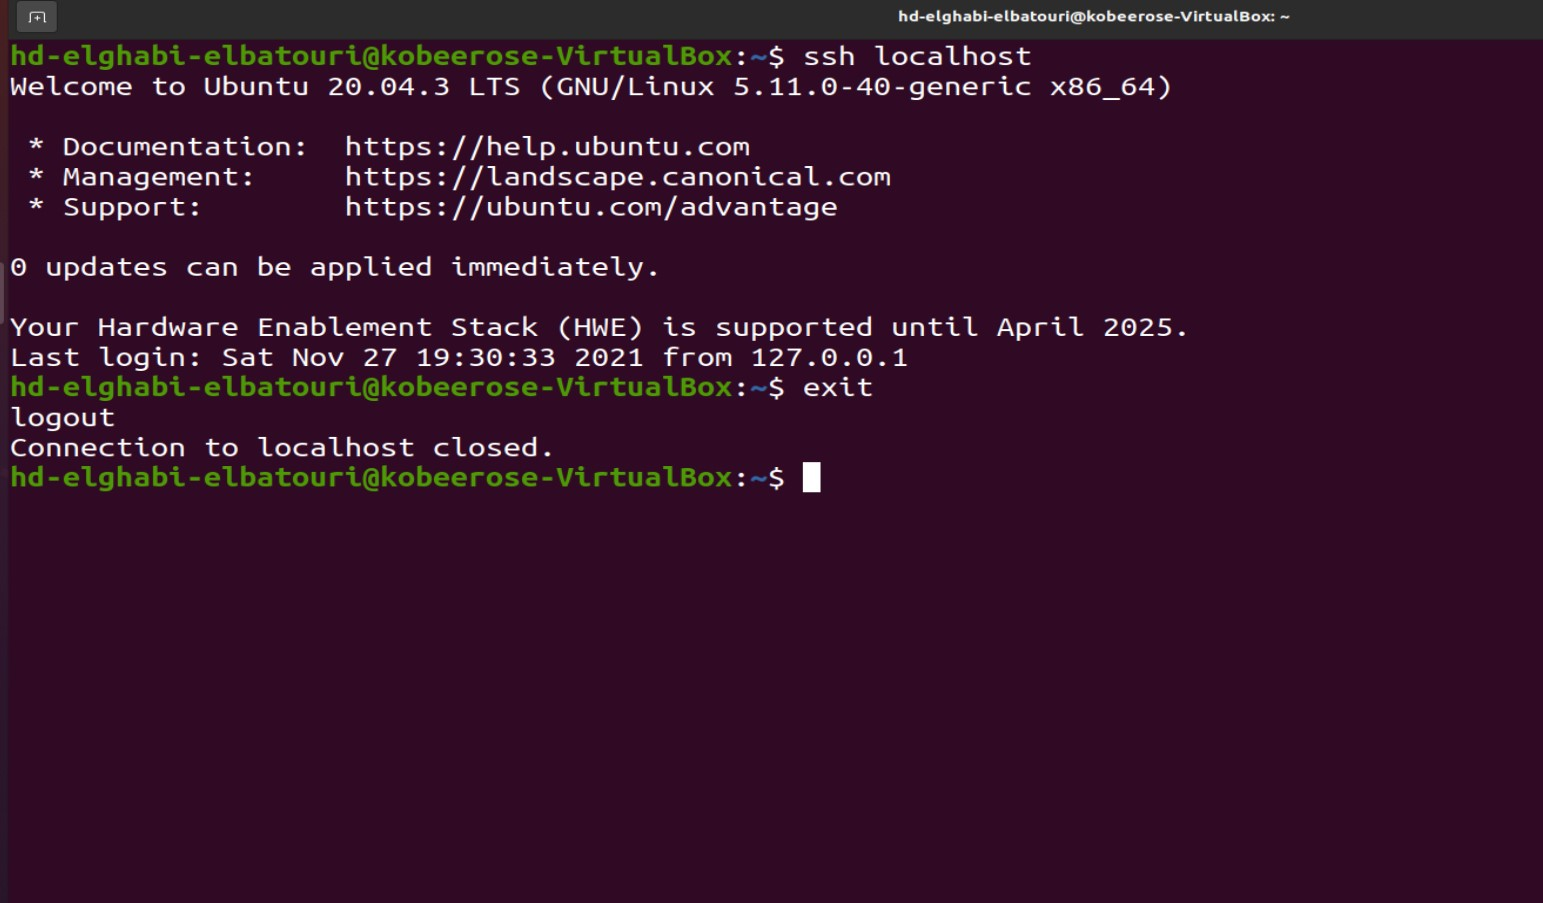
\includegraphics[width=1\linewidth]{Big_Data/Hadoop/Apache Hadoop Installation/Connecting to localhost} 
\end{center} 
\caption{Connecting to localhost} 
\end{figure} 
\FloatBarrier

\section{Installing JAVA 8}

\par We will install in the / opt / java directory to ensure a global access.
\\
\begin{figure}[!htb] 
\begin{center} 
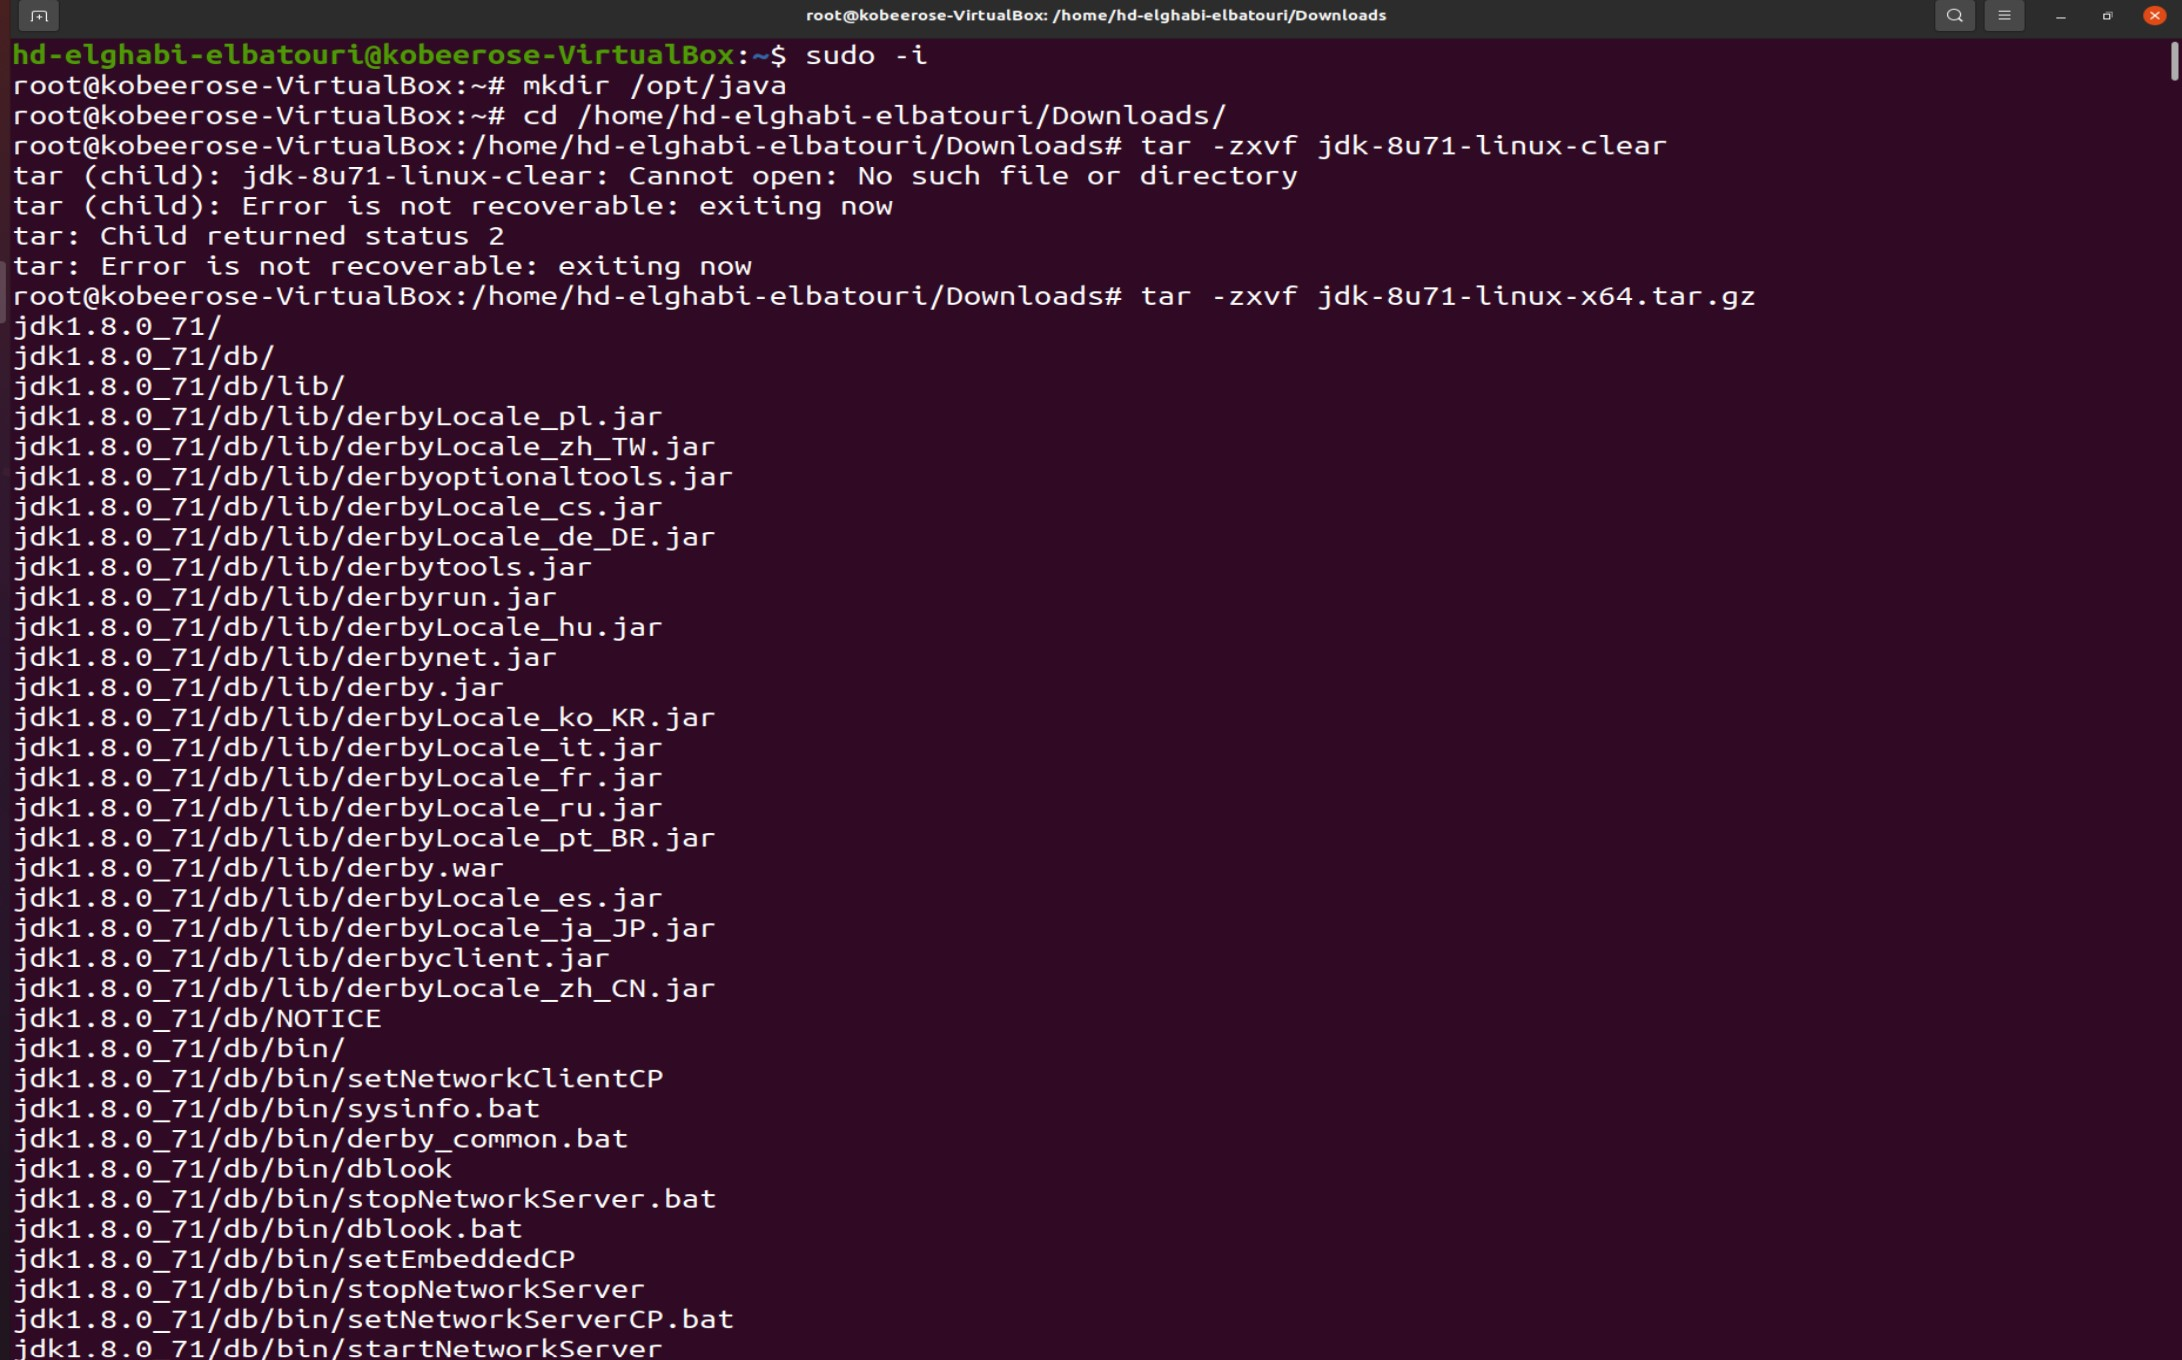
\includegraphics[width=1\linewidth]{Big_Data/Hadoop/Apache Hadoop Installation/Extracting files} 
\end{center} 
\caption{Extracting files} 
\end{figure} 
\FloatBarrier

\begin{figure}[!htb] 
\begin{center} 
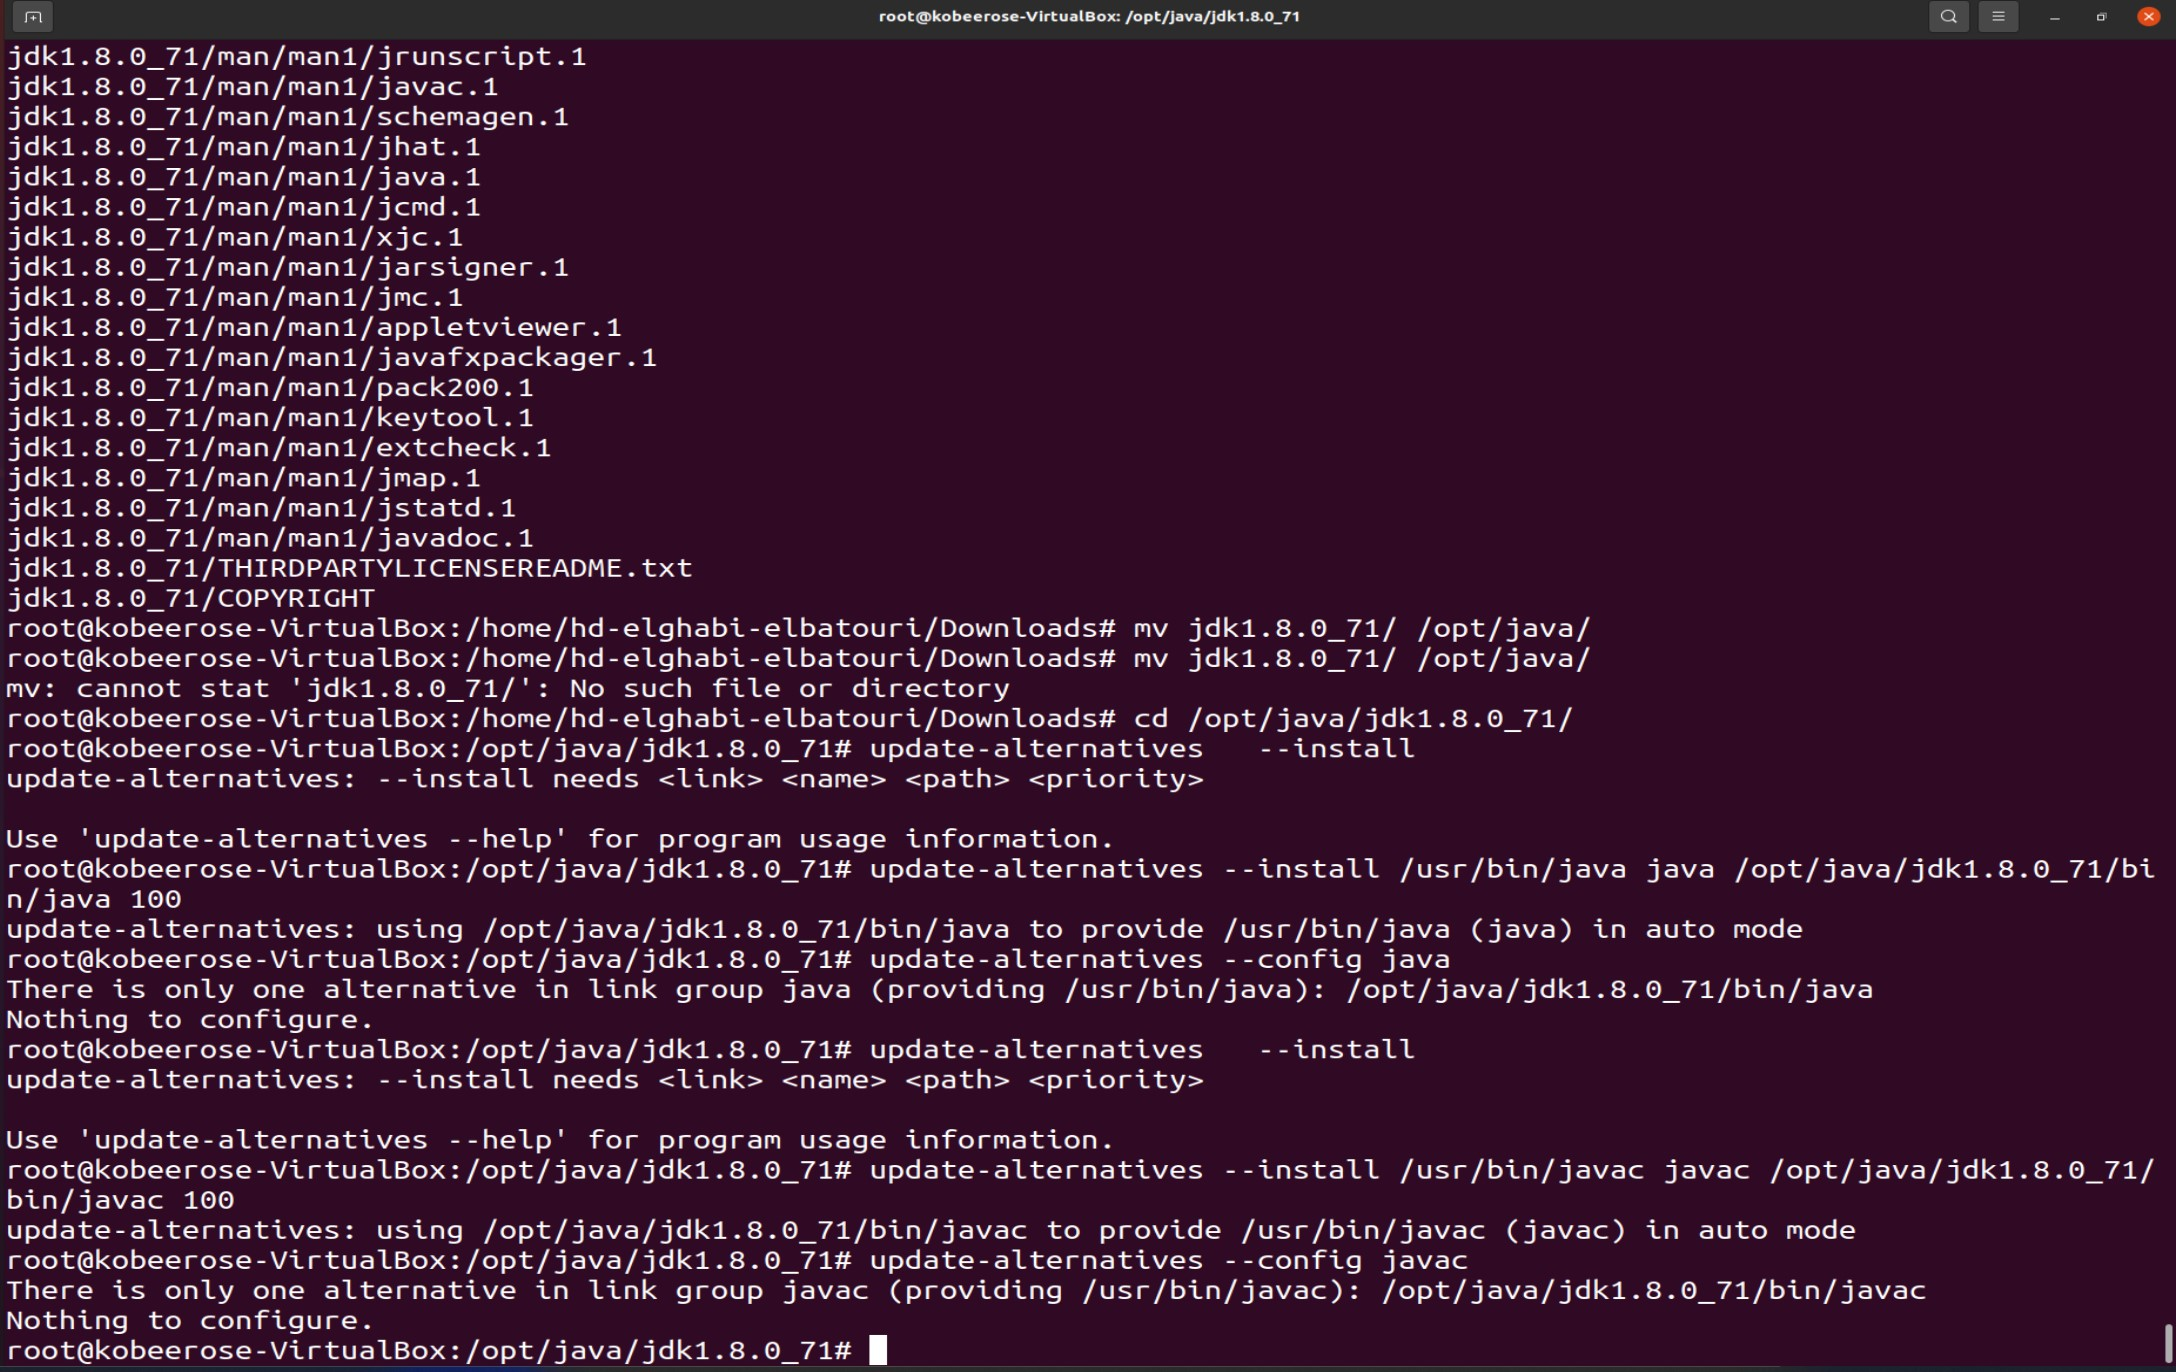
\includegraphics[width=1\linewidth]{Big_Data/Hadoop/Apache Hadoop Installation/Installing java and javac} 
\end{center} 
\caption{Installing java and javac} 
\end{figure} 
\FloatBarrier


\par To permanently set up JAVA environment variables for all users, we will configure profile file.
\\
\begin{figure}[!htb] 
\begin{center} 
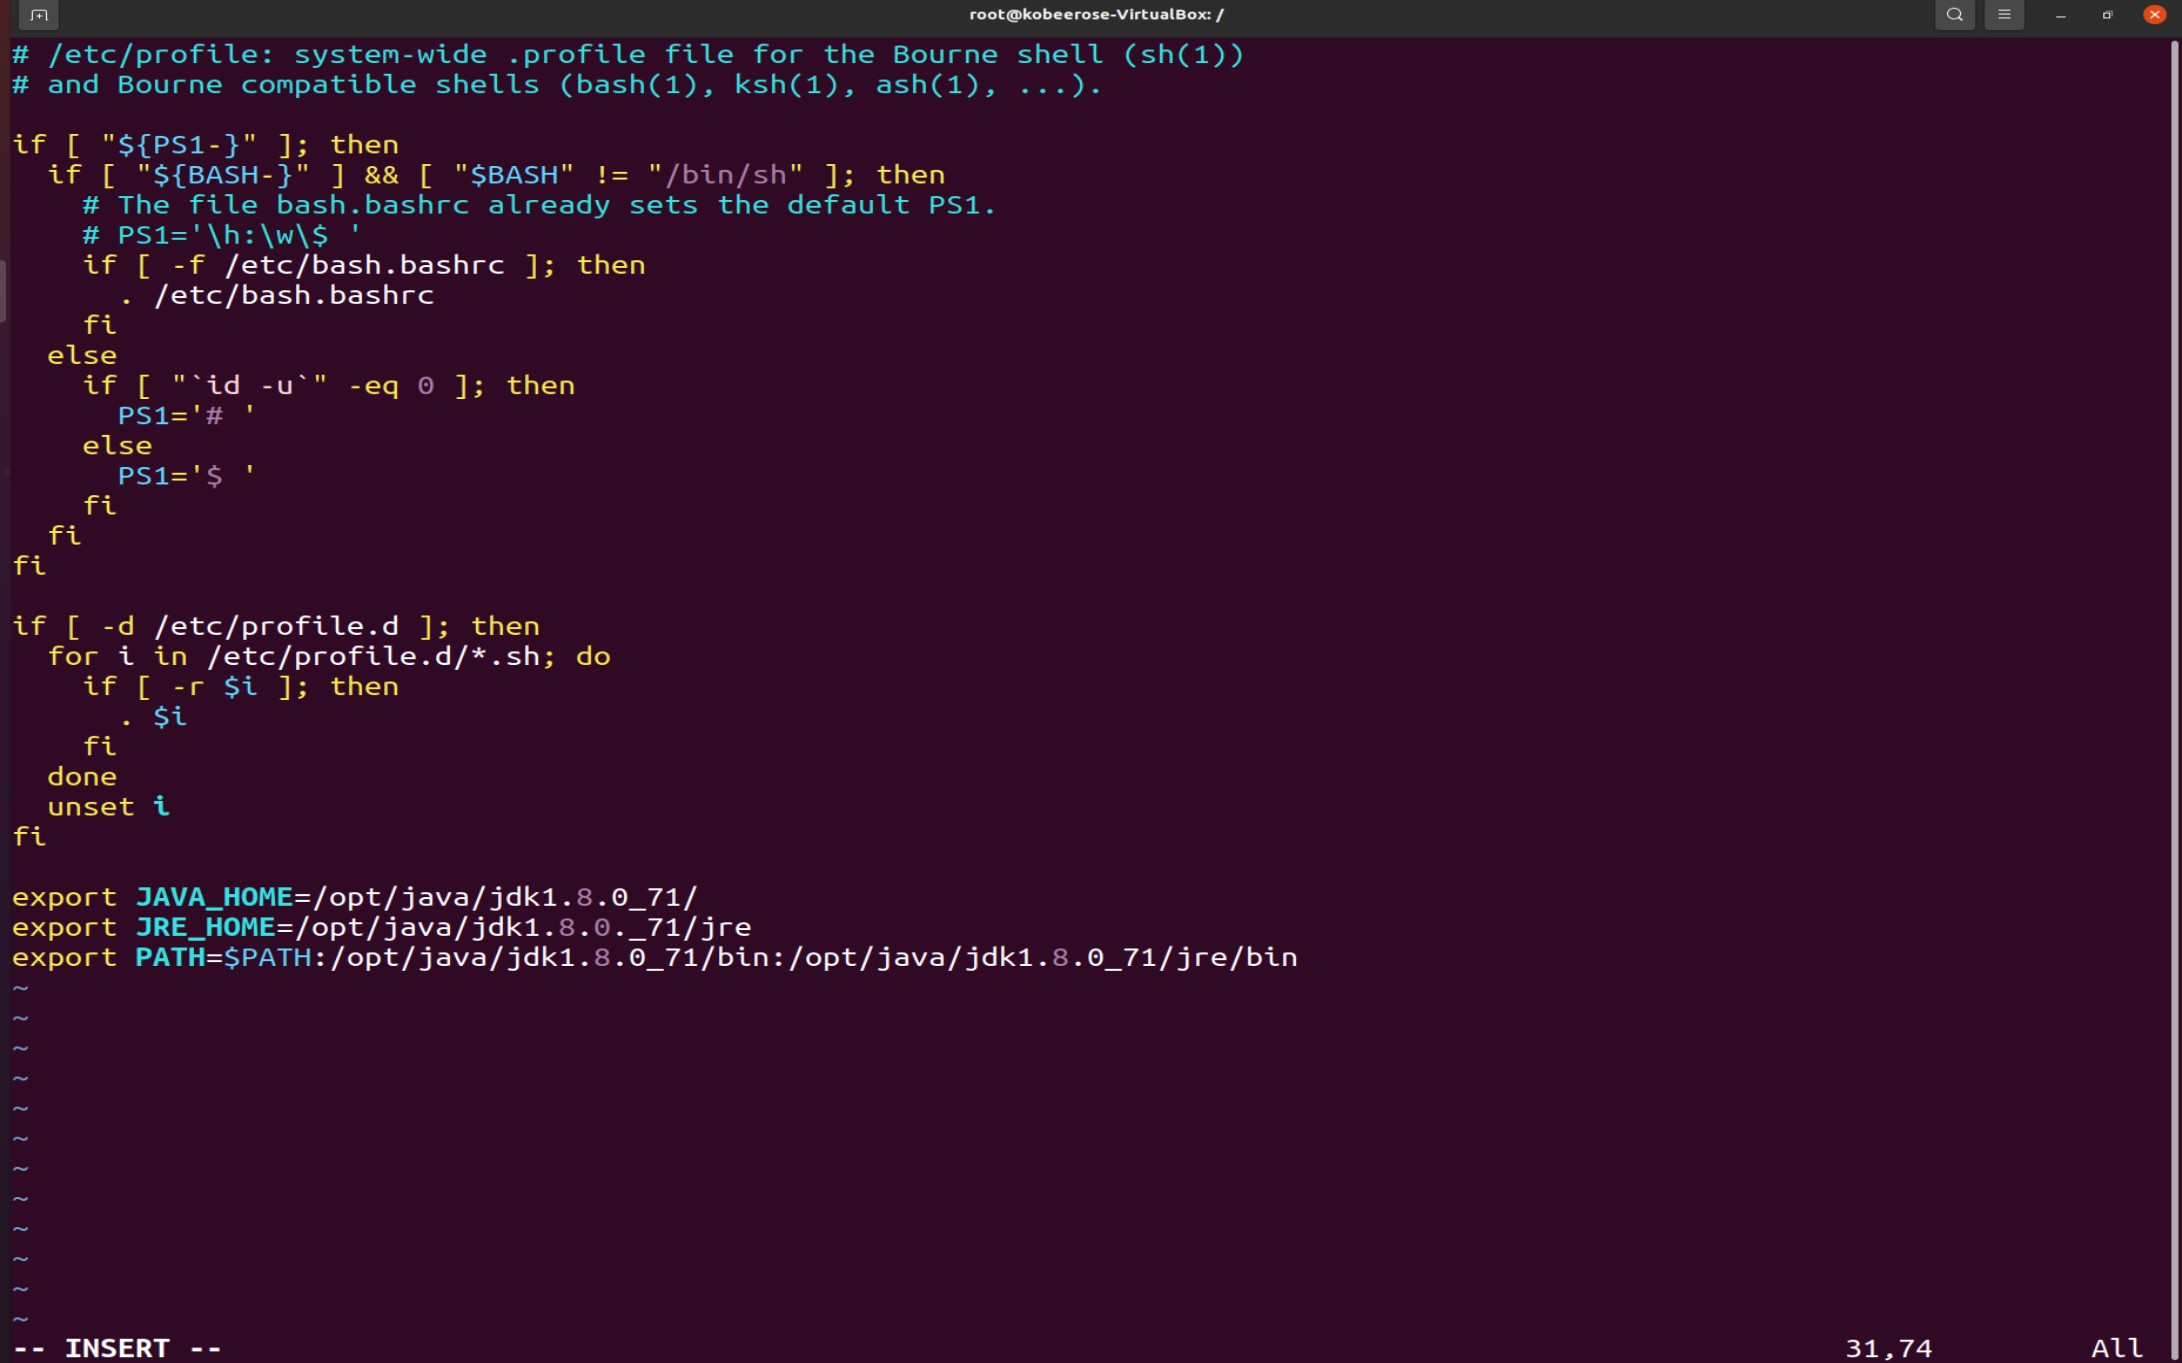
\includegraphics[width=1\linewidth]{Big_Data/Hadoop/Apache Hadoop Installation/profile file config} 
\end{center} 
\caption{profile file config} 
\end{figure} 
\FloatBarrier

\par Le'ts can test the setting of environment variables in the hadoop terminal.
\\
\begin{figure}[!htb] 
\begin{center} 
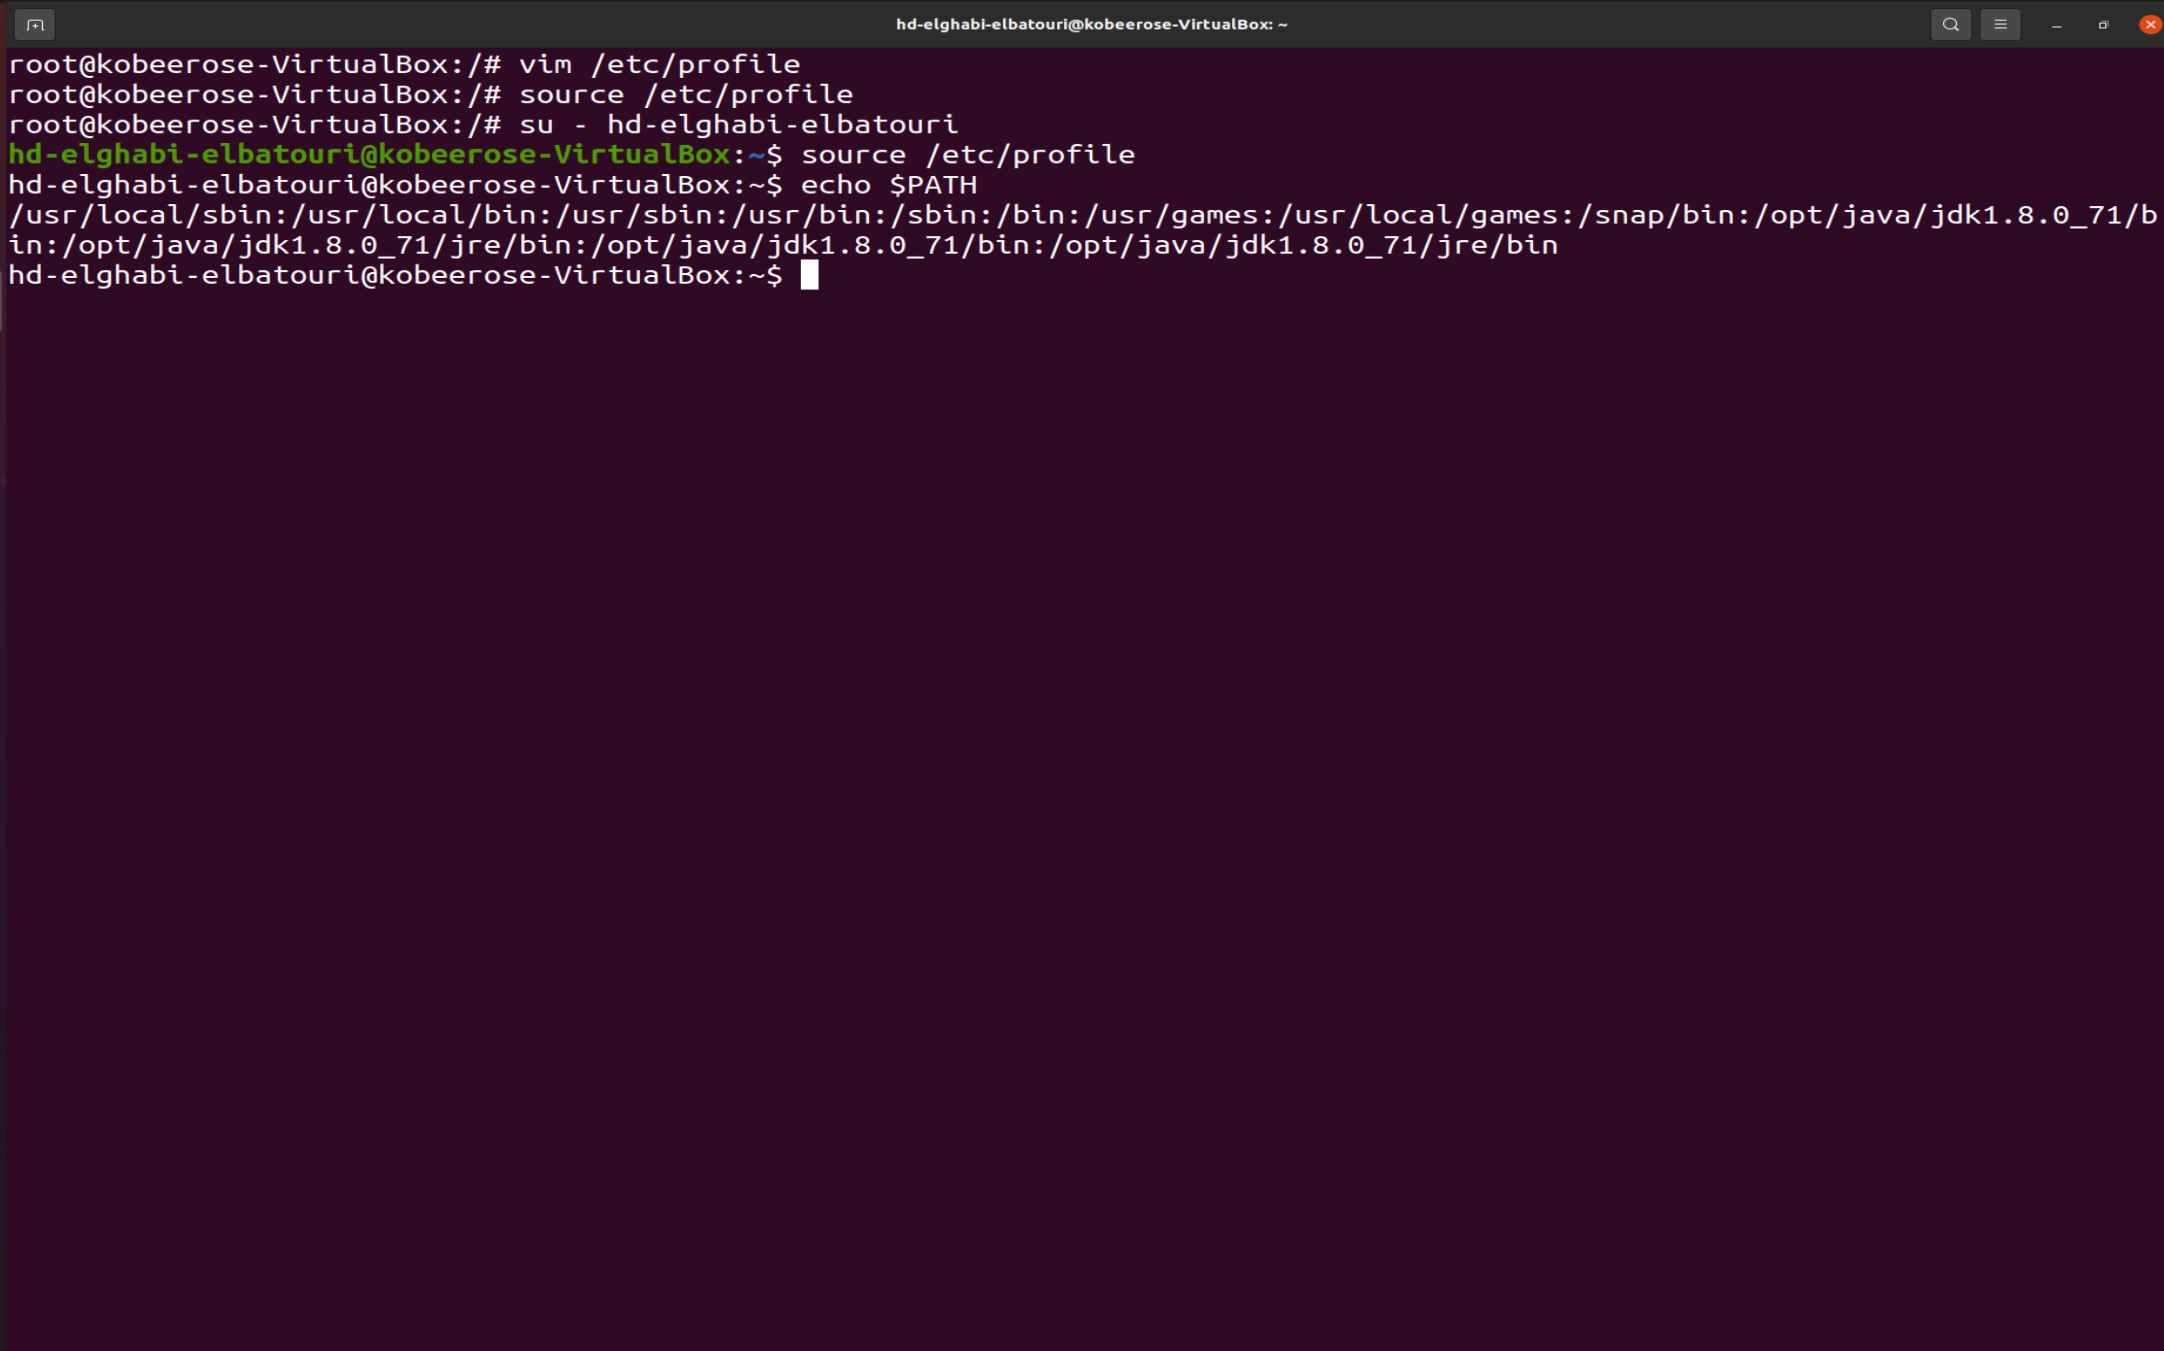
\includegraphics[width=1\linewidth]{Big_Data/Hadoop/Apache Hadoop Installation/Verifying PATH} 
\end{center} 
\caption{Verifying PATH} 
\end{figure} 
\FloatBarrier

\section{Installing Apache Hadoop 3.3.1}

\par Extracting files and Installing Apache Hadoop.
\\
\begin{figure}[!htb] 
\begin{center} 
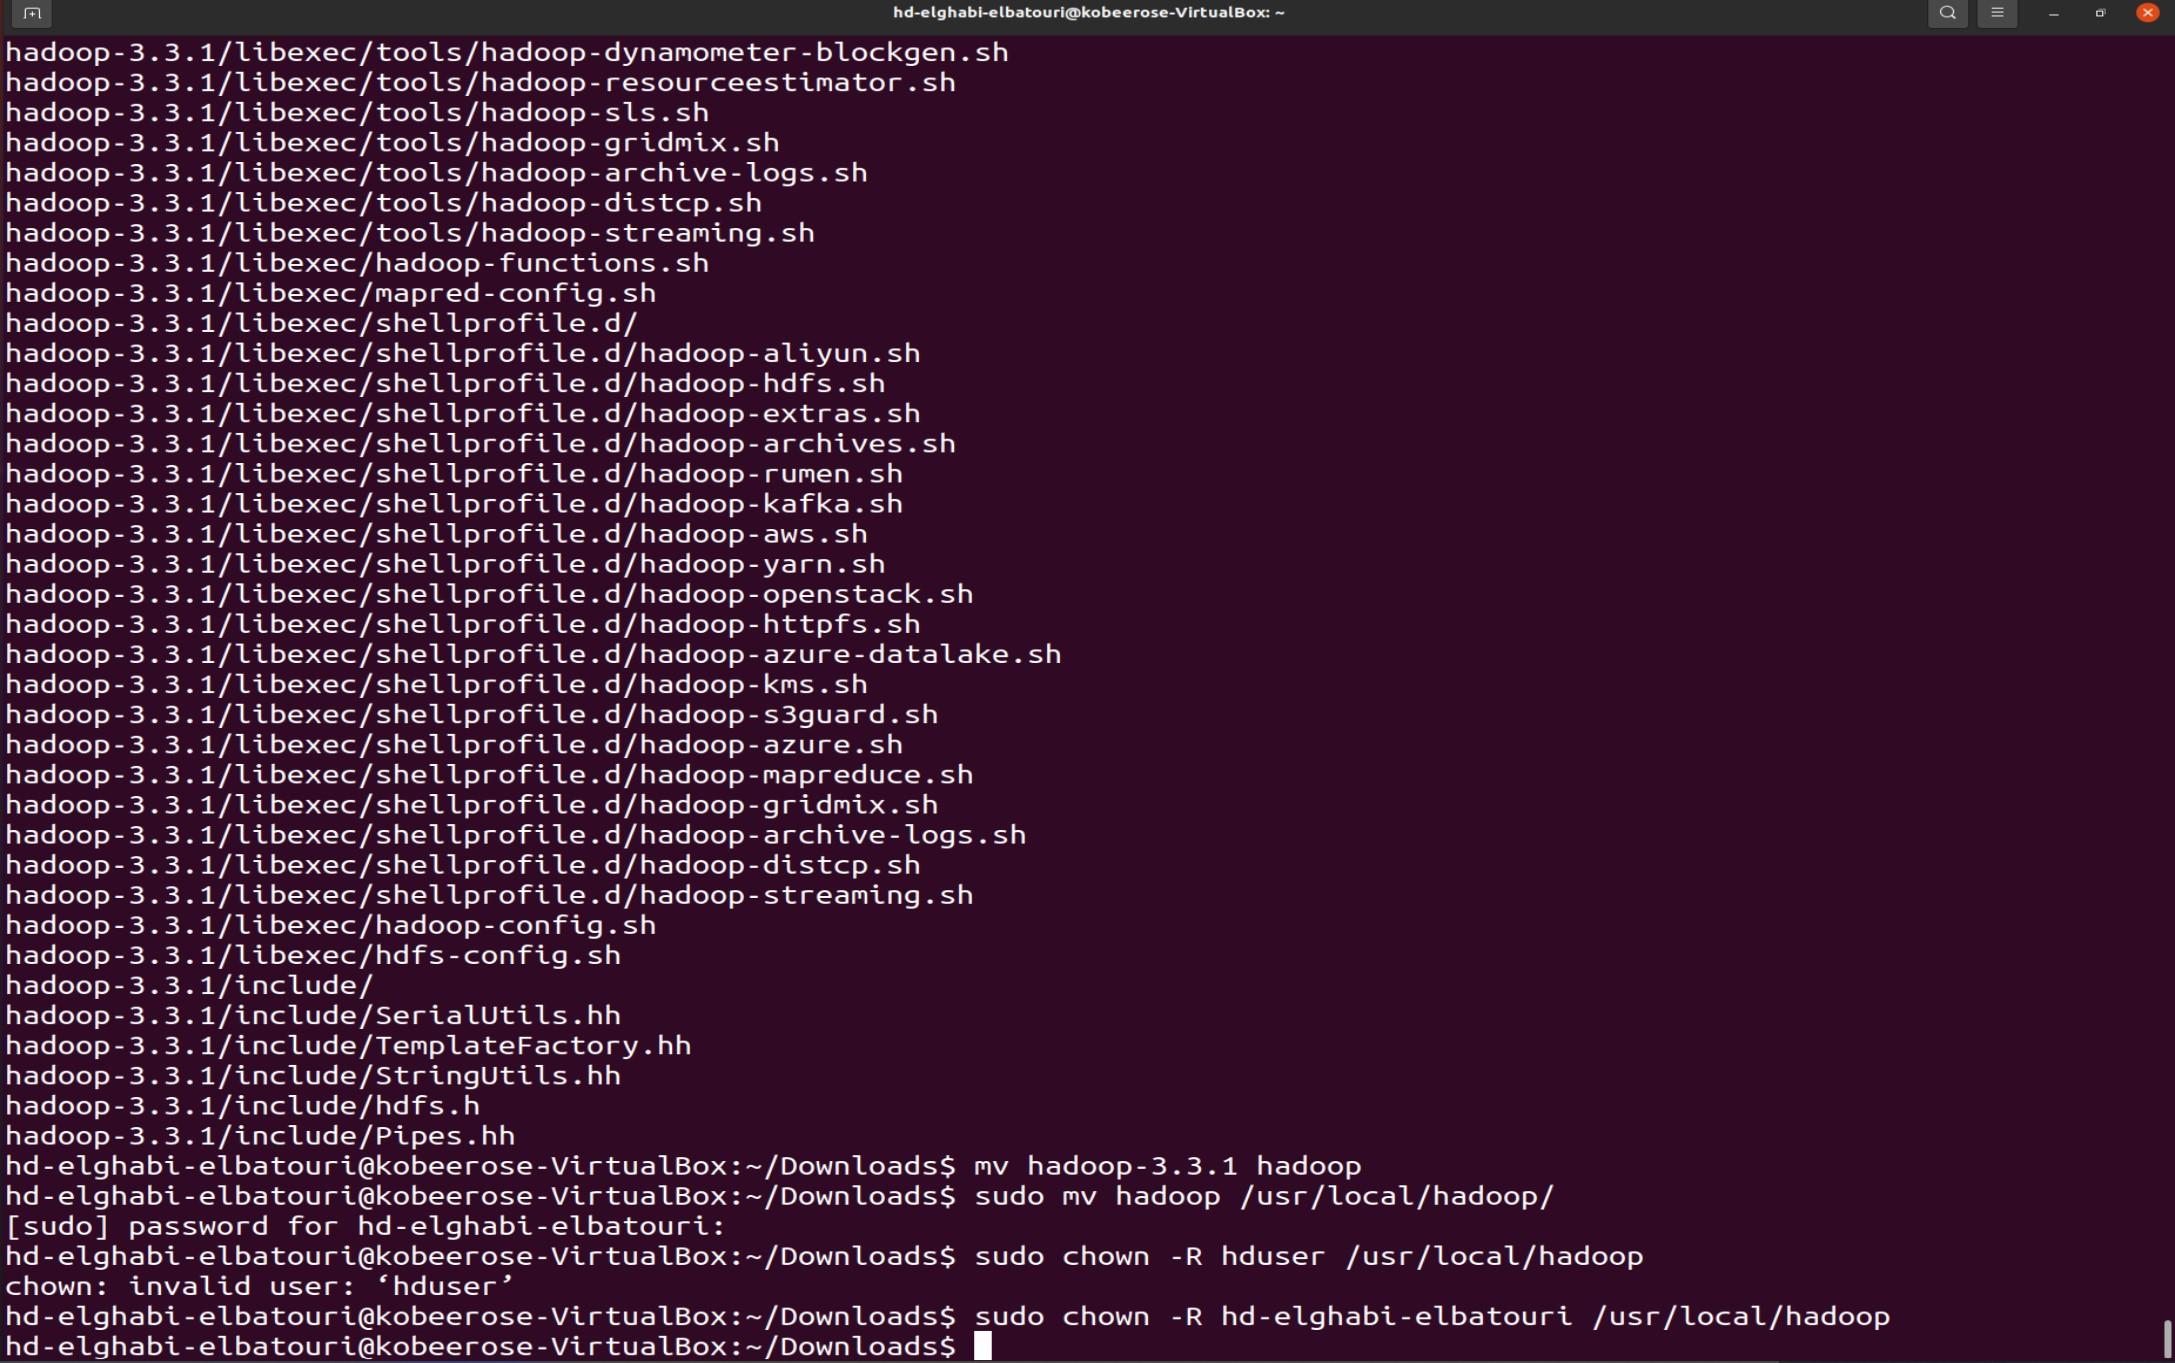
\includegraphics[width=1\linewidth]{Big_Data/Hadoop/Apache Hadoop Installation/Extracting Hadoop}
\end{center} 
\caption{Extracting Hadoop} 
\end{figure} 
\FloatBarrier


\par Create the hadoop data storage directories.
\\
\begin{figure}[!htb] 
\begin{center} 
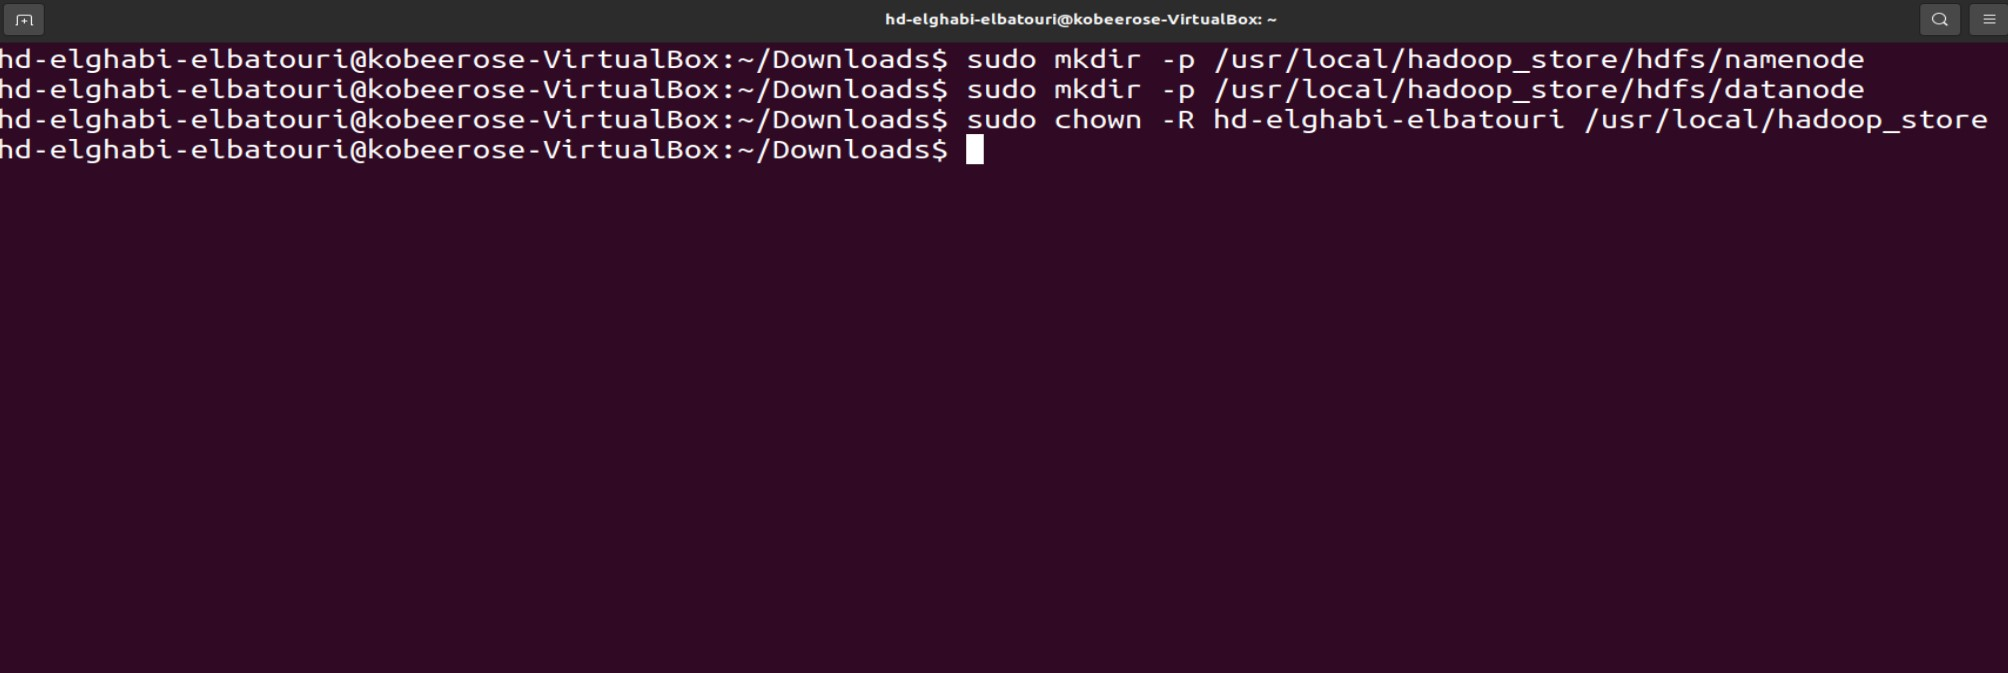
\includegraphics[width=1\linewidth]{Big_Data/Hadoop/Apache Hadoop Installation/Creating Storage repo} 
\end{center} 
\caption{Creating Storage repo} 
\end{figure} 
\FloatBarrier

\section{Configuring Apache Hadoop 3.3.1 }

\par Setting up environment variables for Hadoop.
\\
\begin{figure}[!htb] 
\begin{center} 
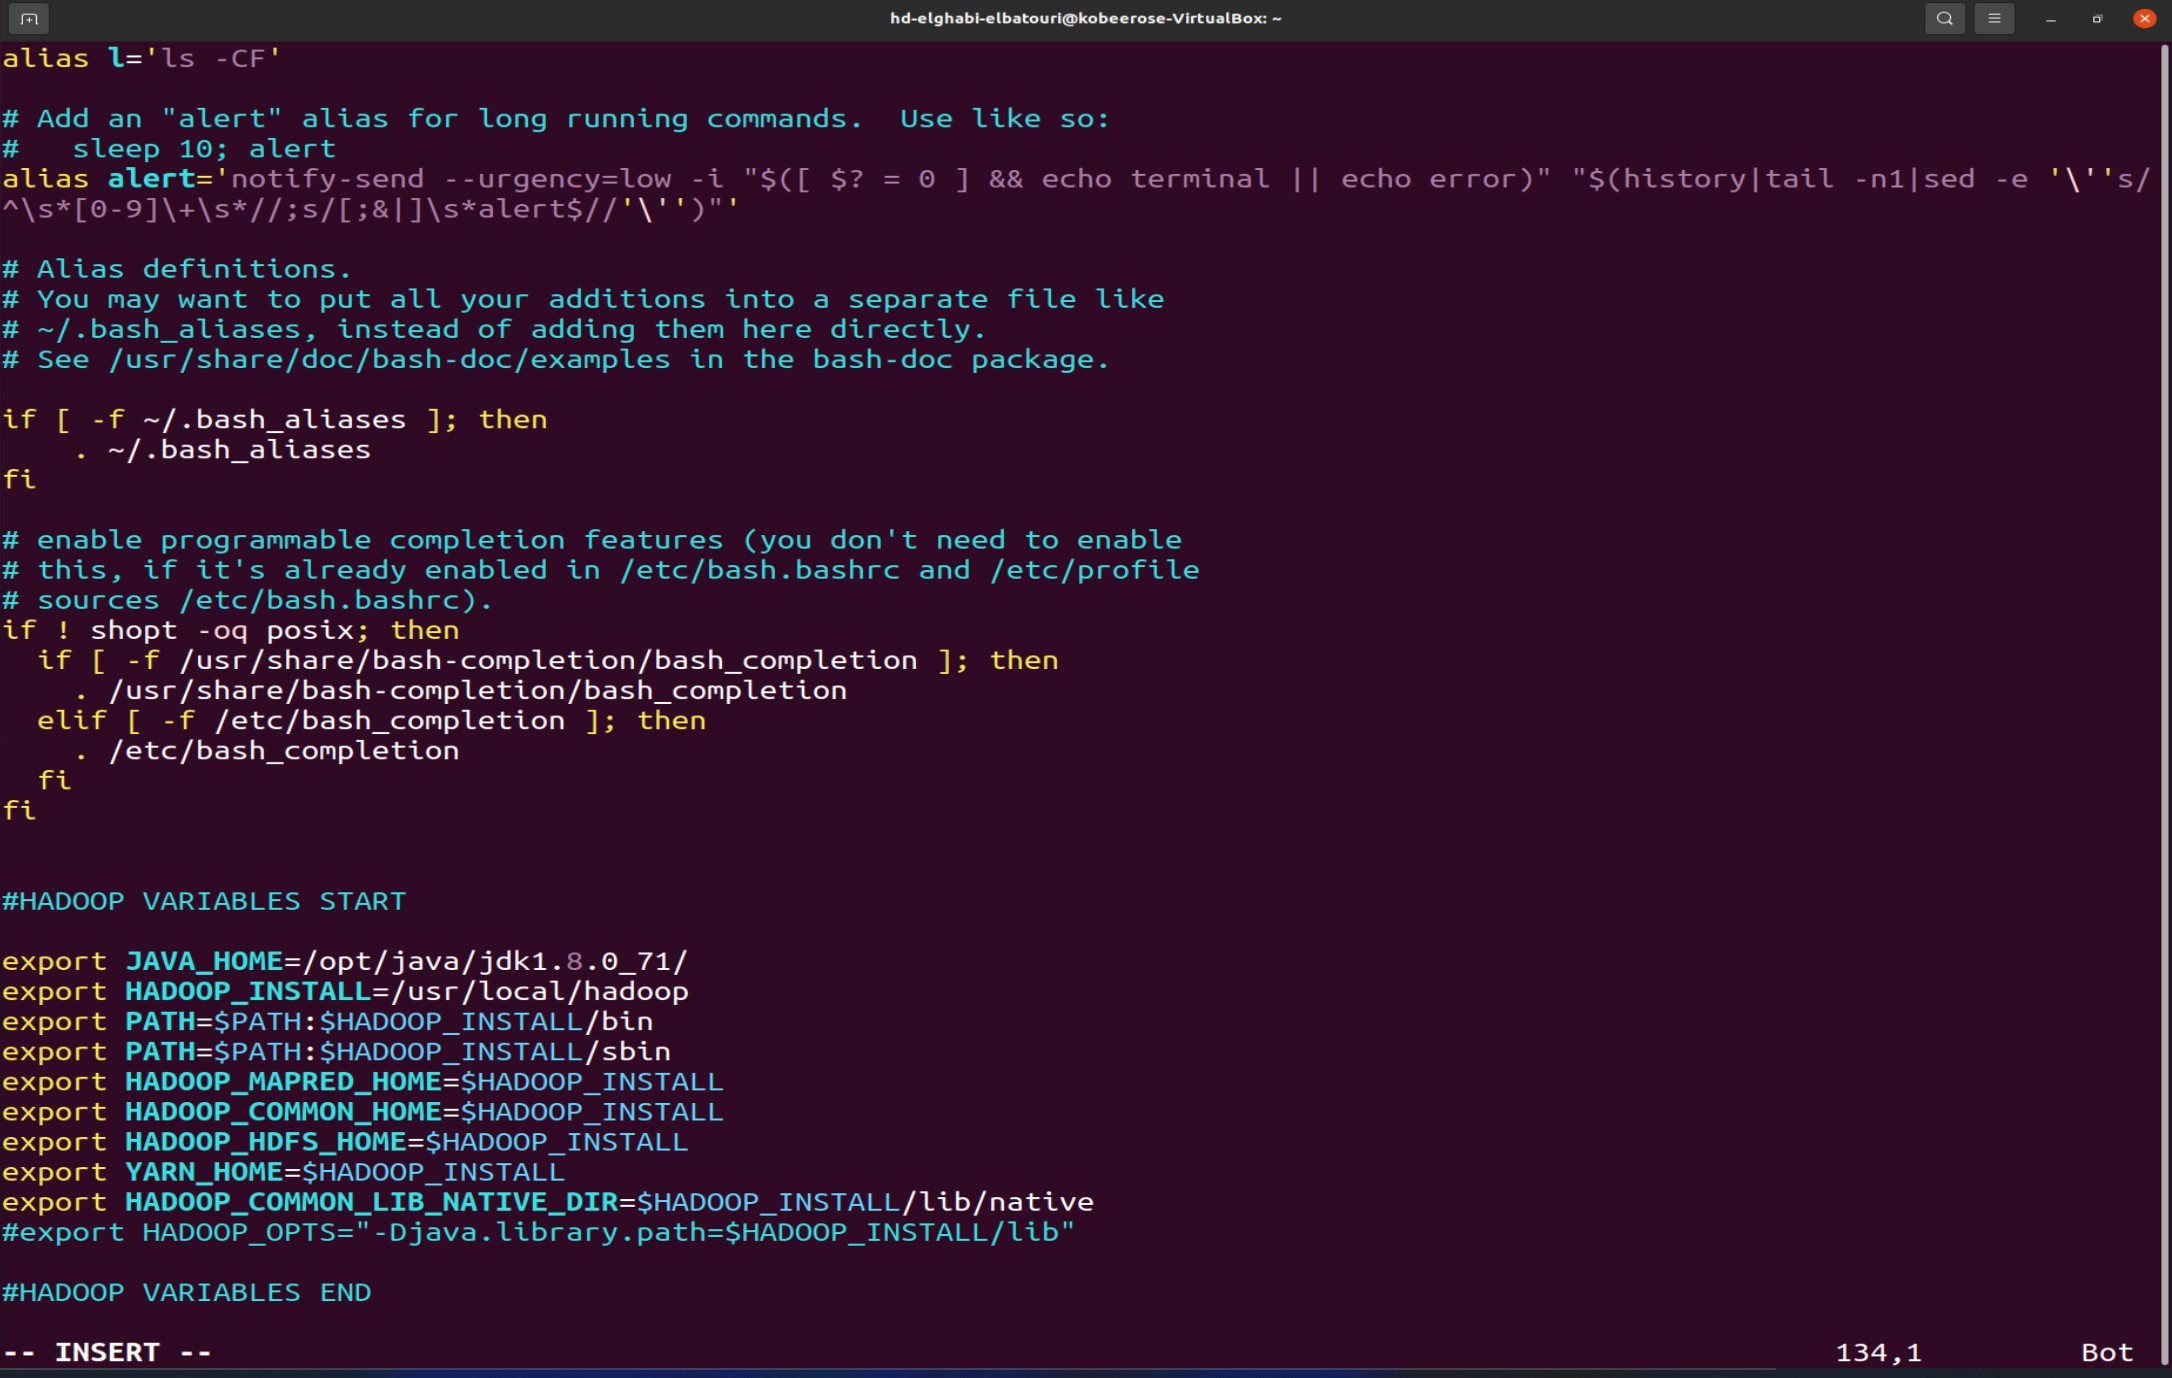
\includegraphics[width=1\linewidth]{Big_Data/Hadoop/Apache Hadoop Installation/Modifying .bashrc file} 
\end{center} 
\caption{Modifying .bashrc file} 
\end{figure} 
\FloatBarrier

\par Editing Hadoop Configuration Files: core-site.xml, hdfs-site.xml, mapred-site.xml, yarn-site.xml then Formatting of the Namenode. 
\\
\begin{figure}[!htb] 
\begin{center} 
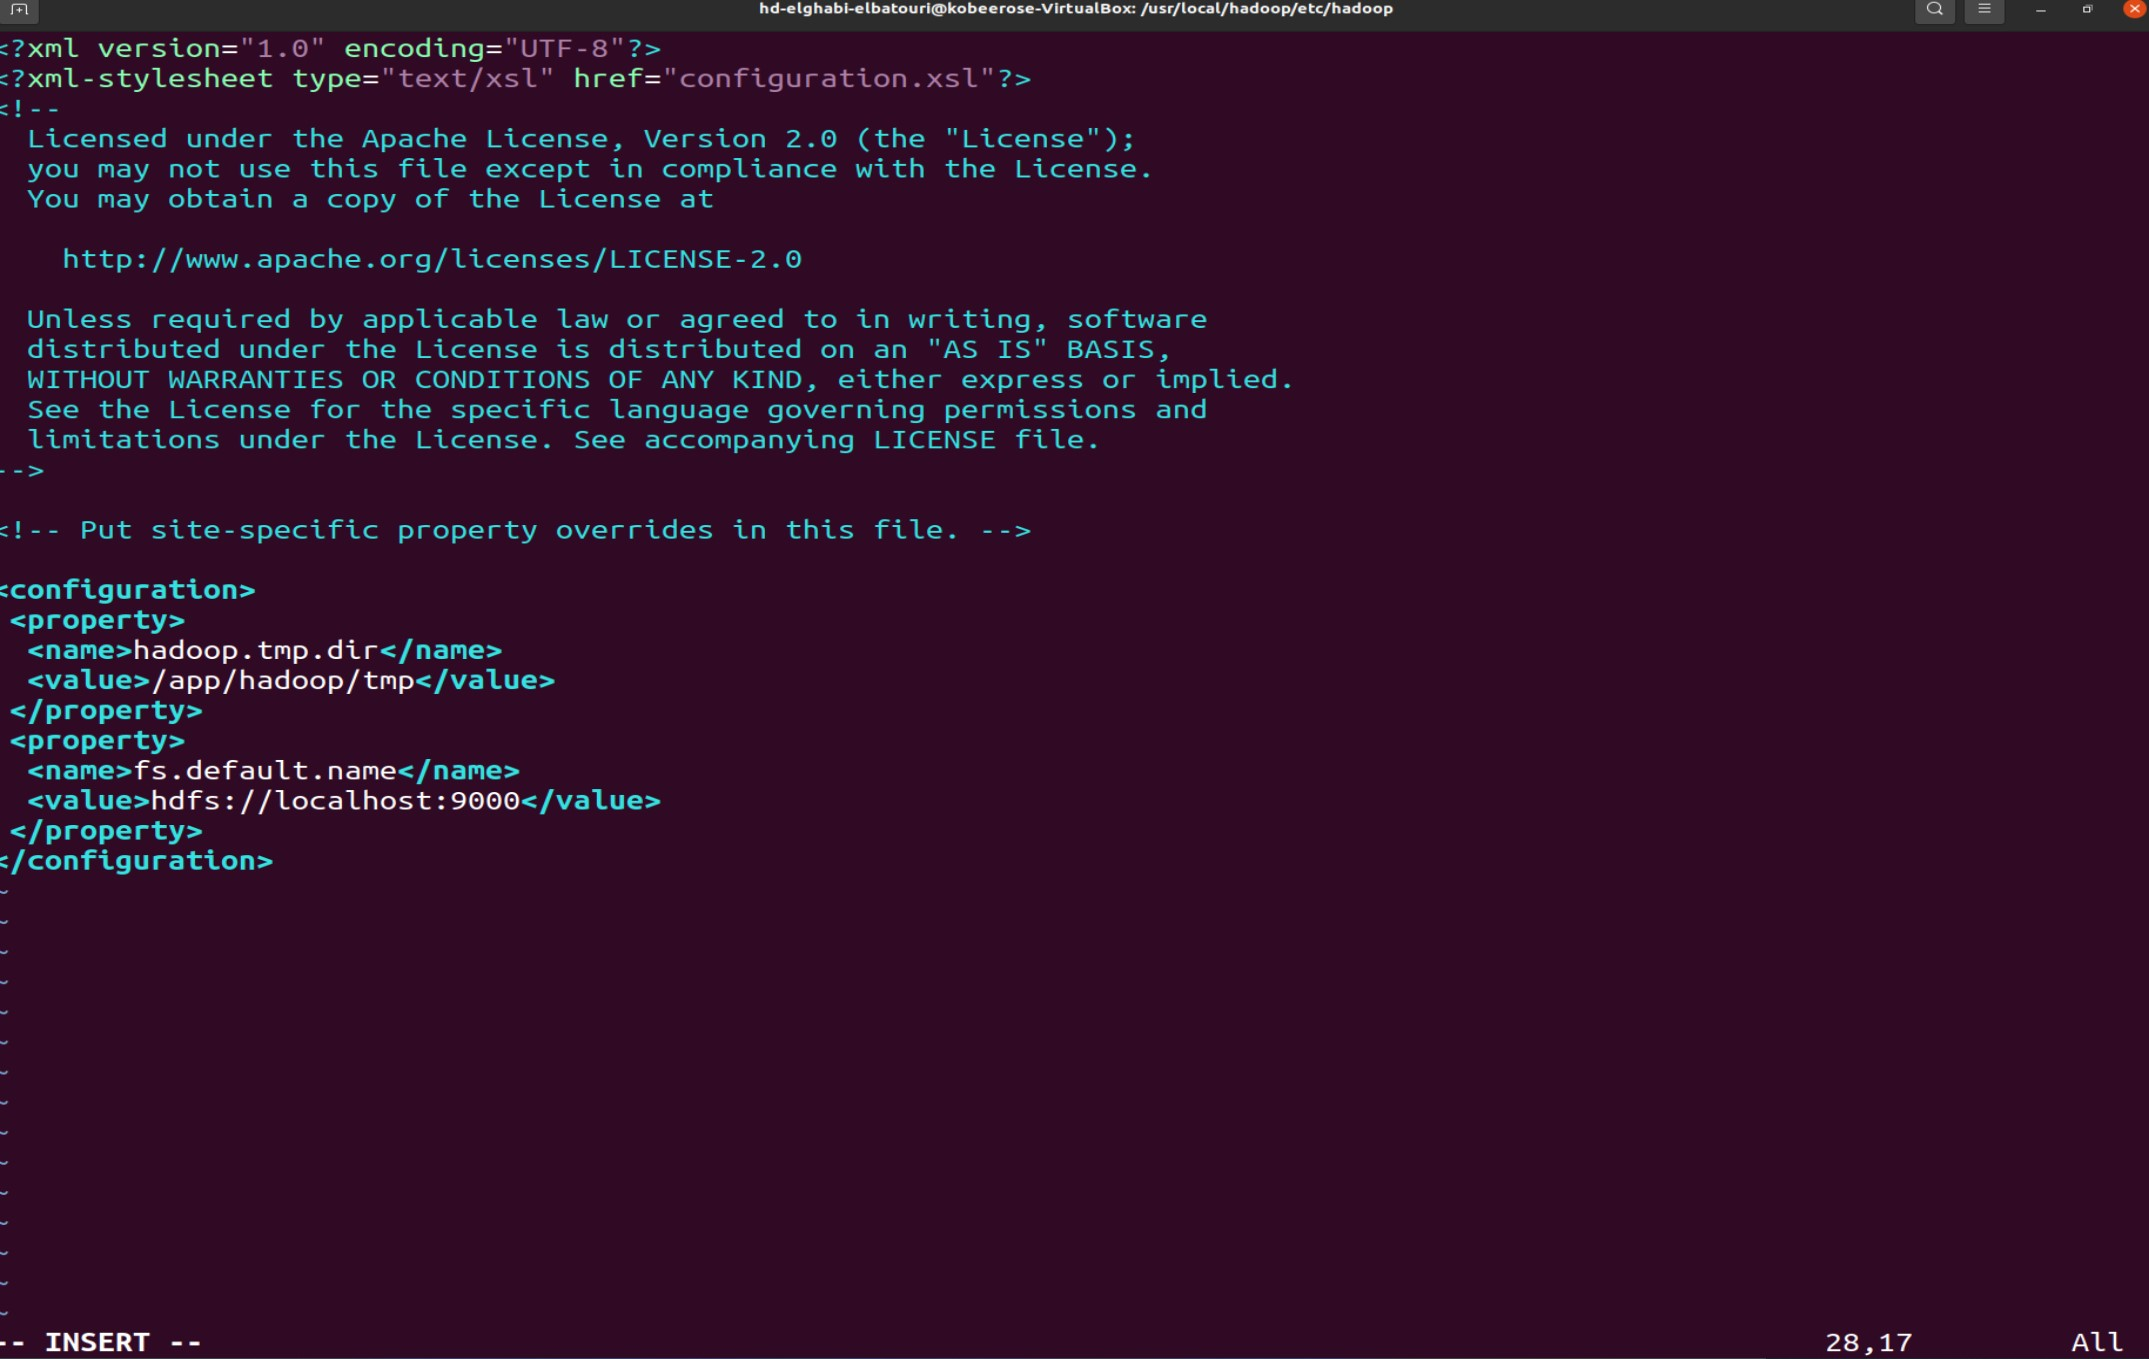
\includegraphics[width=1\linewidth]{Big_Data/Hadoop/Apache Hadoop Installation/core-site.xml config} 
\end{center} 
\caption{core-site.xml config} 
\end{figure} 
\FloatBarrier
\begin{figure}[!htb] 
\begin{center} 
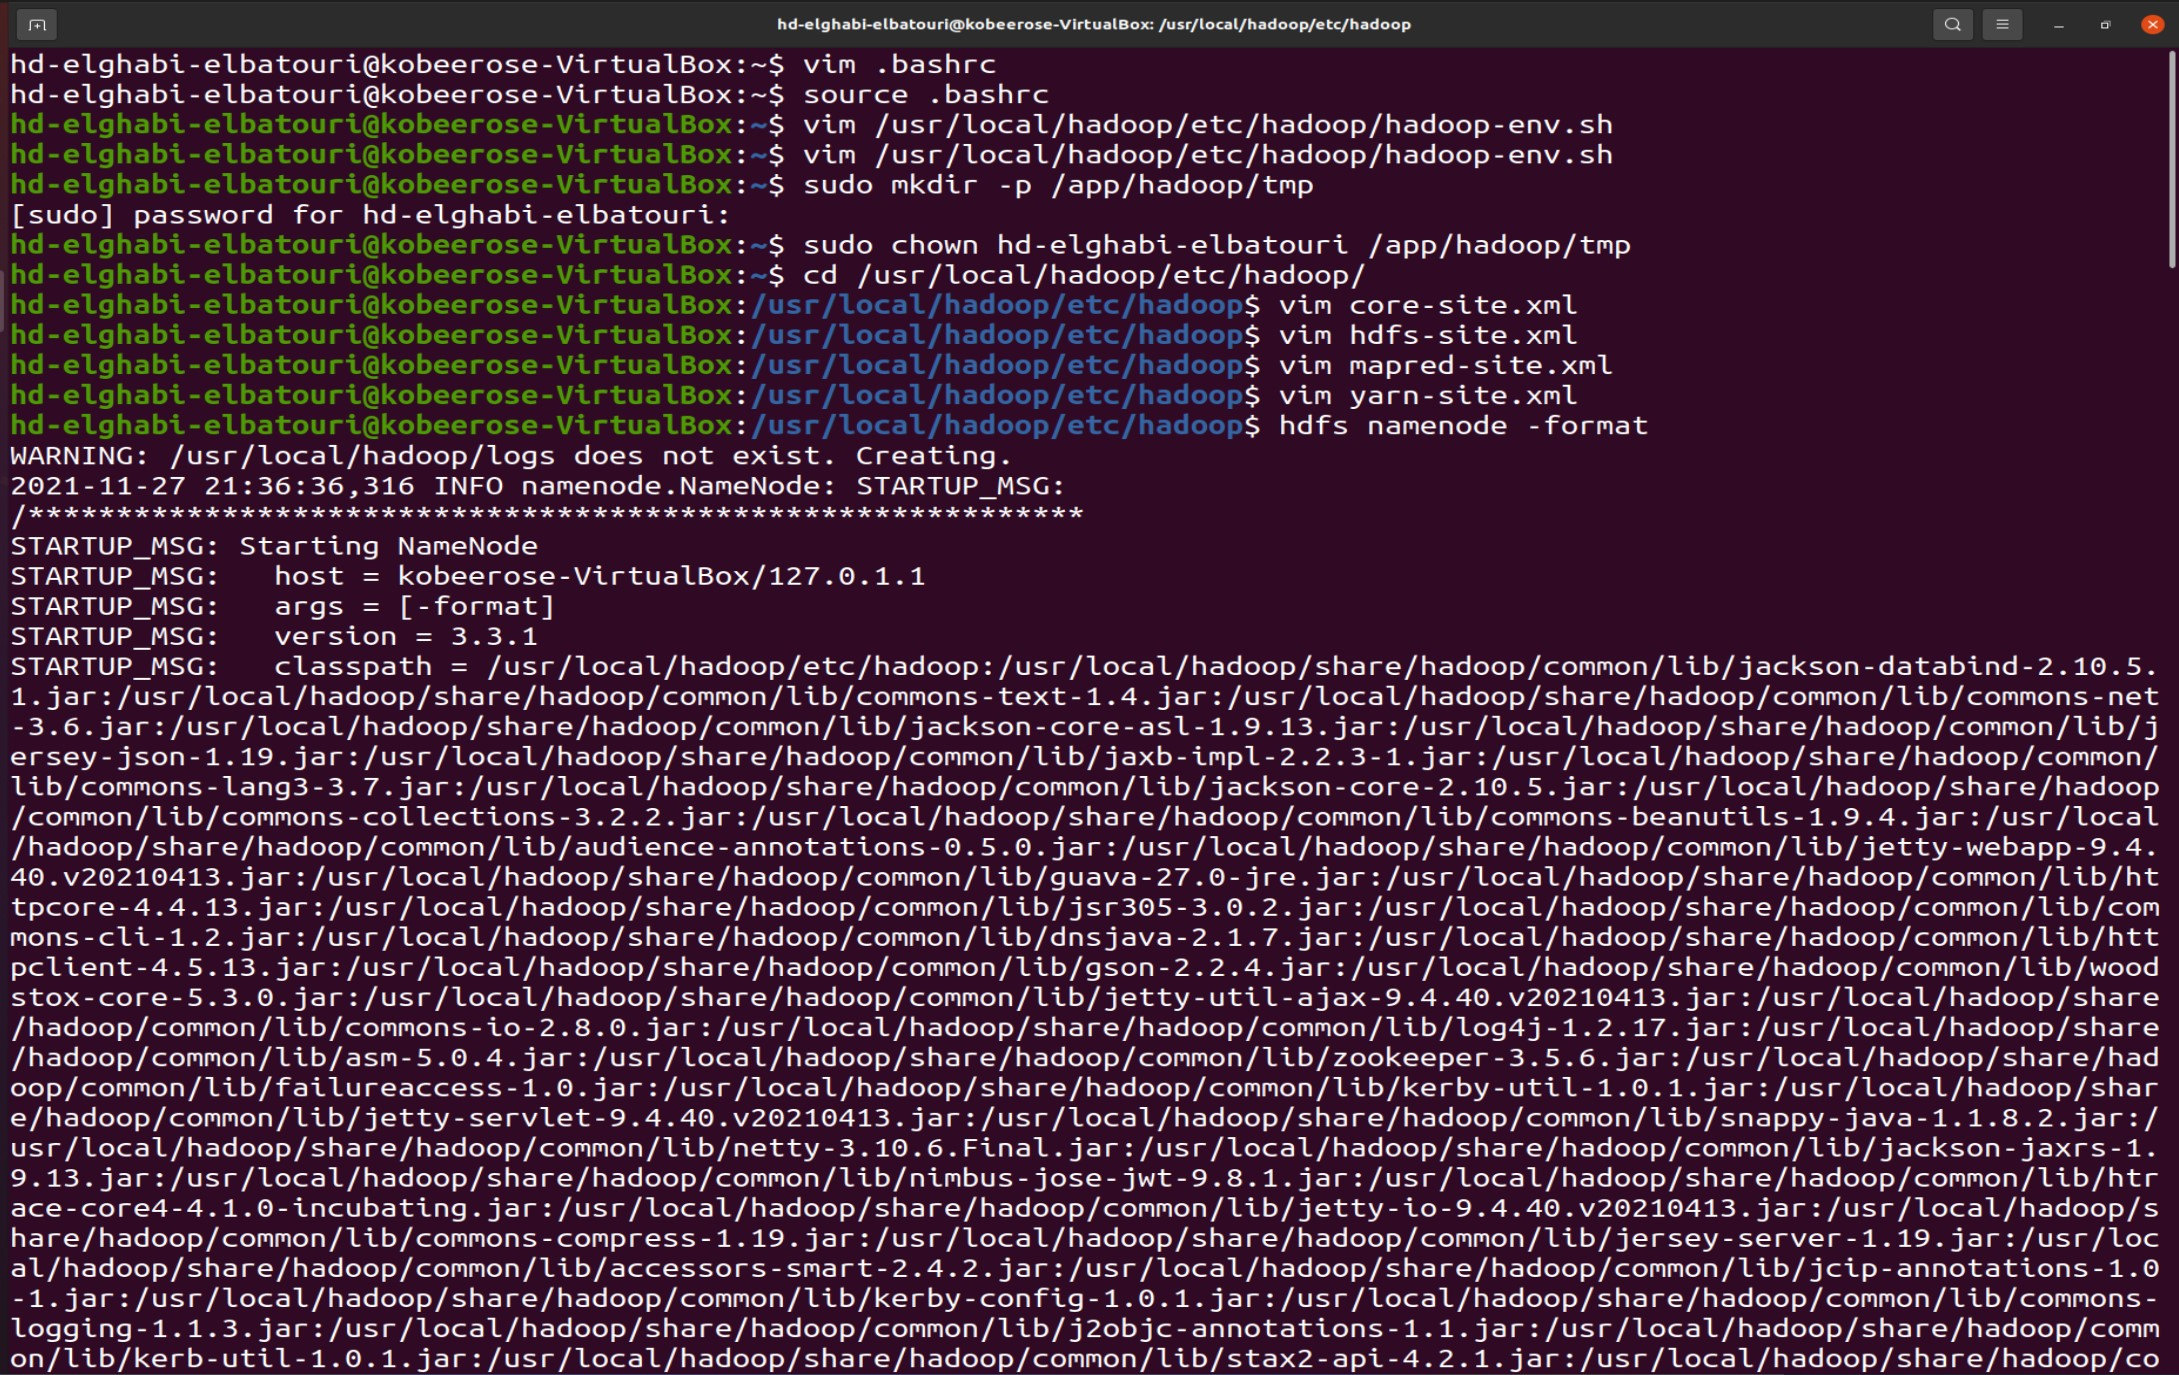
\includegraphics[width=1\linewidth]{Big_Data/Hadoop/Apache Hadoop Installation/Hadoop files configuration} 
\end{center} 
\caption{Hadoop files configuration} 
\end{figure} 
\FloatBarrier

\par Now it's time to start the newly installed single node cluster. 
\\
\begin{figure}[!htb] 
\begin{center} 
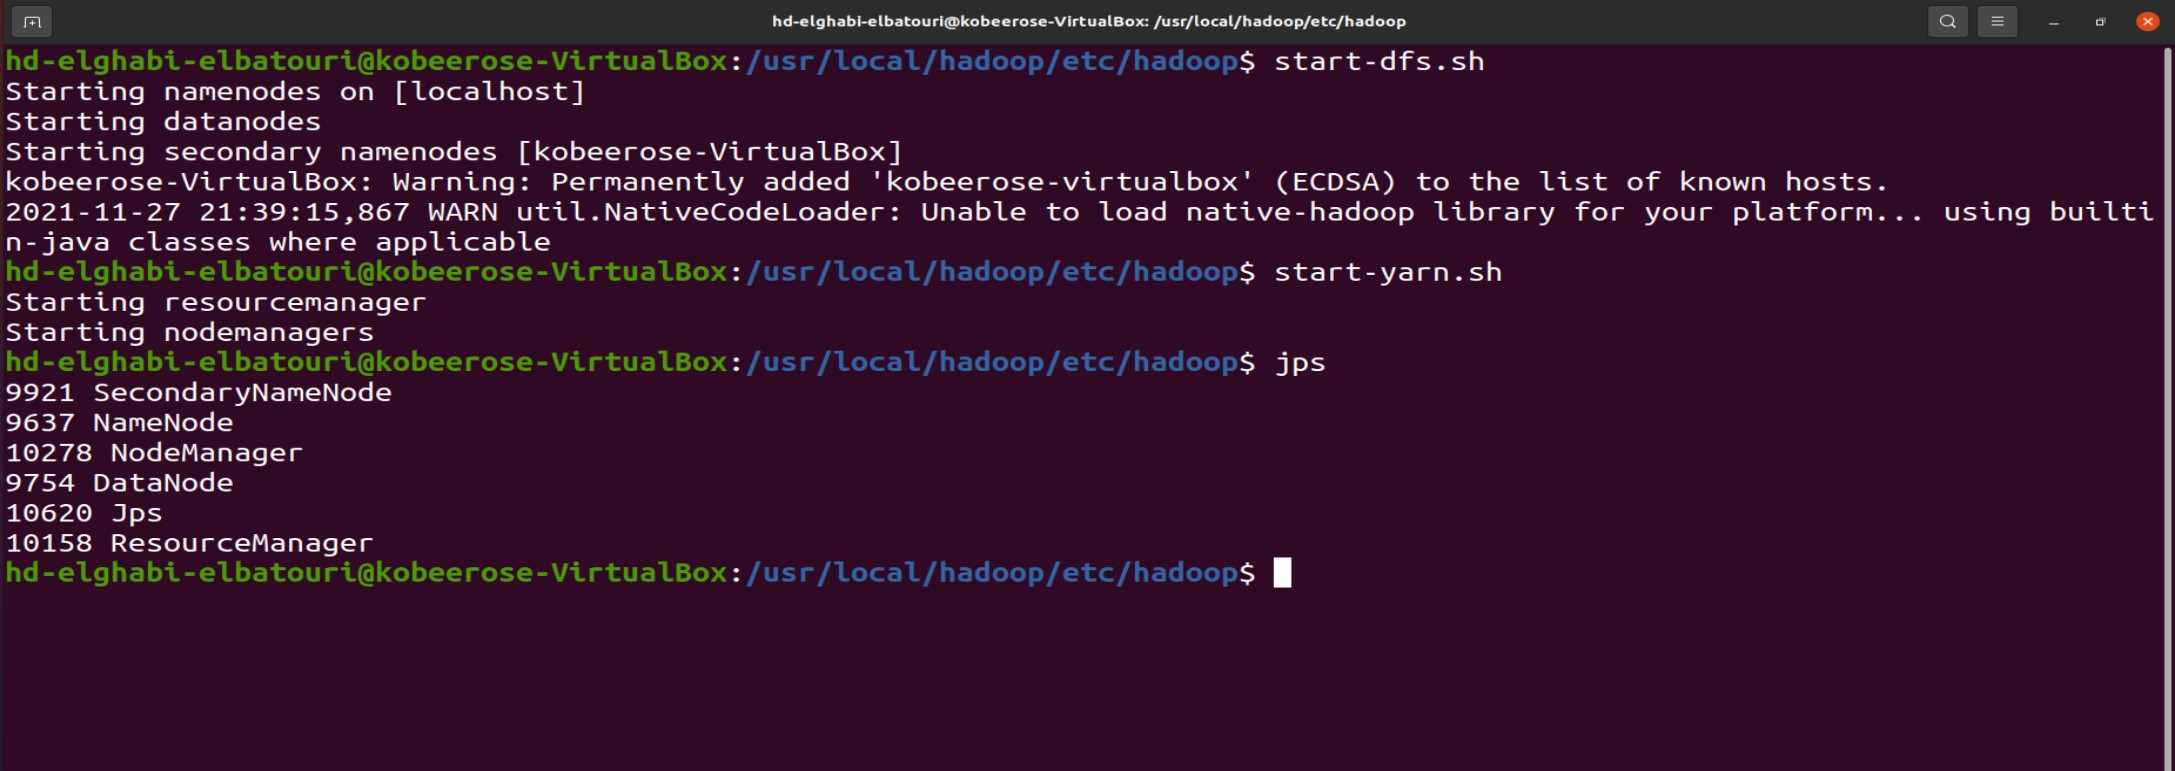
\includegraphics[width=1\linewidth]{Big_Data/Hadoop/Apache Hadoop Installation/Starting 1node Cluster} 
\end{center} 
\caption{Starting 1node Cluster} 
\end{figure} 
\FloatBarrier

\par Access Hadoop's graphical interfaces via the browser.
\\
\begin{figure}[!htb] 
\begin{center} 
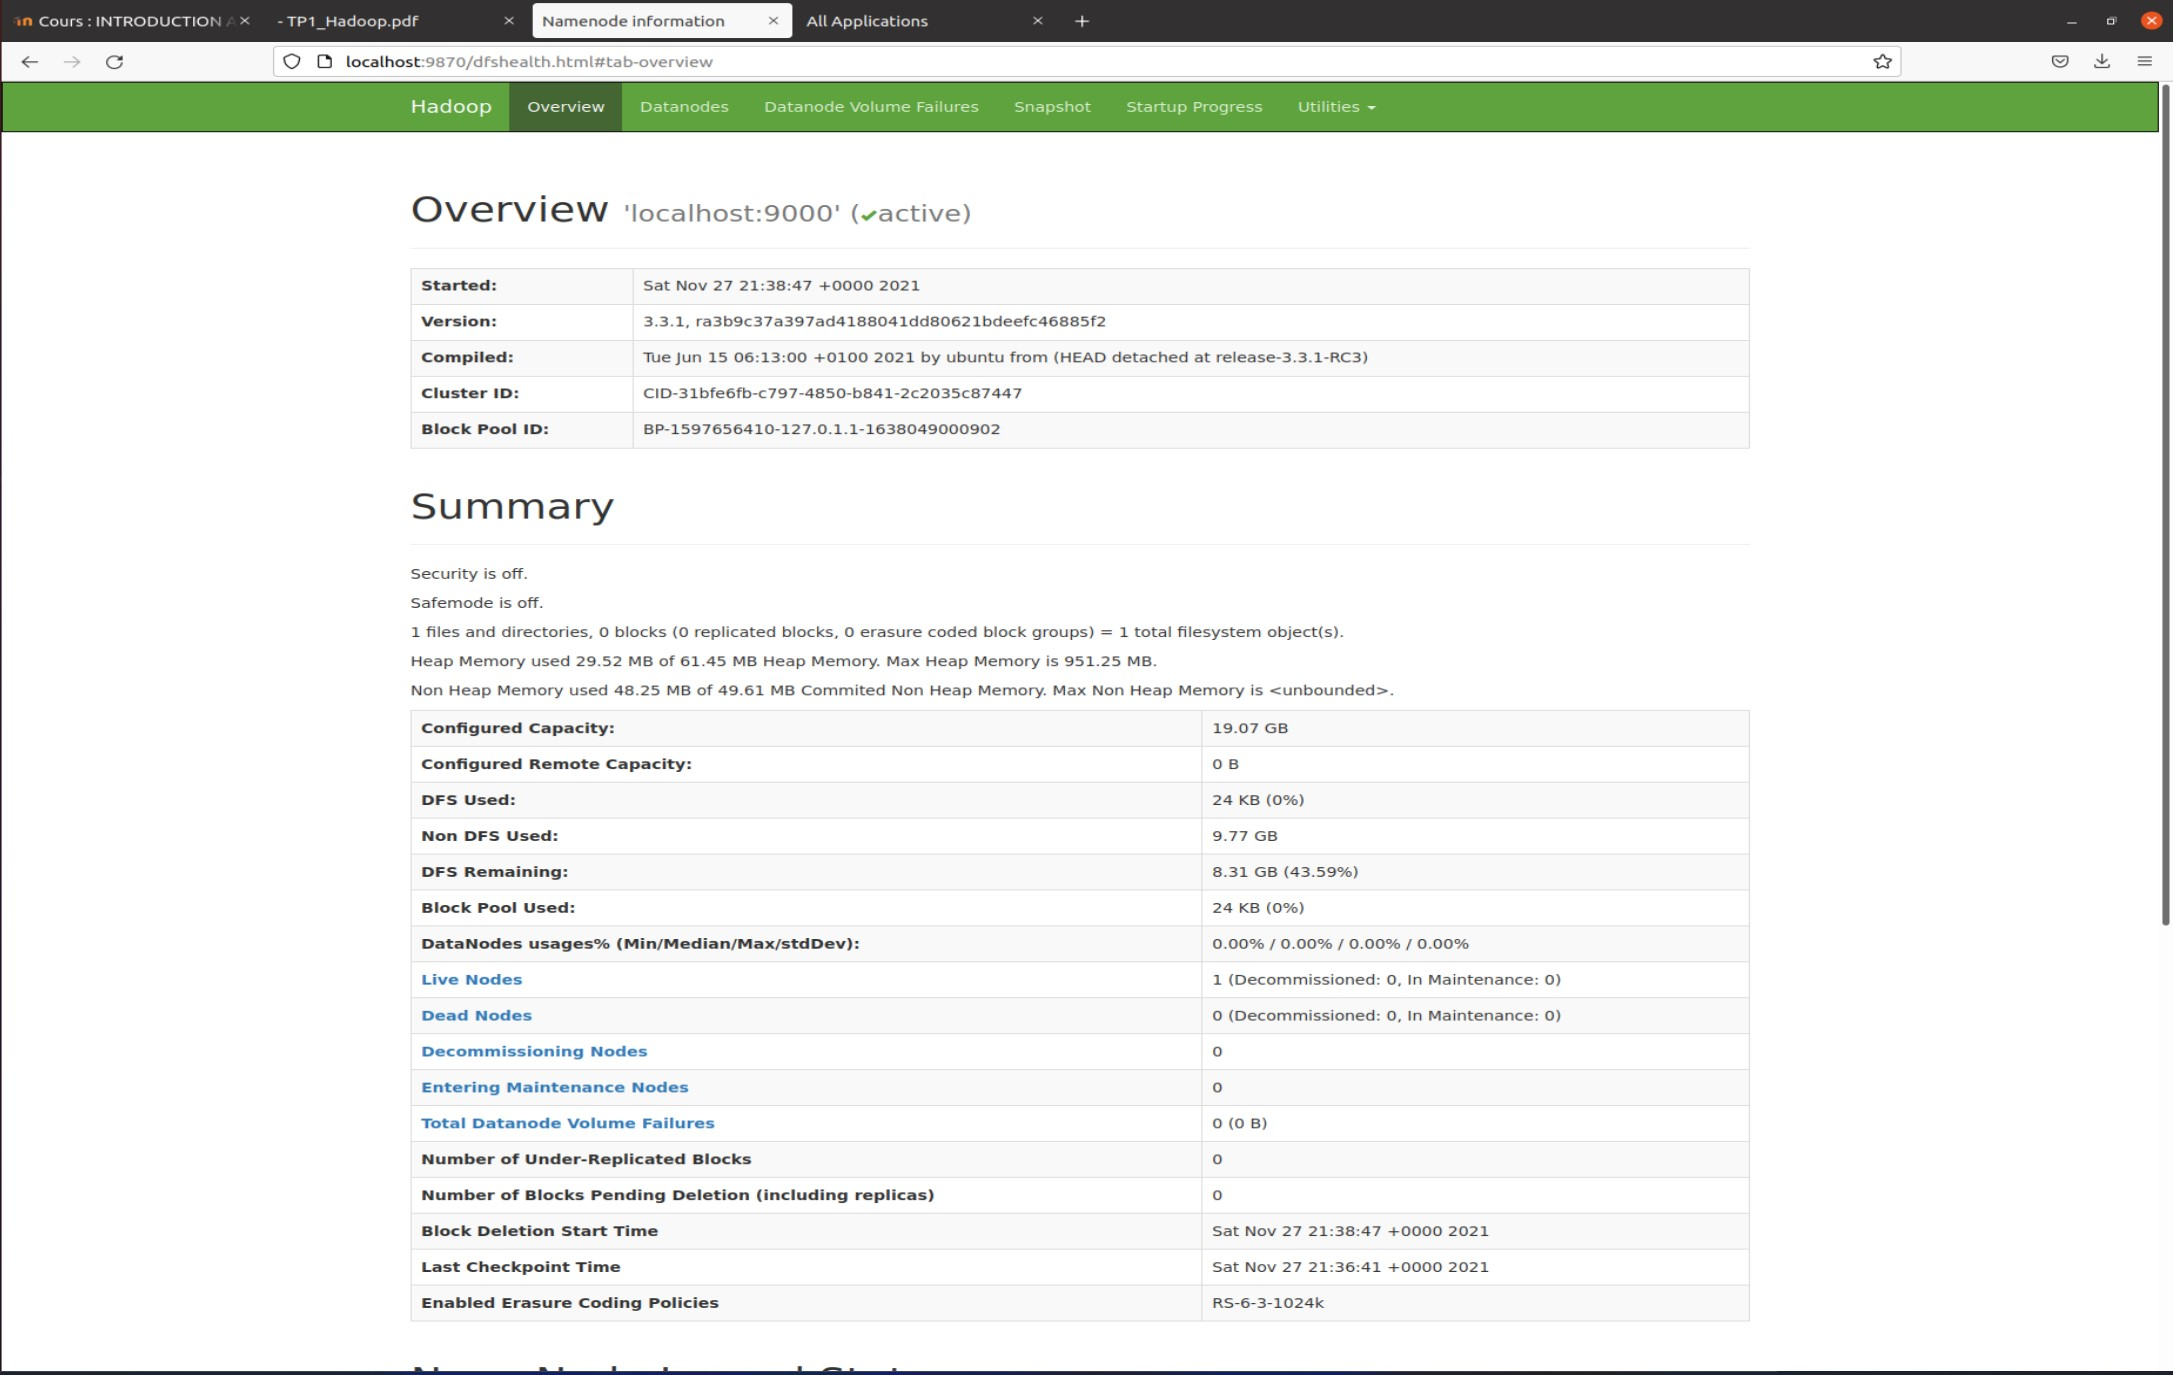
\includegraphics[width=1\linewidth]{Big_Data/Hadoop/Apache Hadoop Installation/Hadoop interface on port 9870} 
\end{center} 
\caption{Hadoop interface on port 9870} 
\end{figure} 
\FloatBarrier
\\
\begin{figure}[!htb] 
\begin{center} 
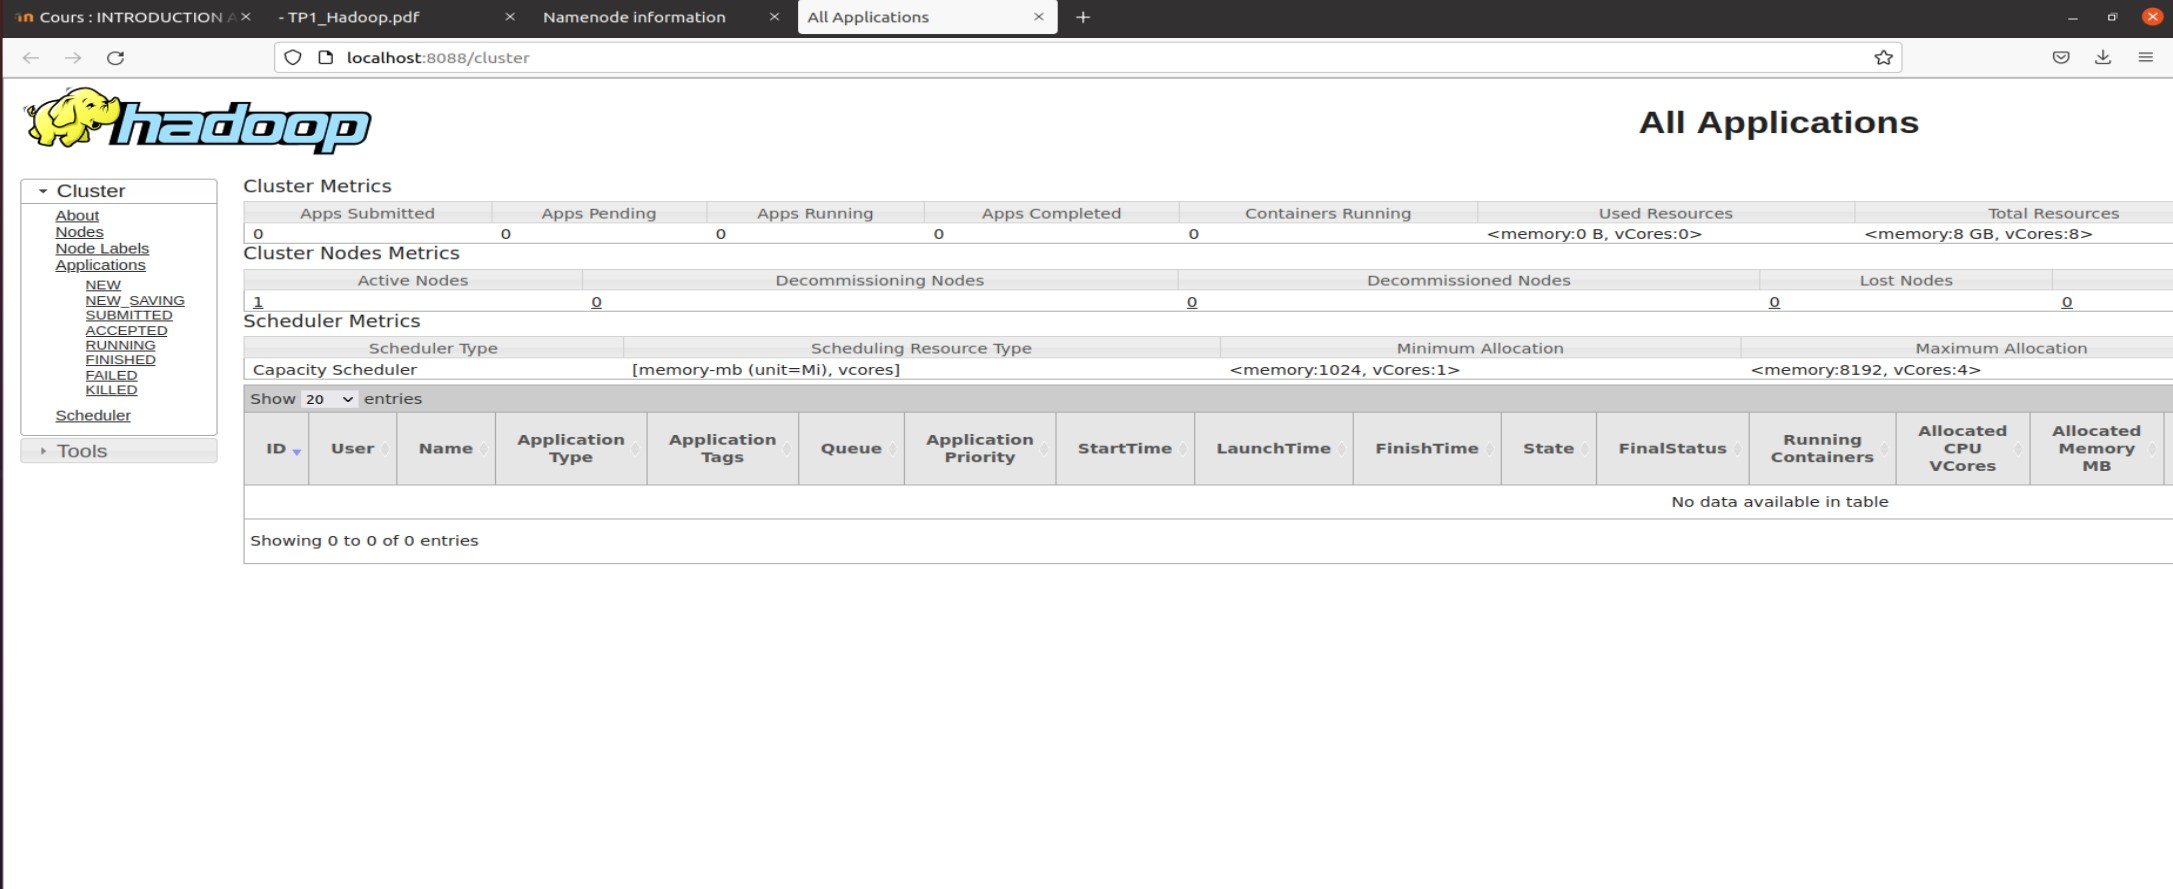
\includegraphics[width=1\linewidth]{Big_Data/Hadoop/Apache Hadoop Installation/ResourceManager Interface} 
\end{center} 
\caption{ResourceManager Interface} 
\end{figure} 
\FloatBarrier




\end{spacing}

\chapter{Pre-Requirementsuration Setup}
\par Now whit our envirement ready to use, we will be installing Openstack Victoria that will help us to build our private cloud, RabbitMQ as message streaming, broker and messaging queue implementation that Openstack services will use in order to communicate since we are in the context of a distributed system. And finally Memcached to ensure that our system will have a caching protocol that fit our distributed system; caching is used to keep important and most demanded information fast to access an store it in memory rather than the hard-drive.
\begin{spacing}{1.2}
%note en bas de page
\section{Openstack Victoria}

\par The installation of centos-release-openstack-victoria, rabbitmq-server and memcached is done via dnf. A
After installation is complete, an update of the CentOS System is required. 
\\
\begin{figure}[!htb] 
\begin{center} 
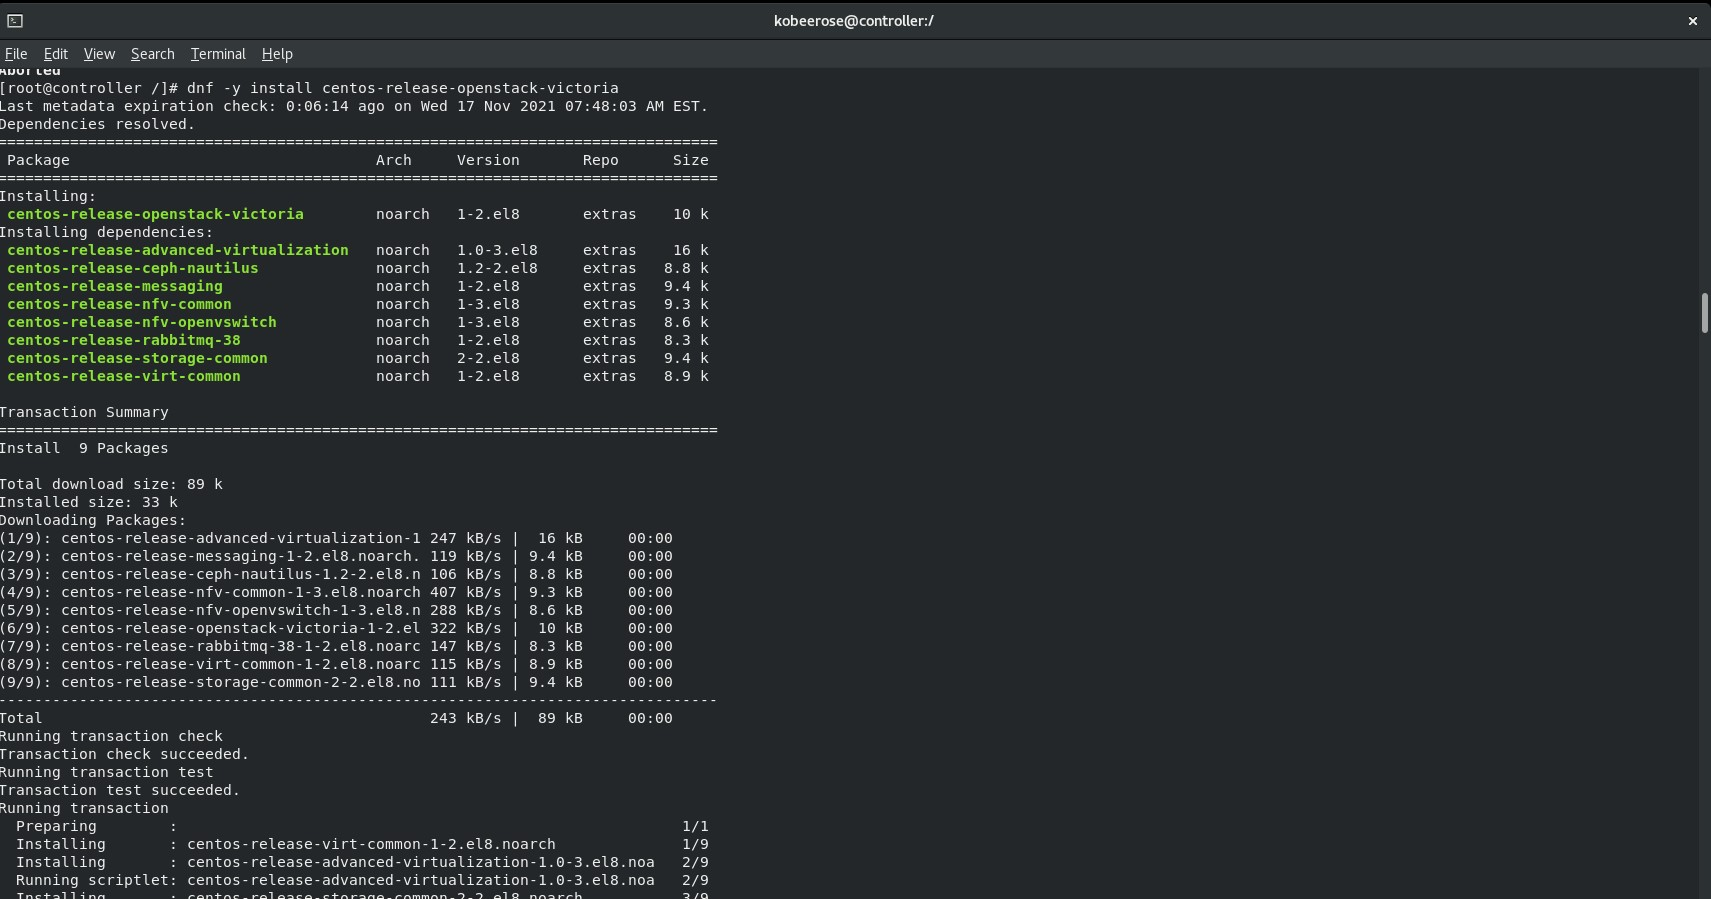
\includegraphics[width=1\linewidth]{Cloud/Pre-Requirements/Installing openstack-victoria} 
\end{center} 
\caption{Installing openstack-victoria} 
\end{figure}  \FloatBarrier
\\
\\
\begin{figure}[!htb] 
\begin{center} 
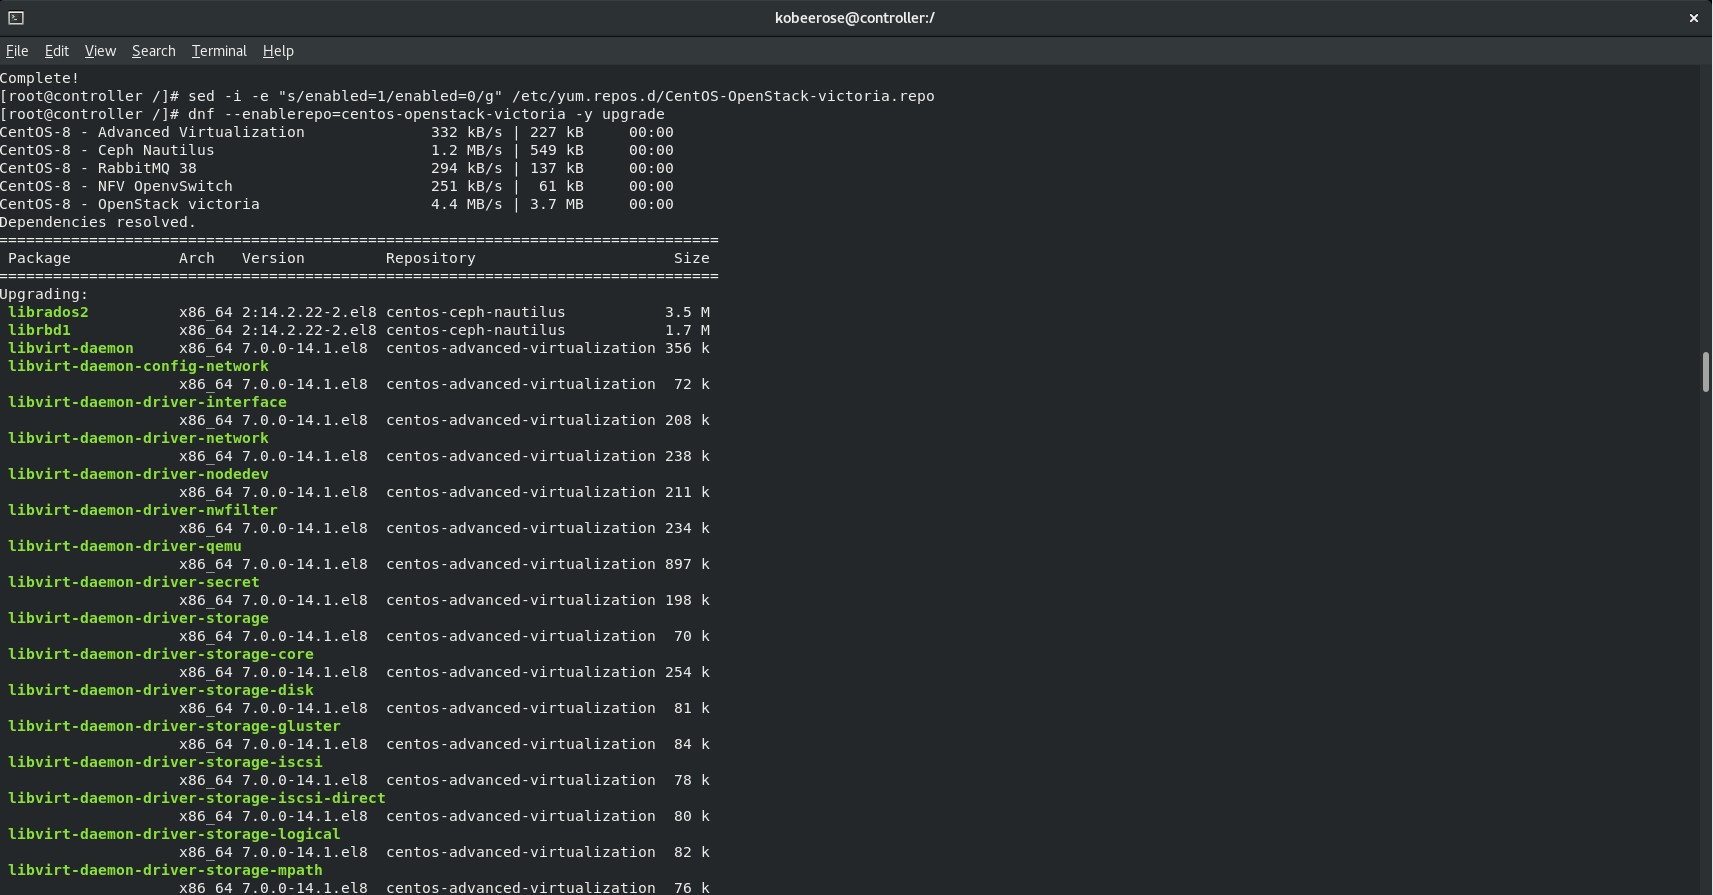
\includegraphics[width=1\linewidth]{Cloud/Pre-Requirements/Add Openstack Repo _ Upgrade CentOS System} 
\end{center} 
\caption{Add Openstack Repo _ Upgrade CentOS System} 
\end{figure}  \FloatBarrier
\\

\section{Installation of RabbitMQ, Memcached.}

\par First of all we need to install RabbitMQ server
\\
\begin{figure}[!htb] 
\begin{center} 
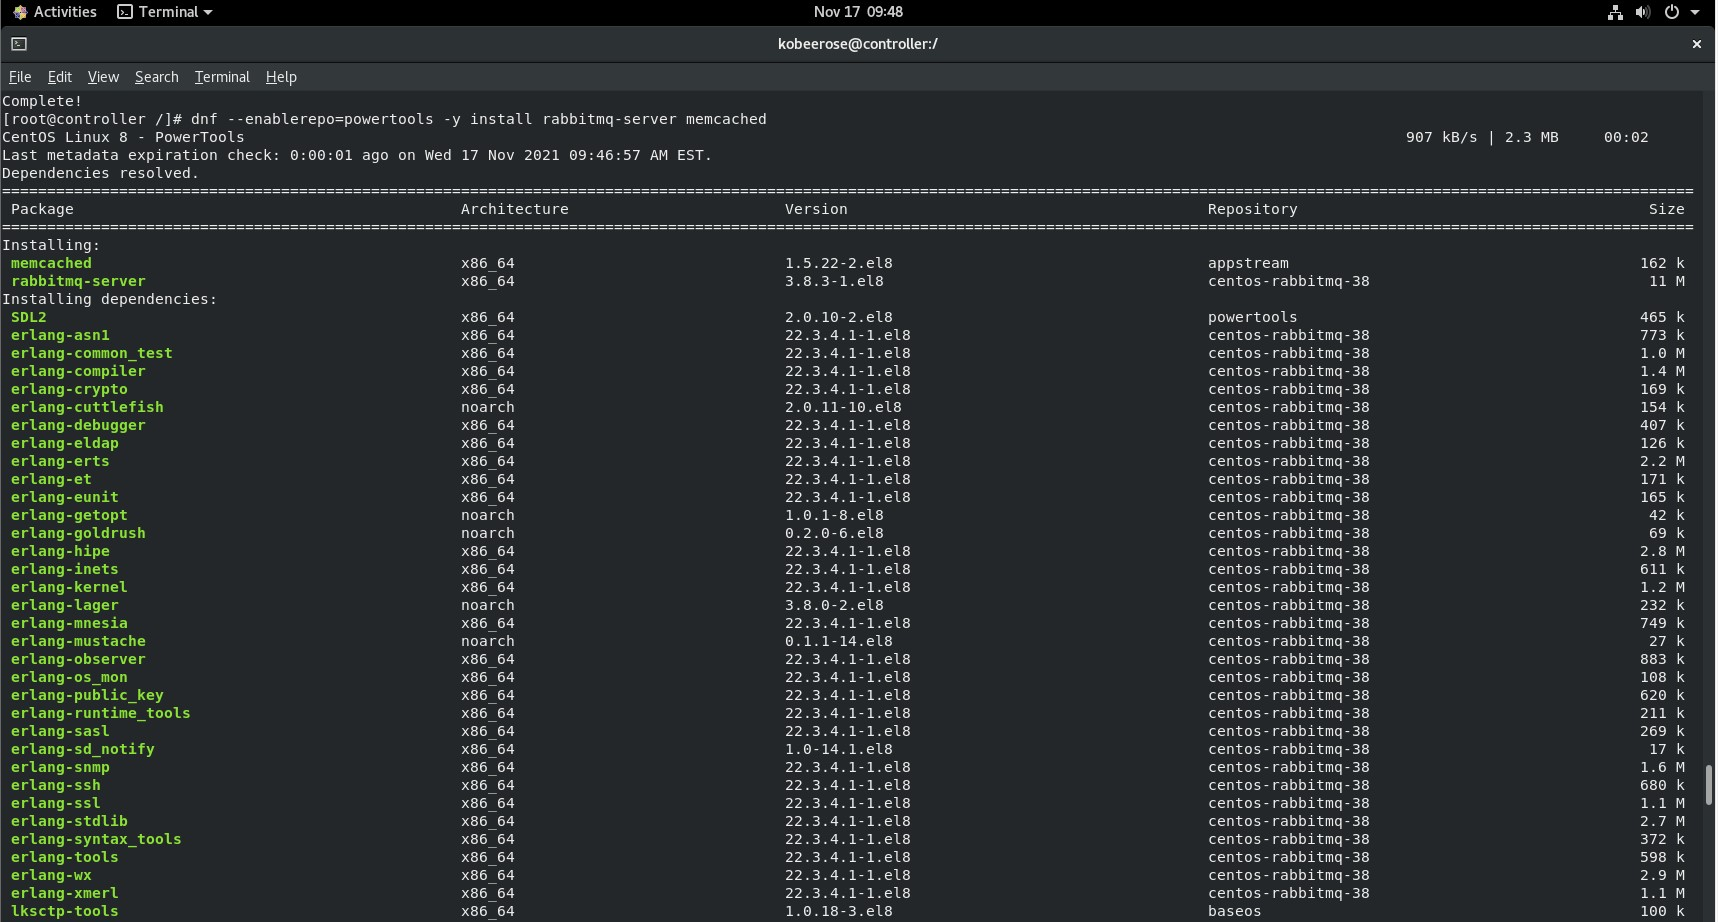
\includegraphics[width=1\linewidth]{Cloud/Pre-Requirements/Installing rabbitmq-server} 
\end{center} 
\caption{Installing rabbitmq-server} 
\end{figure}  \FloatBarrier
\\
\par We are going to change in the file /etc/my.cnf.d/mariadb-server.cnf the default value 151
which is not sufficient in the Openstack environment. And to consider the modifications, we
let's restart and enable mariadb rabbitmq-server and memcached. 
\\
\begin{figure}[!htb] 
\begin{center} 
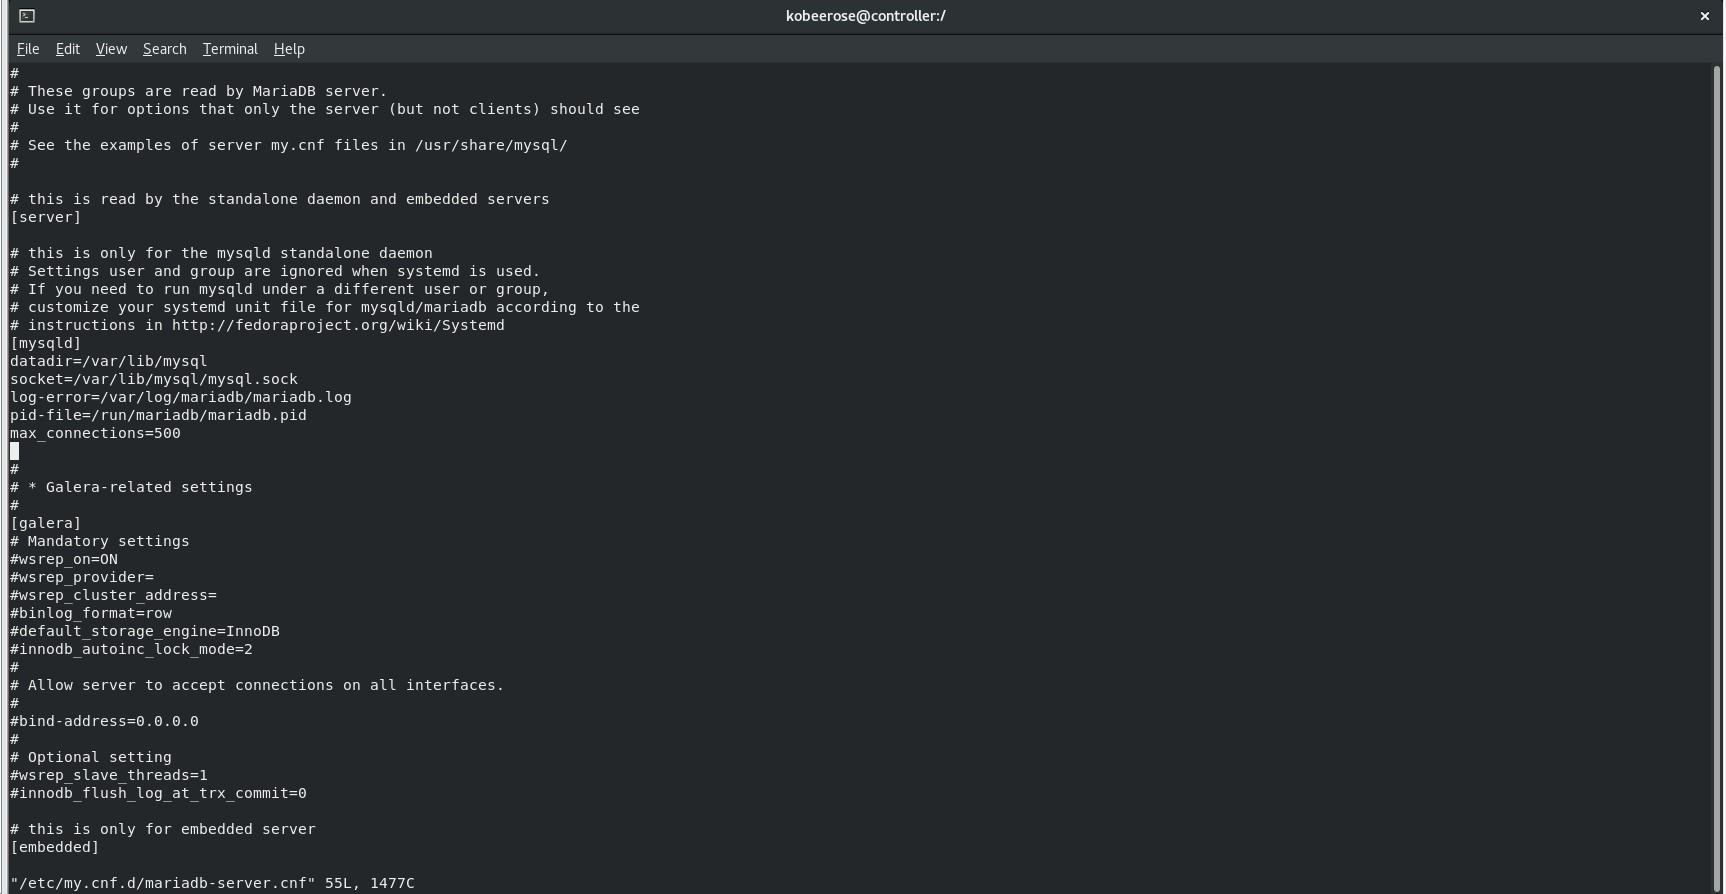
\includegraphics[width=1\linewidth]{Cloud/Pre-Requirements/changing max_connections} 
\end{center} 
\caption{changing max connections} 
\end{figure}  \FloatBarrier
\\
\par now we persue with configuring the memcached file in order to listen to all
\\
\begin{figure}[!htb] 
\begin{center} 
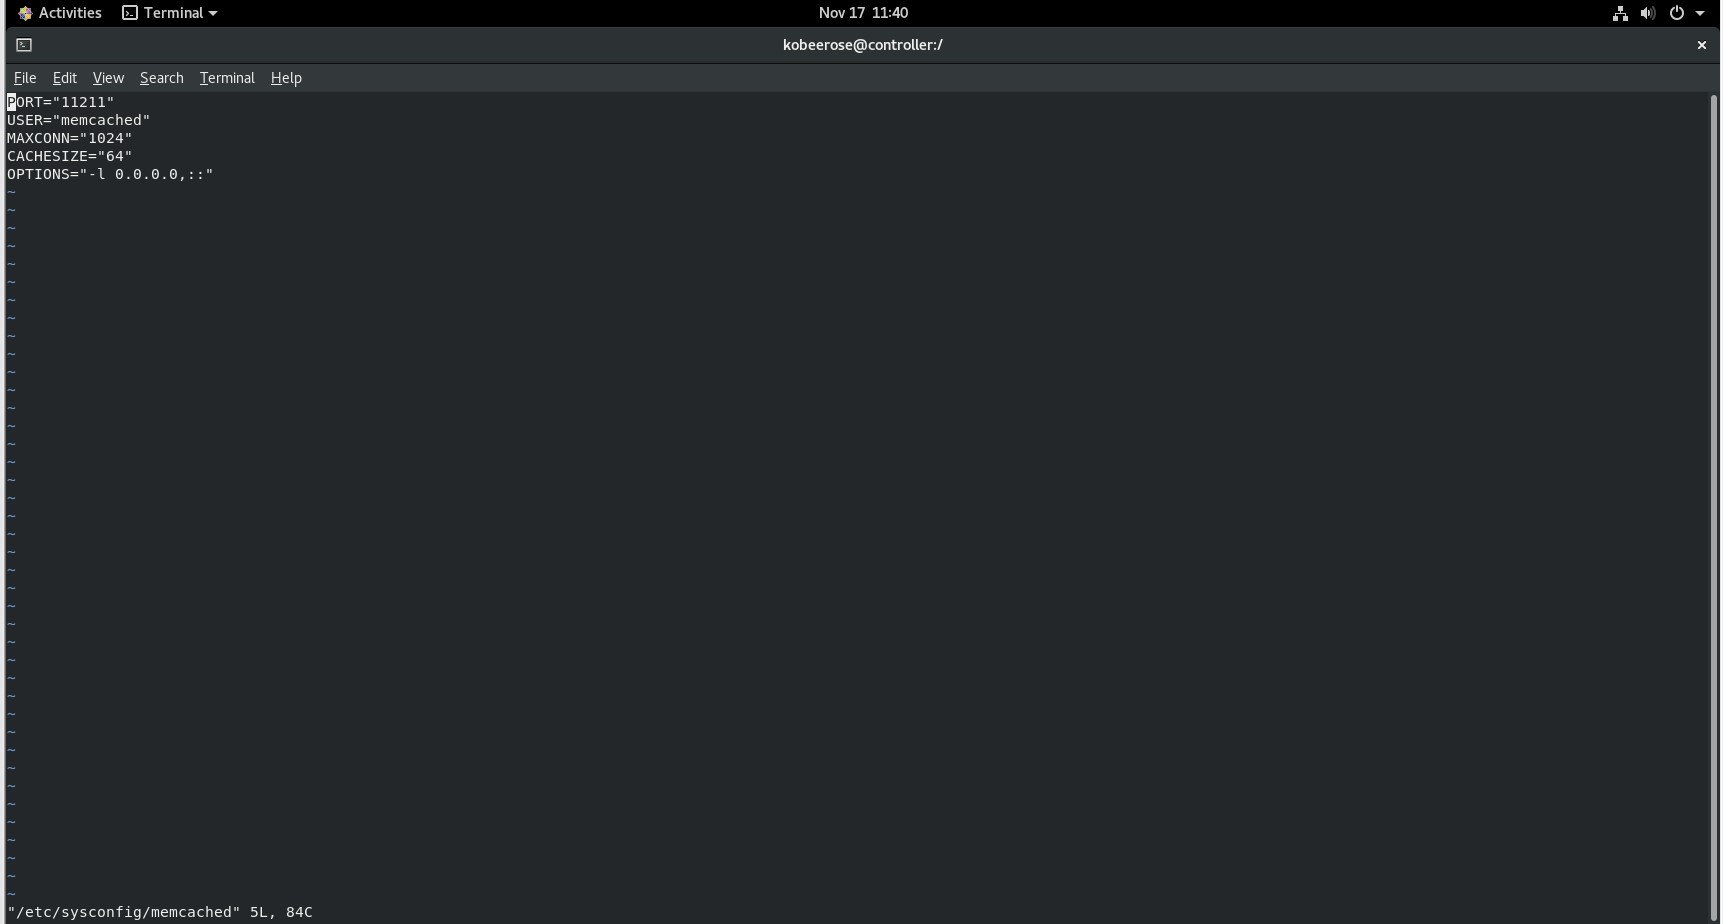
\includegraphics[width=1\linewidth]{Cloud/Pre-Requirements/memcached config} 
\end{center} 
\caption{memcached config} 
\end{figure}  \FloatBarrier
\\
\section{rabbitmqctl config }
\\
\par After that, we will add a new openstack user, define a password for him.
, also give it all the permissions and if SELinux is enabled, we have to change the policy
via a rabbitmqctl.te file and We will use the checkmodule and semodule commands to verify and compile this module.
of SELinux security policy in a binary representation8 
\\
\begin{figure}[!htb] 
\begin{center} 
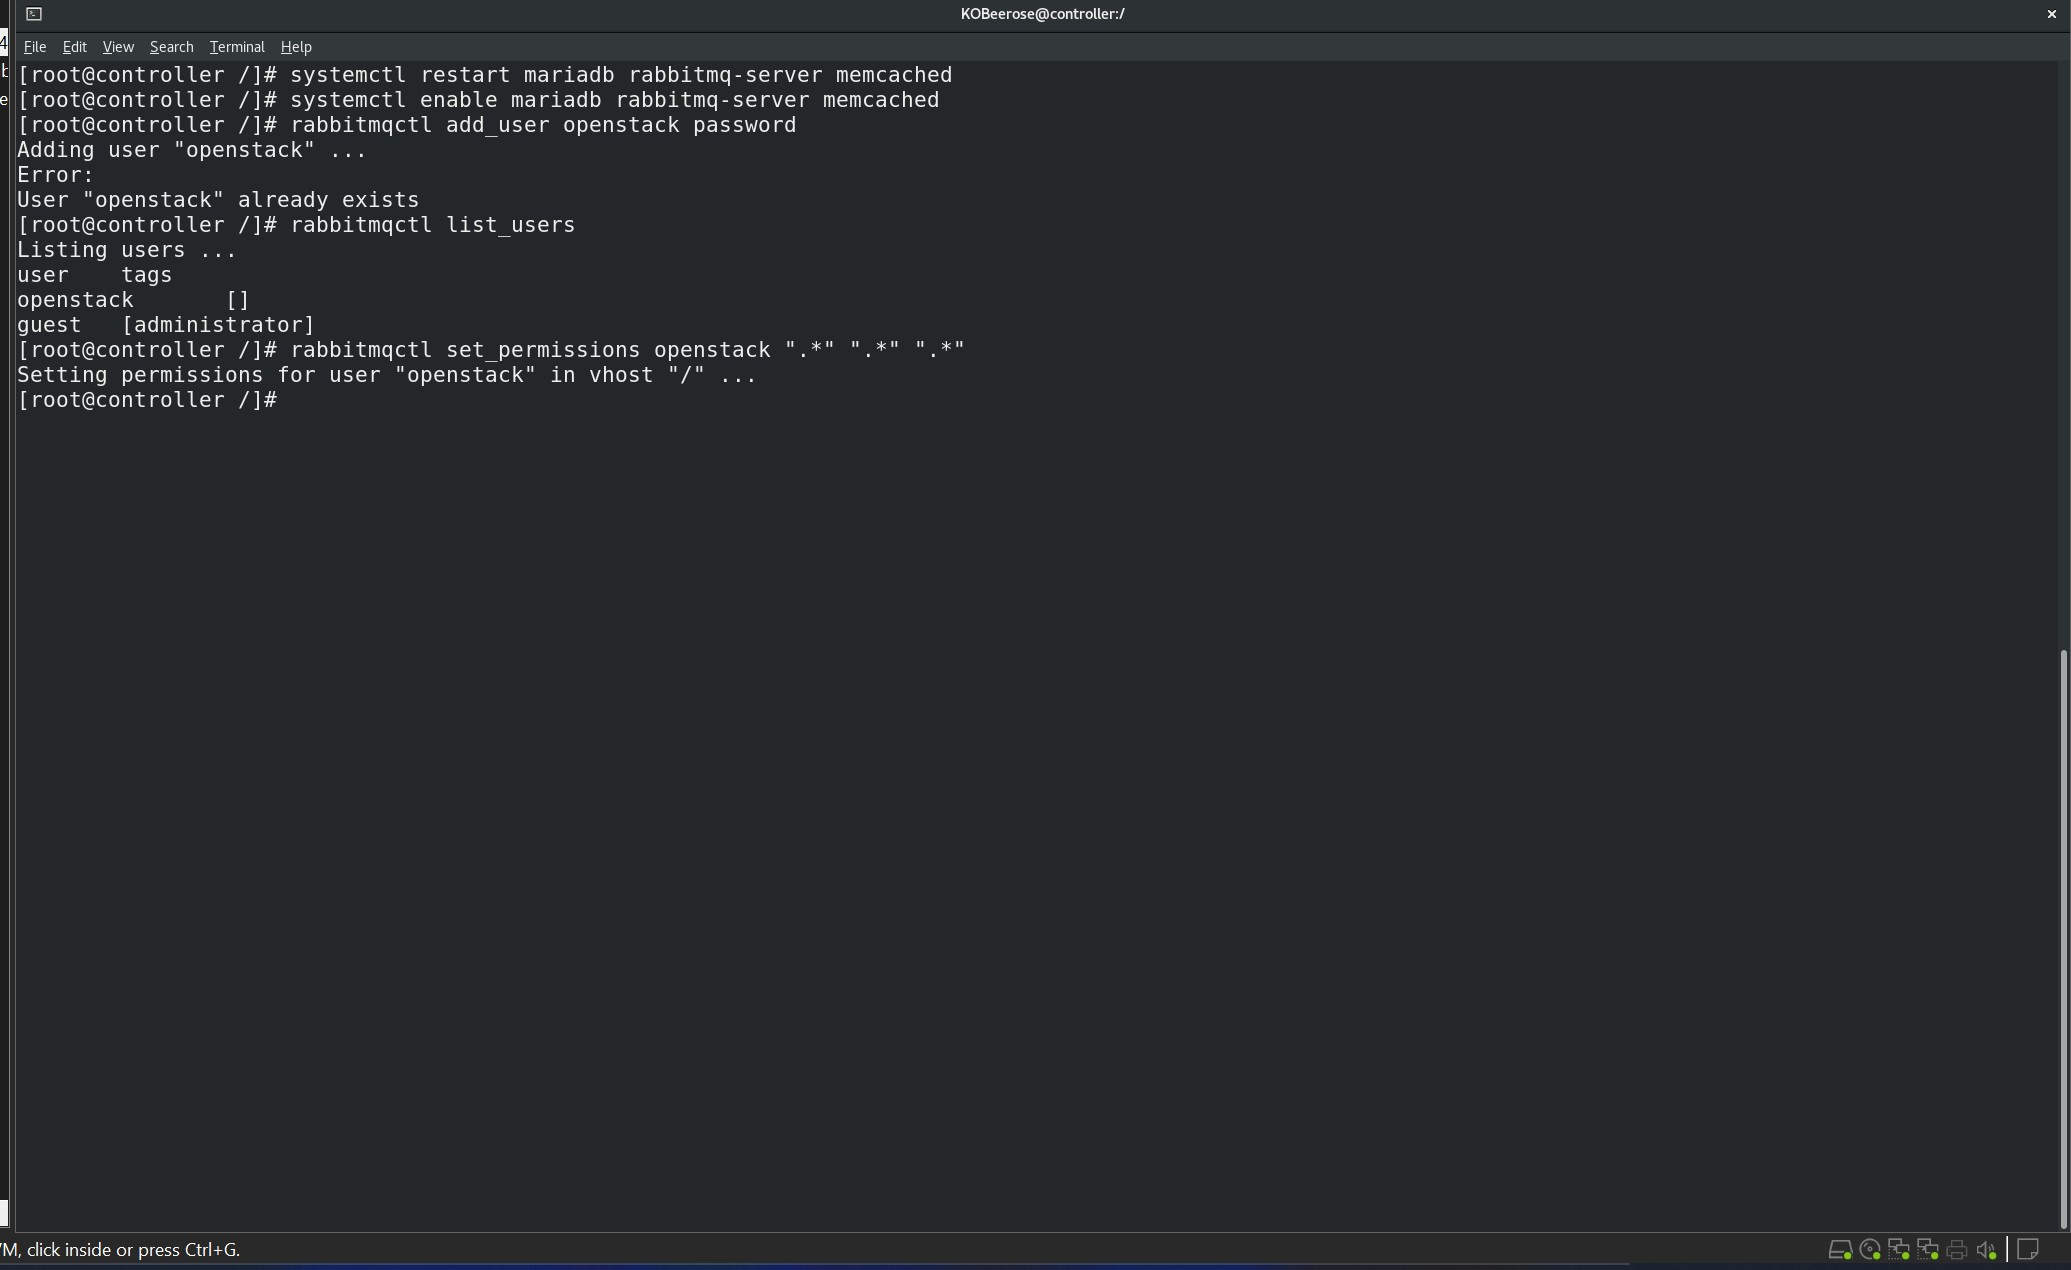
\includegraphics[width=1\linewidth]{Cloud/Pre-Requirements/Creating a new openstack user} 
\end{center} 
\caption{Creating a new openstack user} 
\end{figure}  \FloatBarrier
\\


\par Allowing mysql service, the port 5672 service and reloading the firewall.\\
\\
\begin{figure}[!htb] 
\begin{center} 
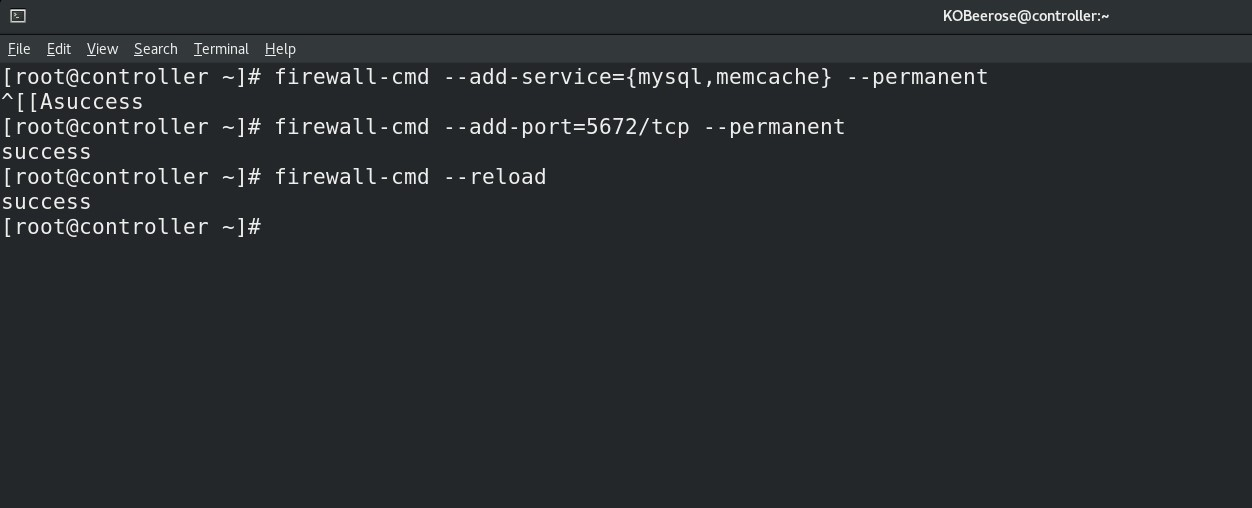
\includegraphics[width=.8\linewidth]{Cloud/Pre-Requirements/Allowing ports for services.} 
\end{center} 
\caption{Allowing ports for services.} 
\end{figure}  \FloatBarrier
\\


\end{spacing}
 
\chapter{Keystone Configuration}
\par based on the documentation, Keystone is an OpenStack service that provides API client authentication, service discovery, and distributed multi-tenant authorization by implementing OpenStack’s Identity API; which mean that keystone is the service that will be used as the authentication service and also will provide each user the services that he can use. And this section is dedicated to Keystone installation and configuration.
\begin{spacing}{1.2}
%note en bas de page
\section{Add a User and Database on MariaDB for Keystone}

\par In this section, we will install and configure OpenStack Identity Service (Keystone). We
are going to connect to MariaDb so that we can add a user and a database
for Keystone. 
\\
\begin{figure}[!htb] 
\begin{center} 
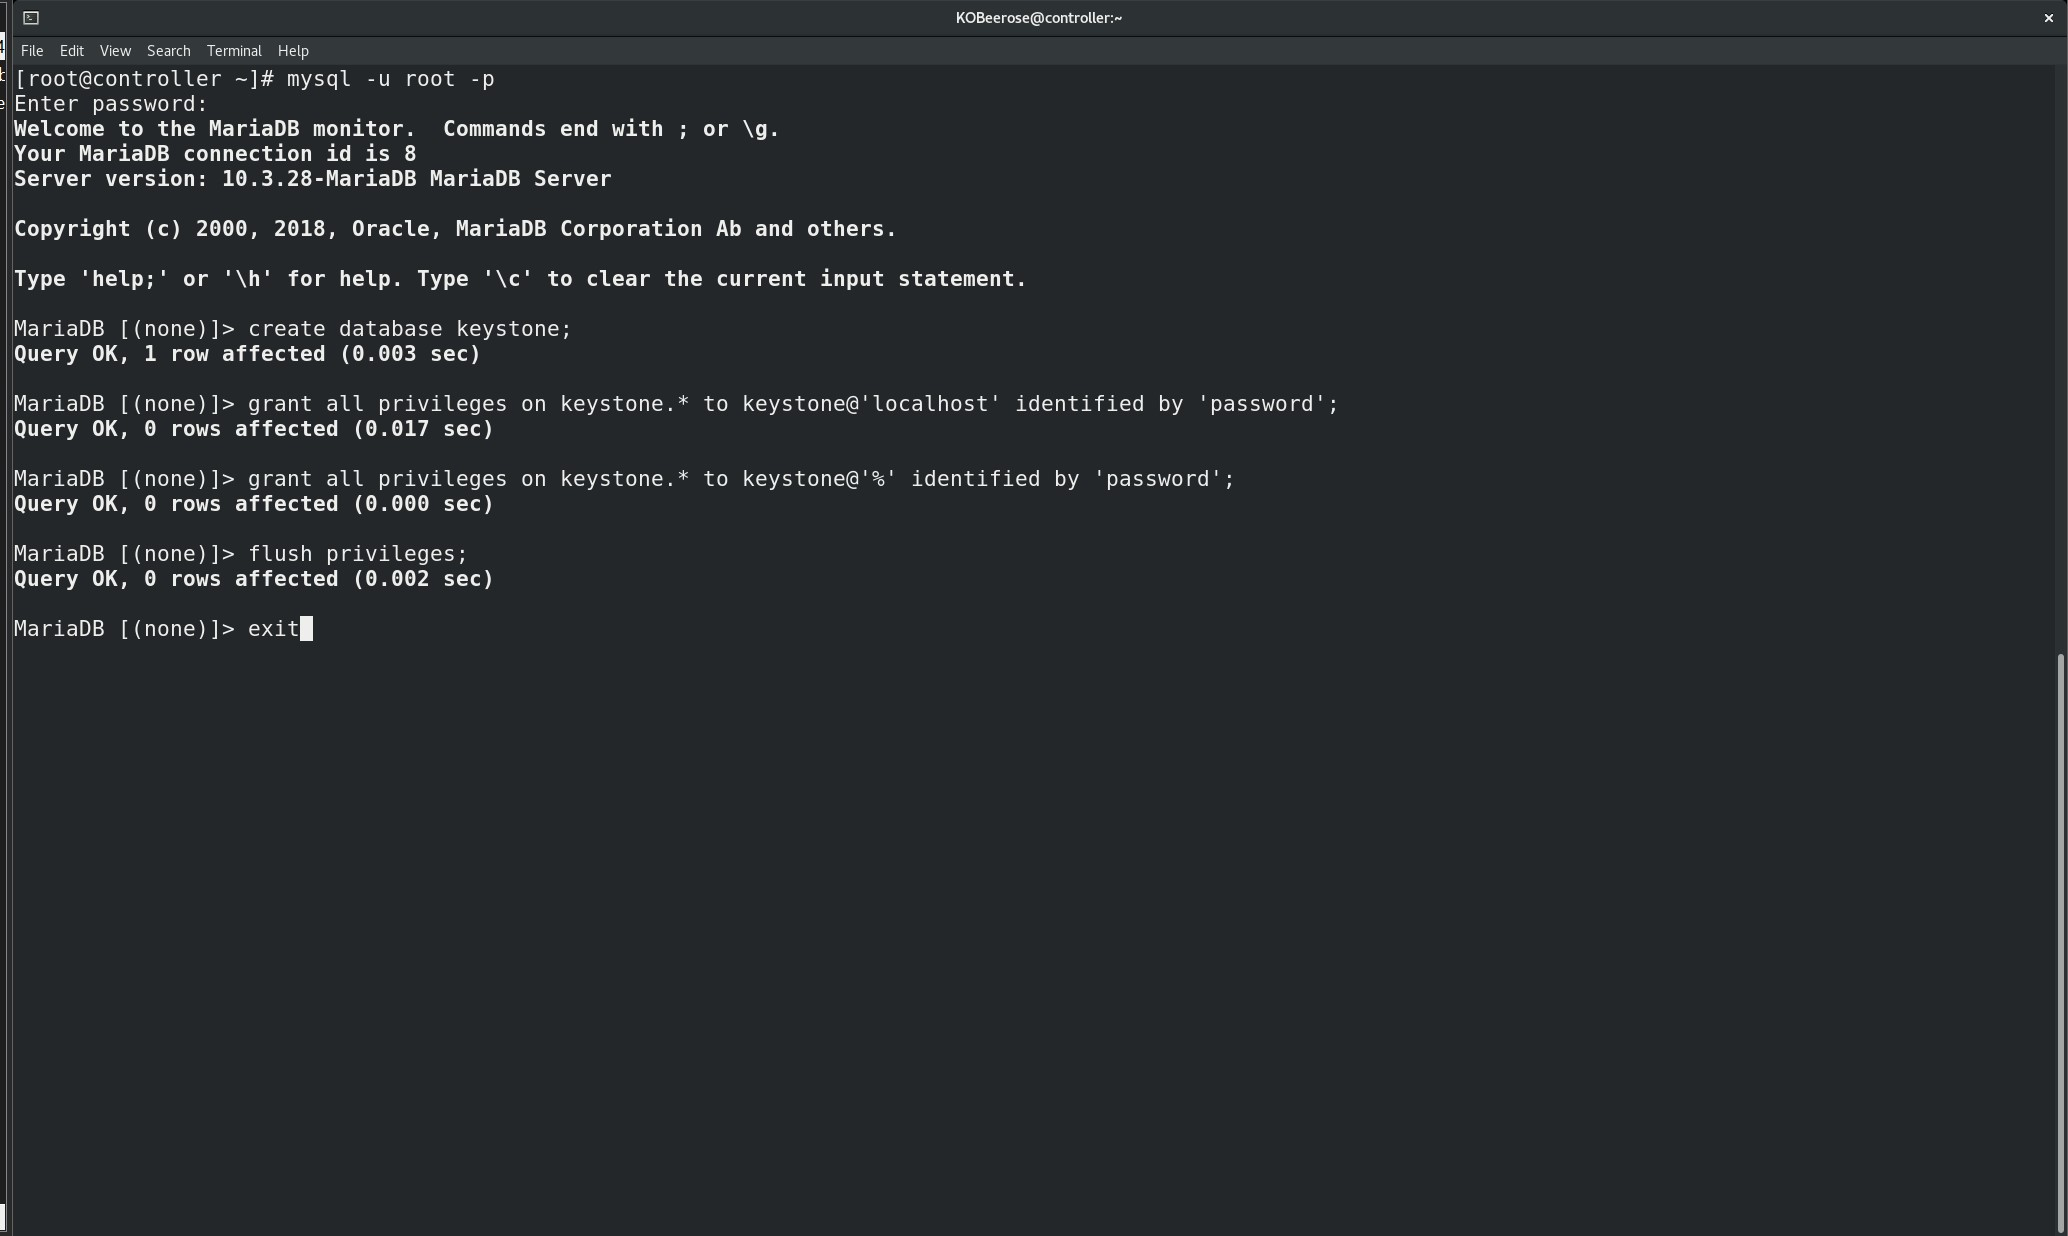
\includegraphics[width=1\linewidth]{Cloud/Configure Keystone #1/Add a user and DB for Keystone} 
\end{center} 
\caption{Add a user and DB for Keystone} 
\end{figure}  \FloatBarrier
\\


\section{Installing Keystone}

\par To install Keystone, we need to install many packages as shown in the
figure below: 
\\
\begin{figure}[!htb] 
\begin{center} 
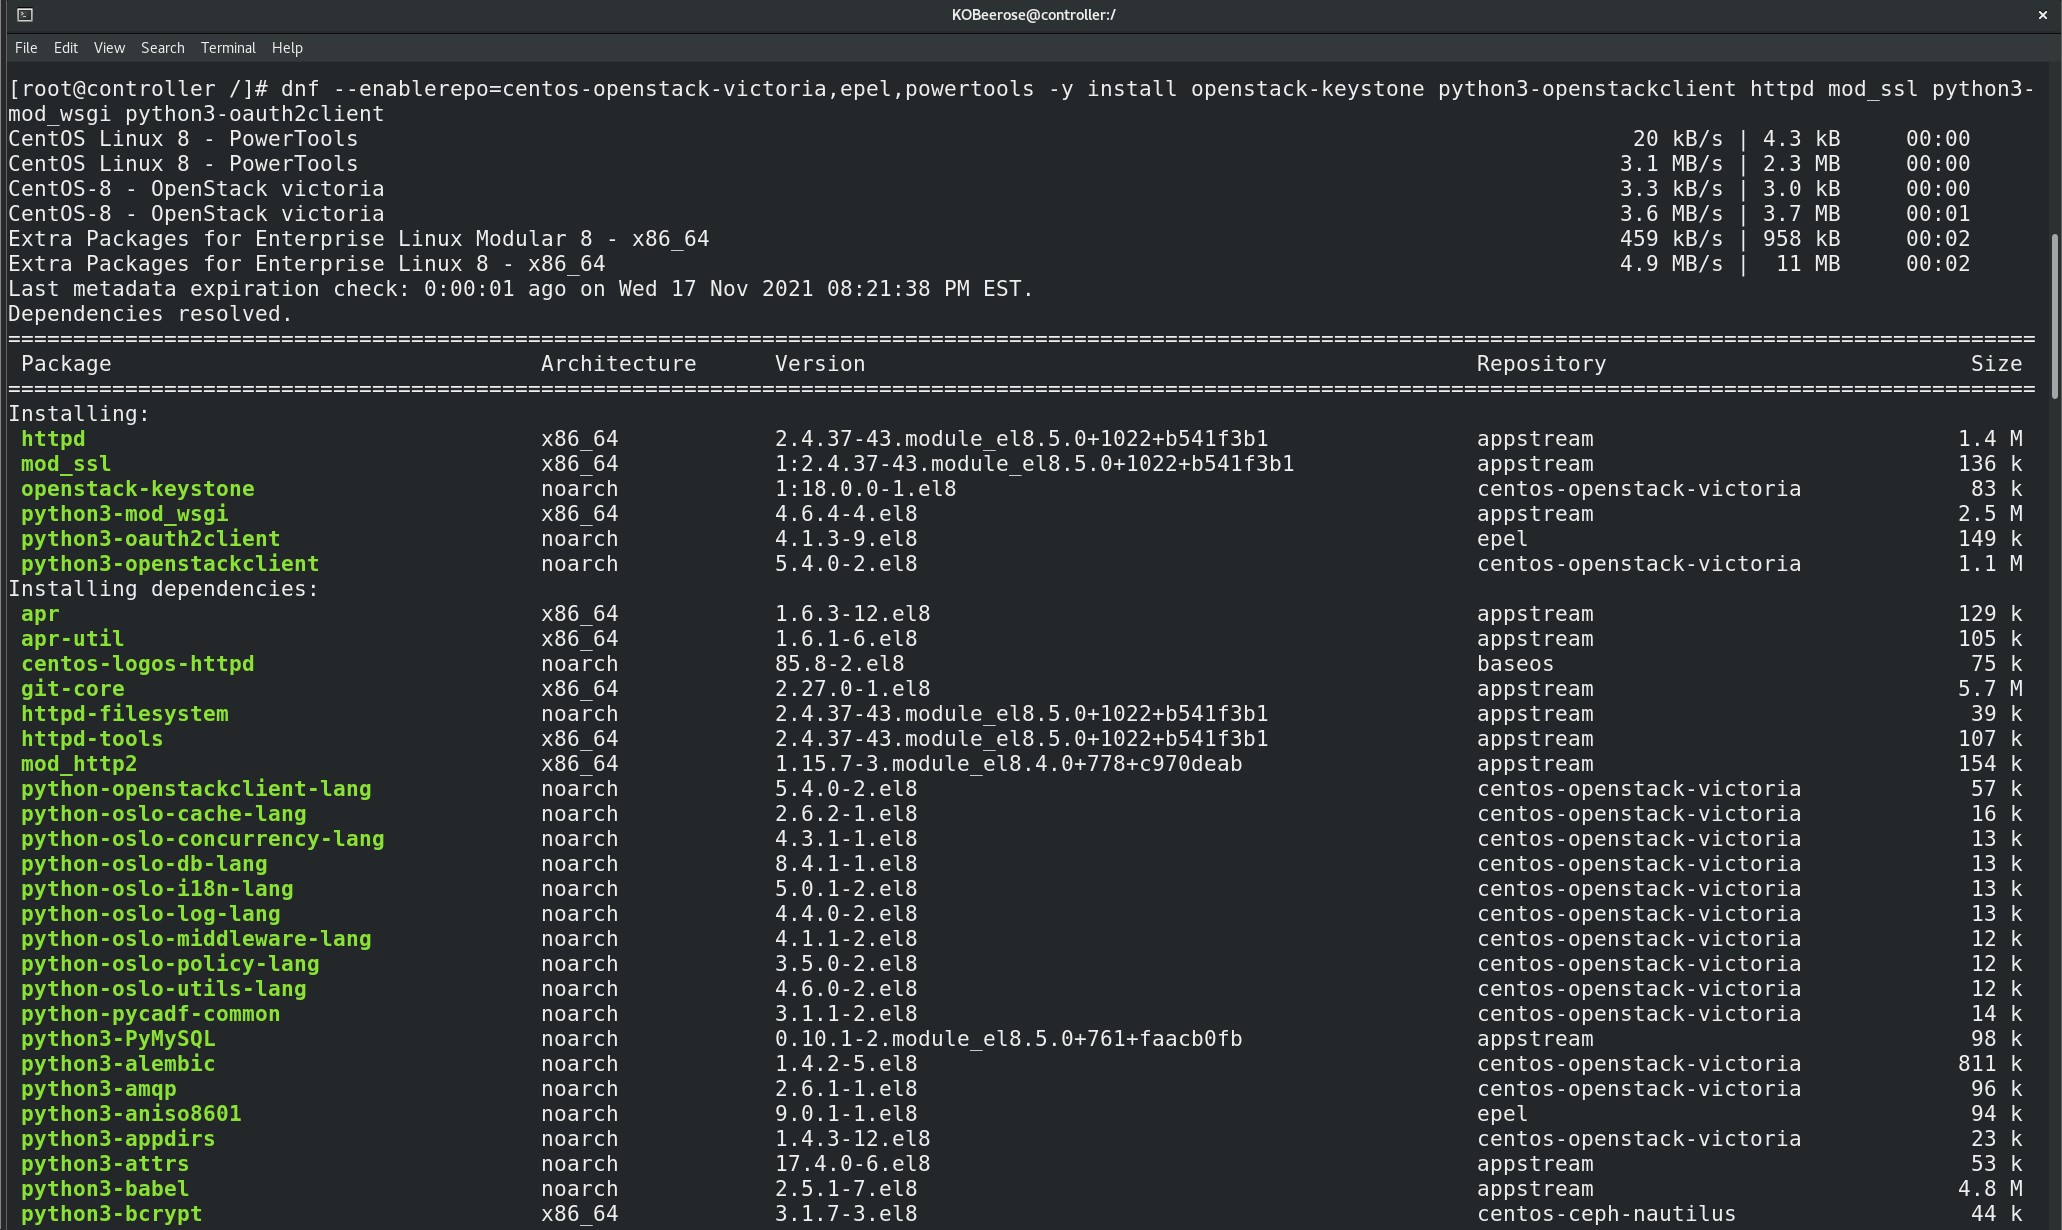
\includegraphics[width=1\linewidth]{Cloud/Configure Keystone #1/Installing EPEL, powertools} 
\end{center} 
\caption{Installing EPEL, powertools} 
\end{figure}  \FloatBarrier
\\


\section{Configure Keystone.}

\par To configure Keystone, we will specify the Memcache server, specify the information
MariaDB connection and comment on the Provider Fernet .\\

\\
\begin{figure}[!htb] 
\begin{center} 
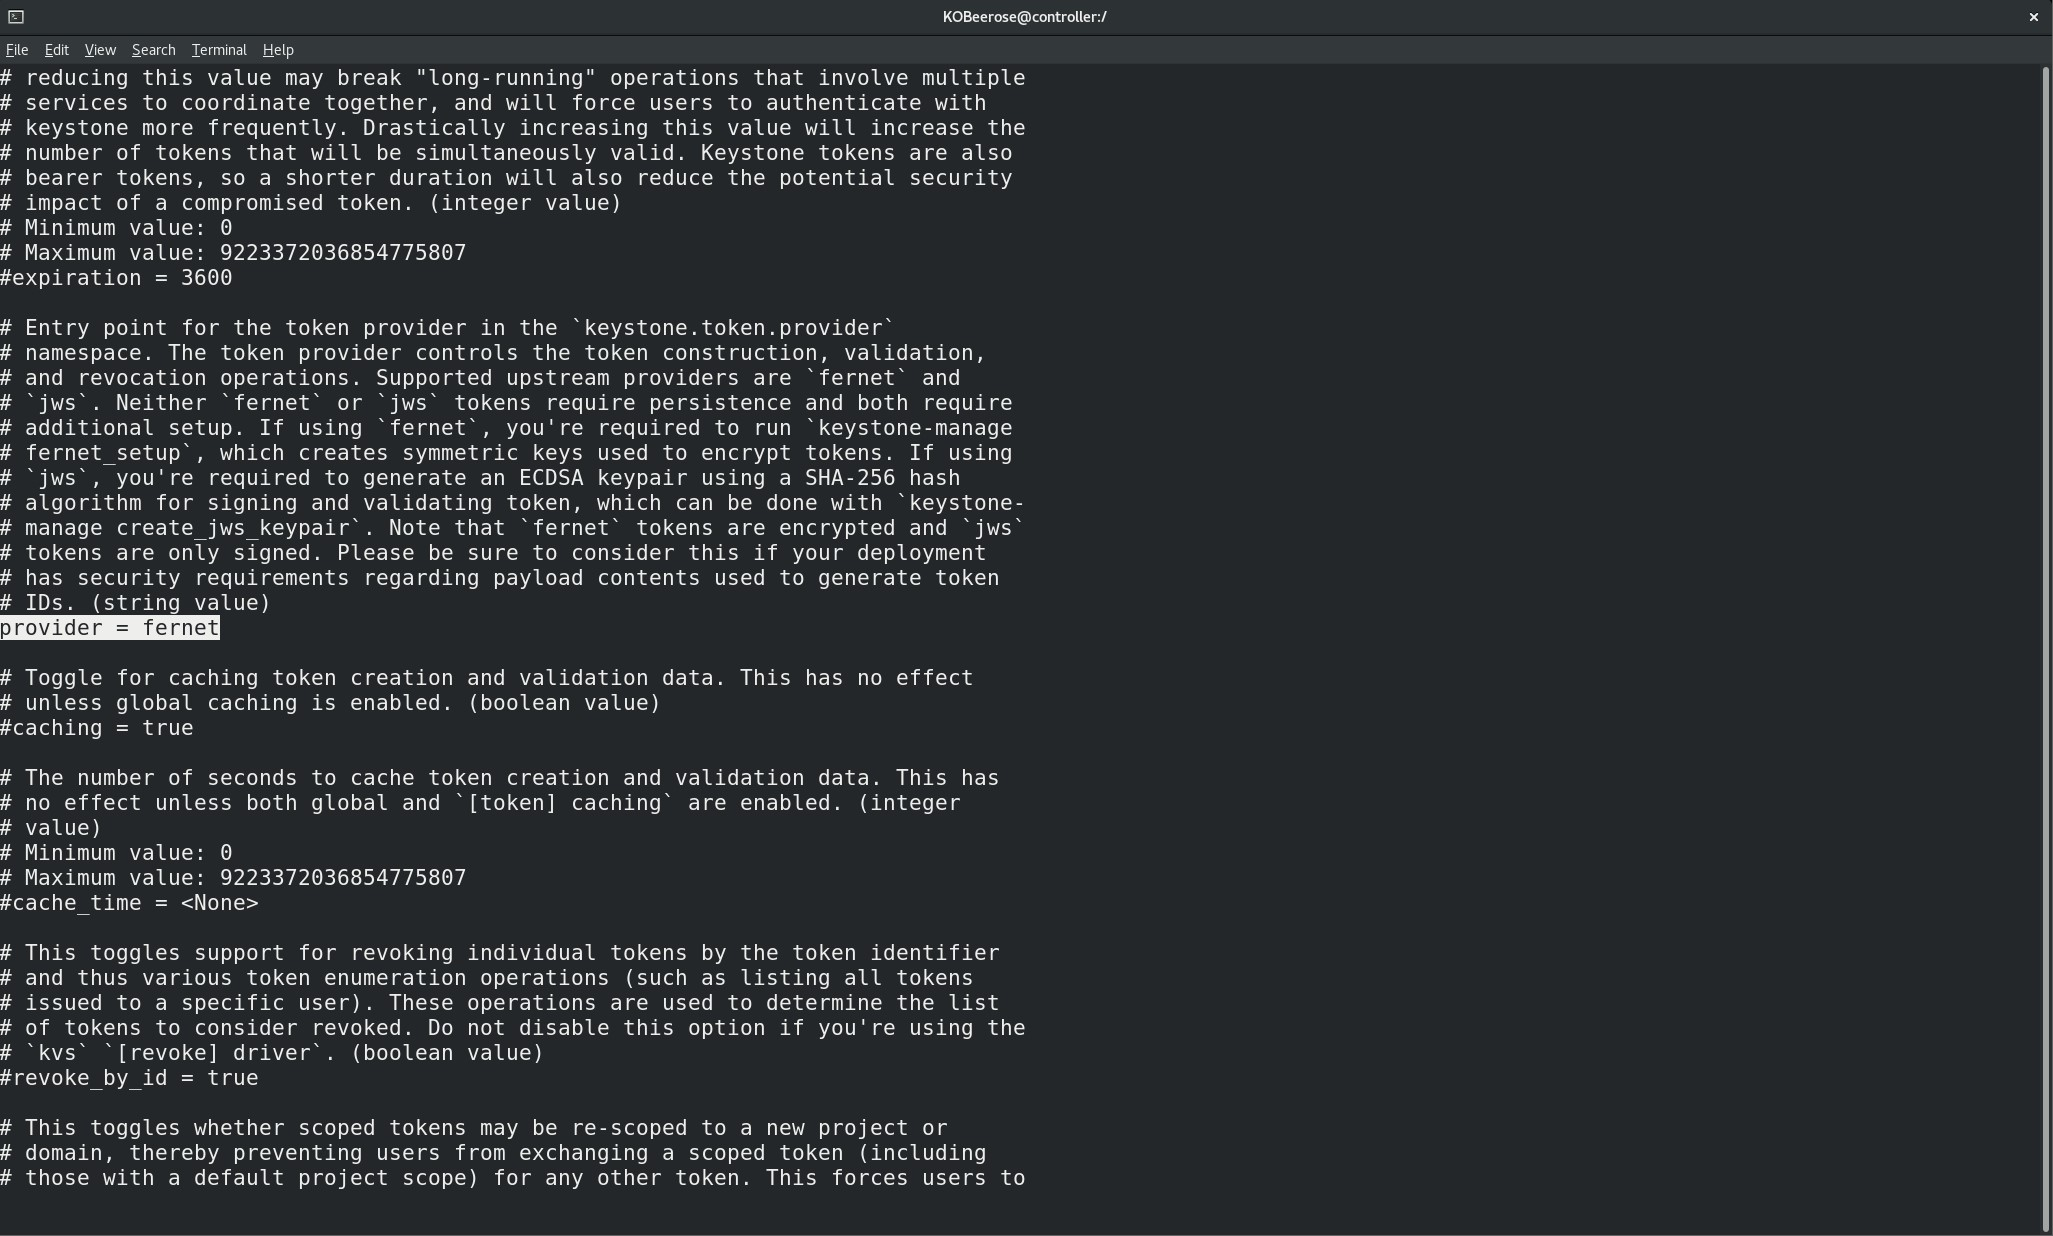
\includegraphics[width=1\linewidth]{Cloud/Configure Keystone #1/keystone.conf file} 
\end{center} 
\caption{keystone.conf file} 
\end{figure}  \FloatBarrier
\\
\par After having synchronized Keystone, we will initialize the keys, define Keystone Host and
run the keystone-manage bootstrap command to create a user, project, and role, and
assign roles. By default, the names of these new resources will be called admin. 
\\
\begin{figure}[!htb] 
\begin{center} 
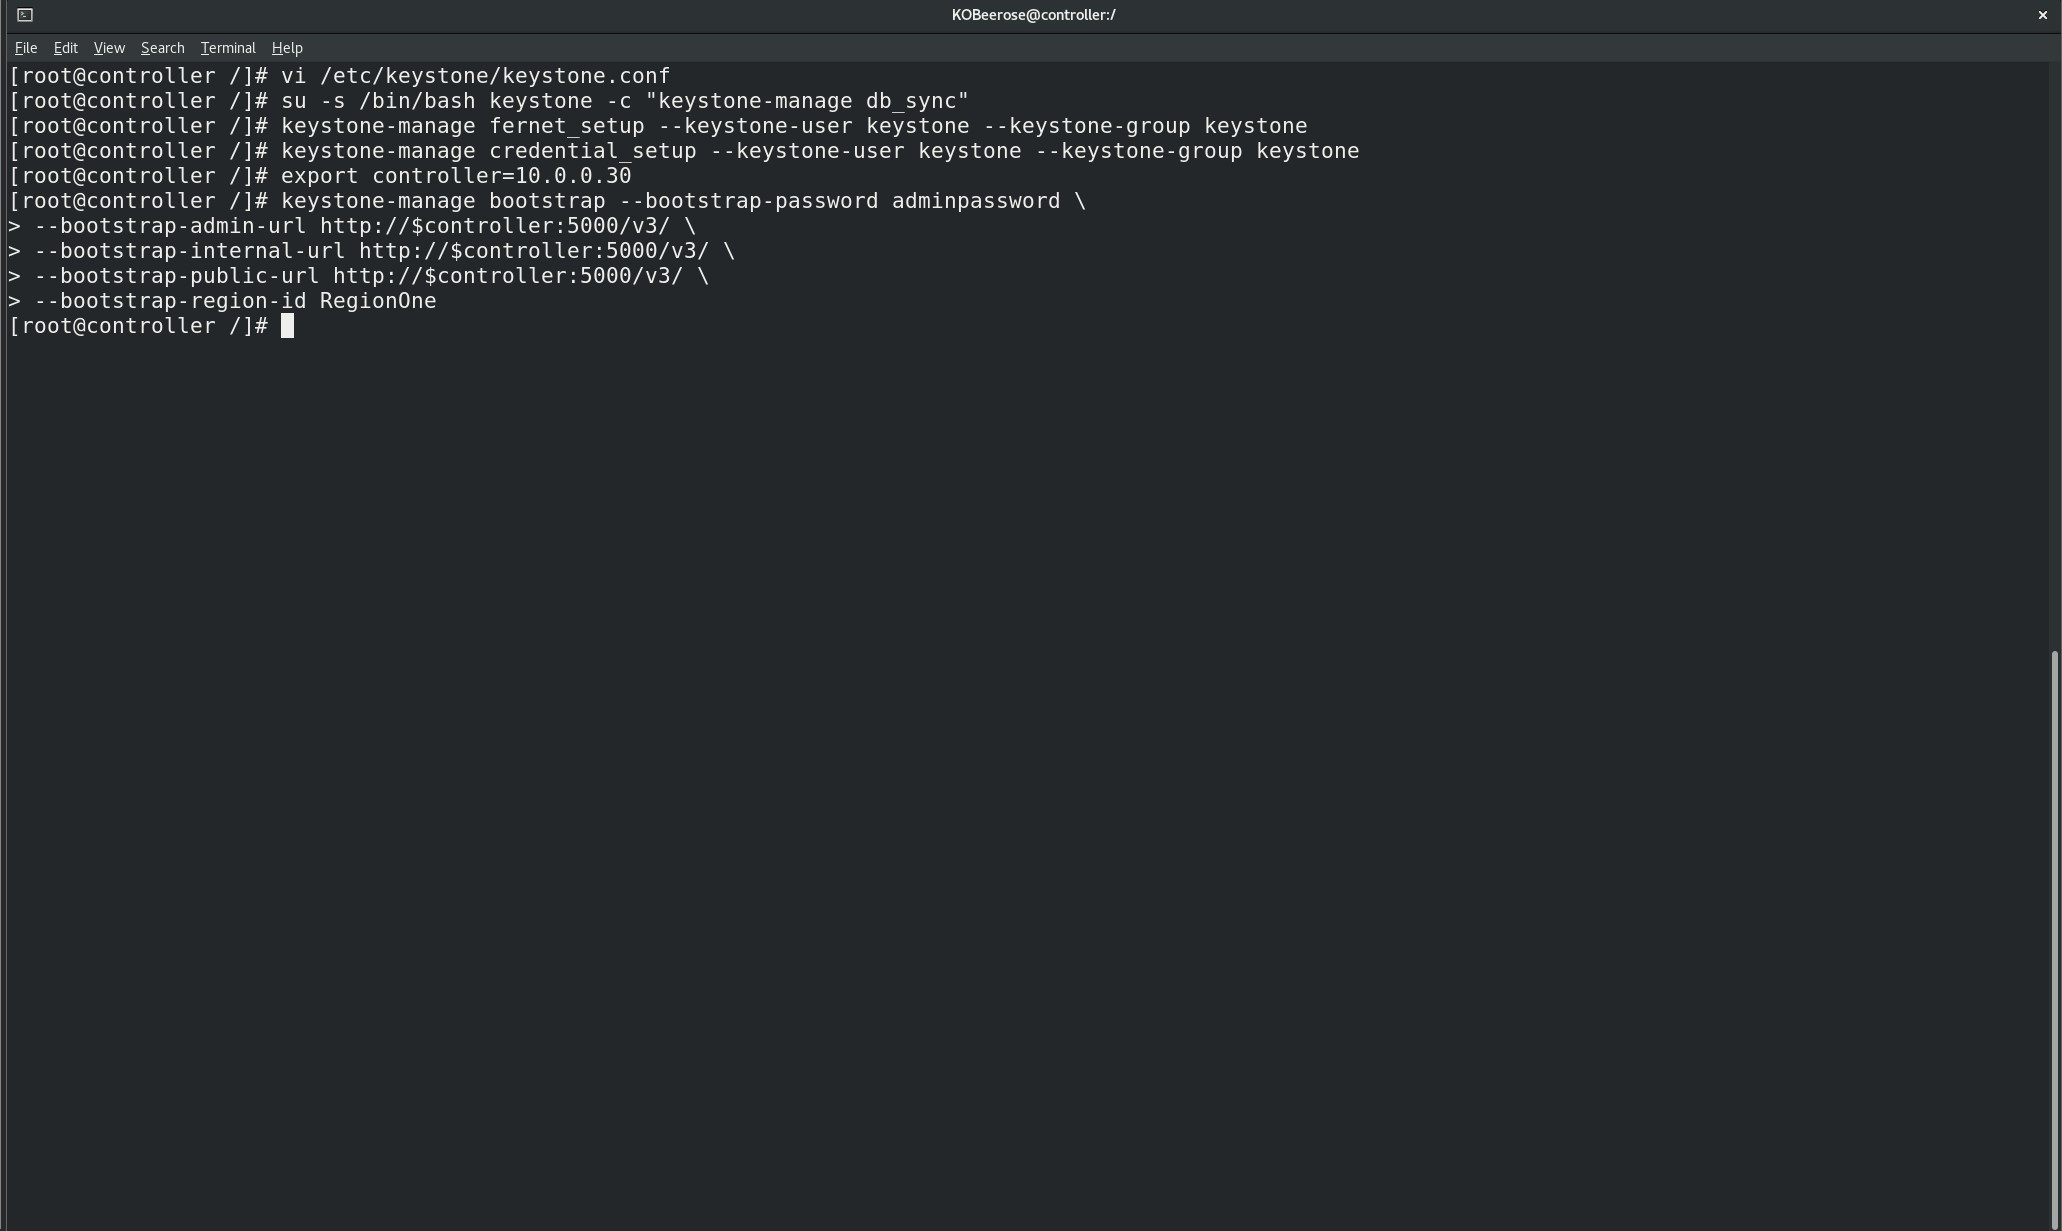
\includegraphics[width=1\linewidth]{Cloud/Configure Keystone #1/Configure Keystone} 
\end{center} 
\caption{Configure Keystone} 
\end{figure}  \FloatBarrier
\\
\section{keystone-httpd config}
\par 
As always, we need to change the boolean parameters of selinux and change the policy by creating a new module keystone-httpd.te to compile as shown below
\\
\begin{figure}[!htb] 
\begin{center} 
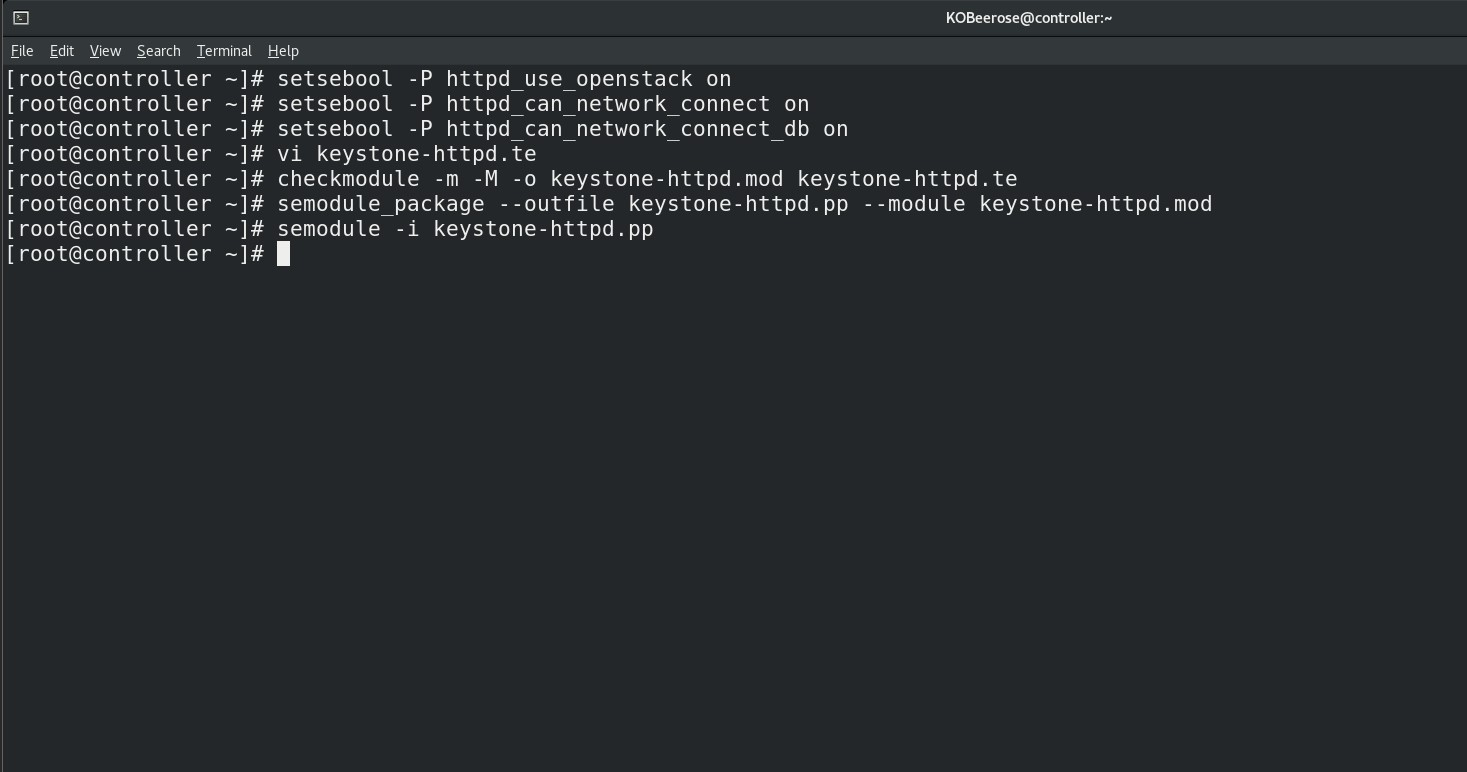
\includegraphics[width=1\linewidth]{Cloud/Configure Keystone #1/keystone-httpd config} 
\end{center} 
\caption{keystone-httpd config} 
\end{figure}  \FloatBarrier
\\
\section{Starting Apache httpd}
\par 
First step is allowing the port 5000 service and reloading the firewall.
\\
\begin{figure}[!htb] 
\begin{center} 
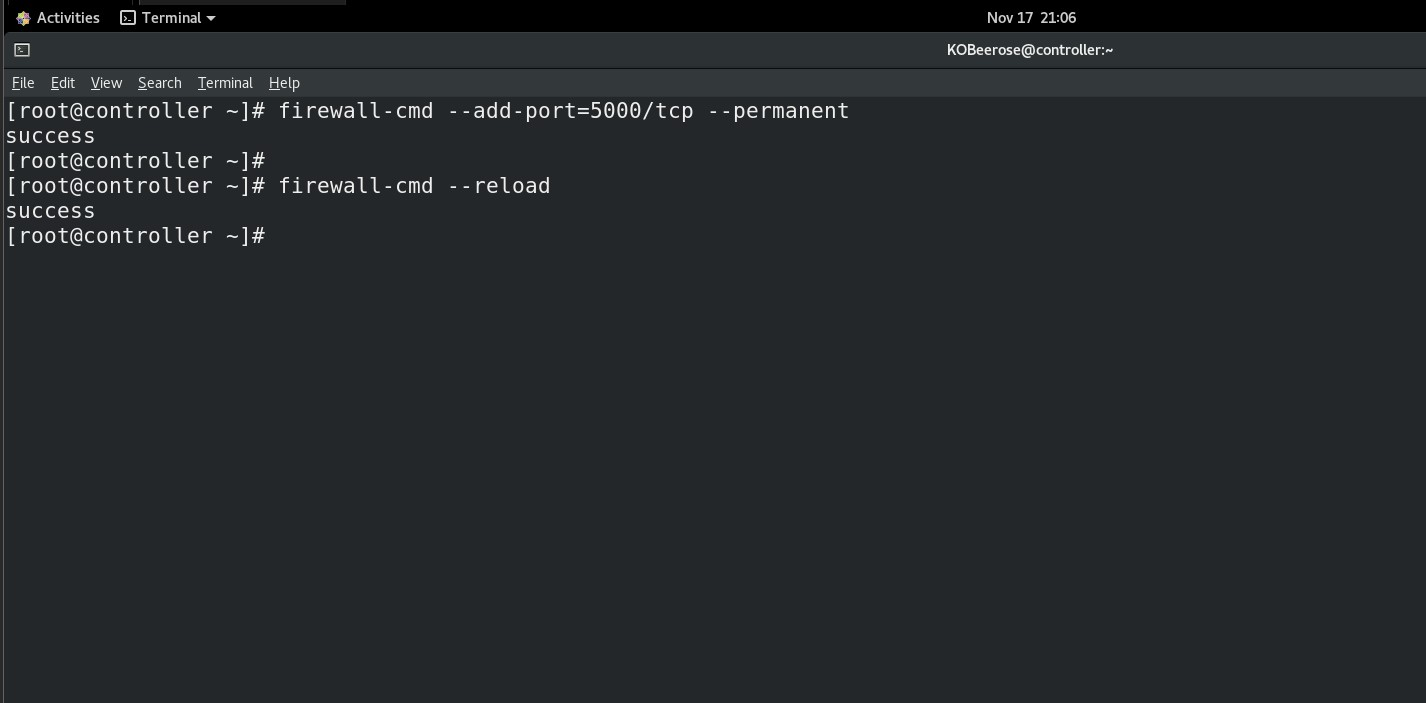
\includegraphics[width=1\linewidth]{Cloud/Configure Keystone #1/Allowing 5000 port} 
\end{center} 
\caption{Allowing 5000 port} 
\end{figure}  \FloatBarrier
\\
\par 
Once everything is configured, we will modify the /etc/httpd/conf/httpd.conf file to set the server name, then start Apache httpd. 
\\
\begin{figure}[!htb] 
\begin{center} 
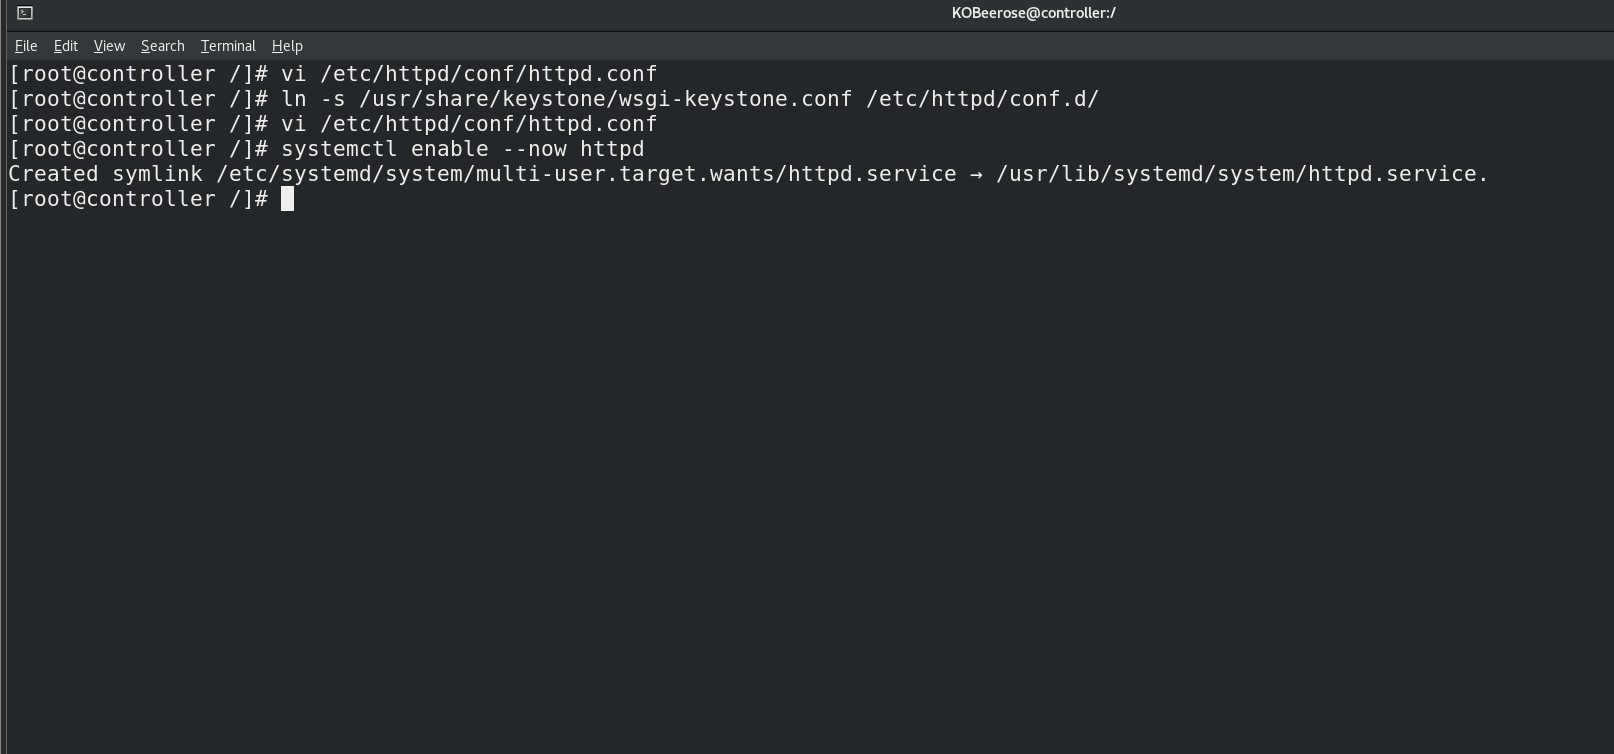
\includegraphics[width=1\linewidth]{Cloud/Configure Keystone #1/Apache httpd} 
\end{center} 
\caption{Apache httpd} 
\end{figure}  \FloatBarrier
\\
\section{Creating and Load environment variables file}

\par One more step before creating keystone projects, we are going to export some environment variables written in the  / keystonerc file as shown below: 
\begin{figure}[!htb] 
\begin{center} 
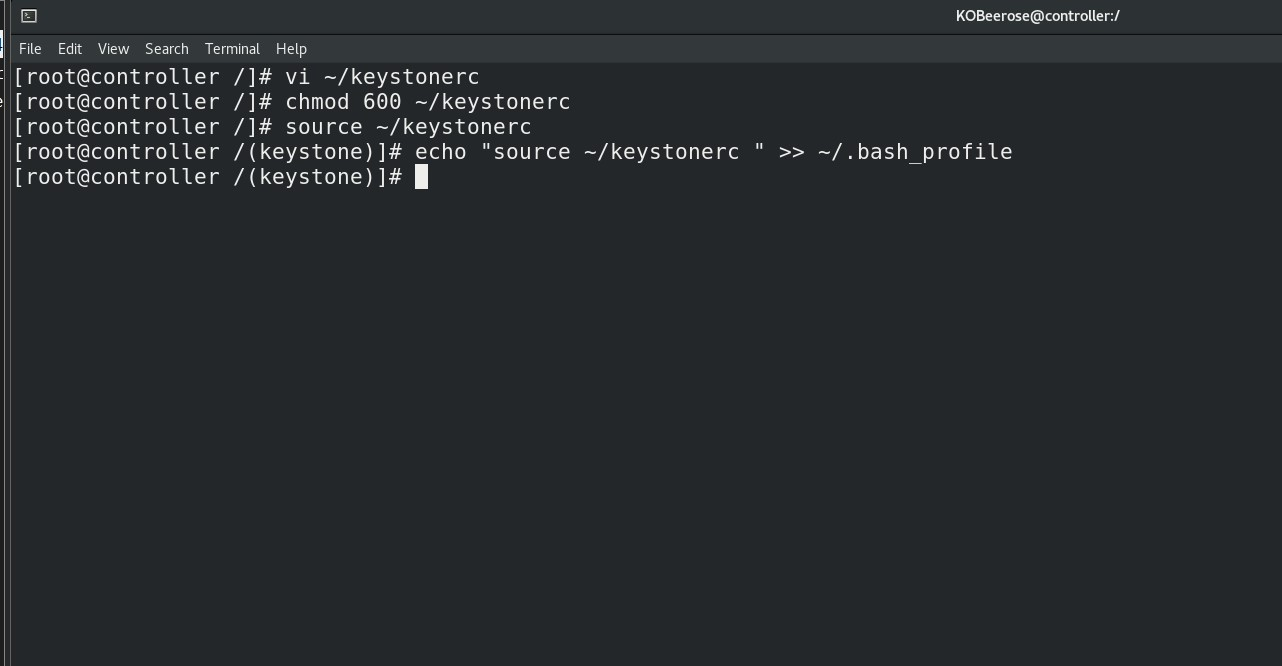
\includegraphics[width=0.94\linewidth]{Cloud/Configure Keystone #2/Creating env var file} 
\end{center} 
\caption{Creating env var file} 
\end{figure}  \FloatBarrier

\section{Creating Projects}

\par Finally, we can create a service project named service. to check it, we can display all the created projects 

\begin{figure}[!htb] 
\begin{center} 
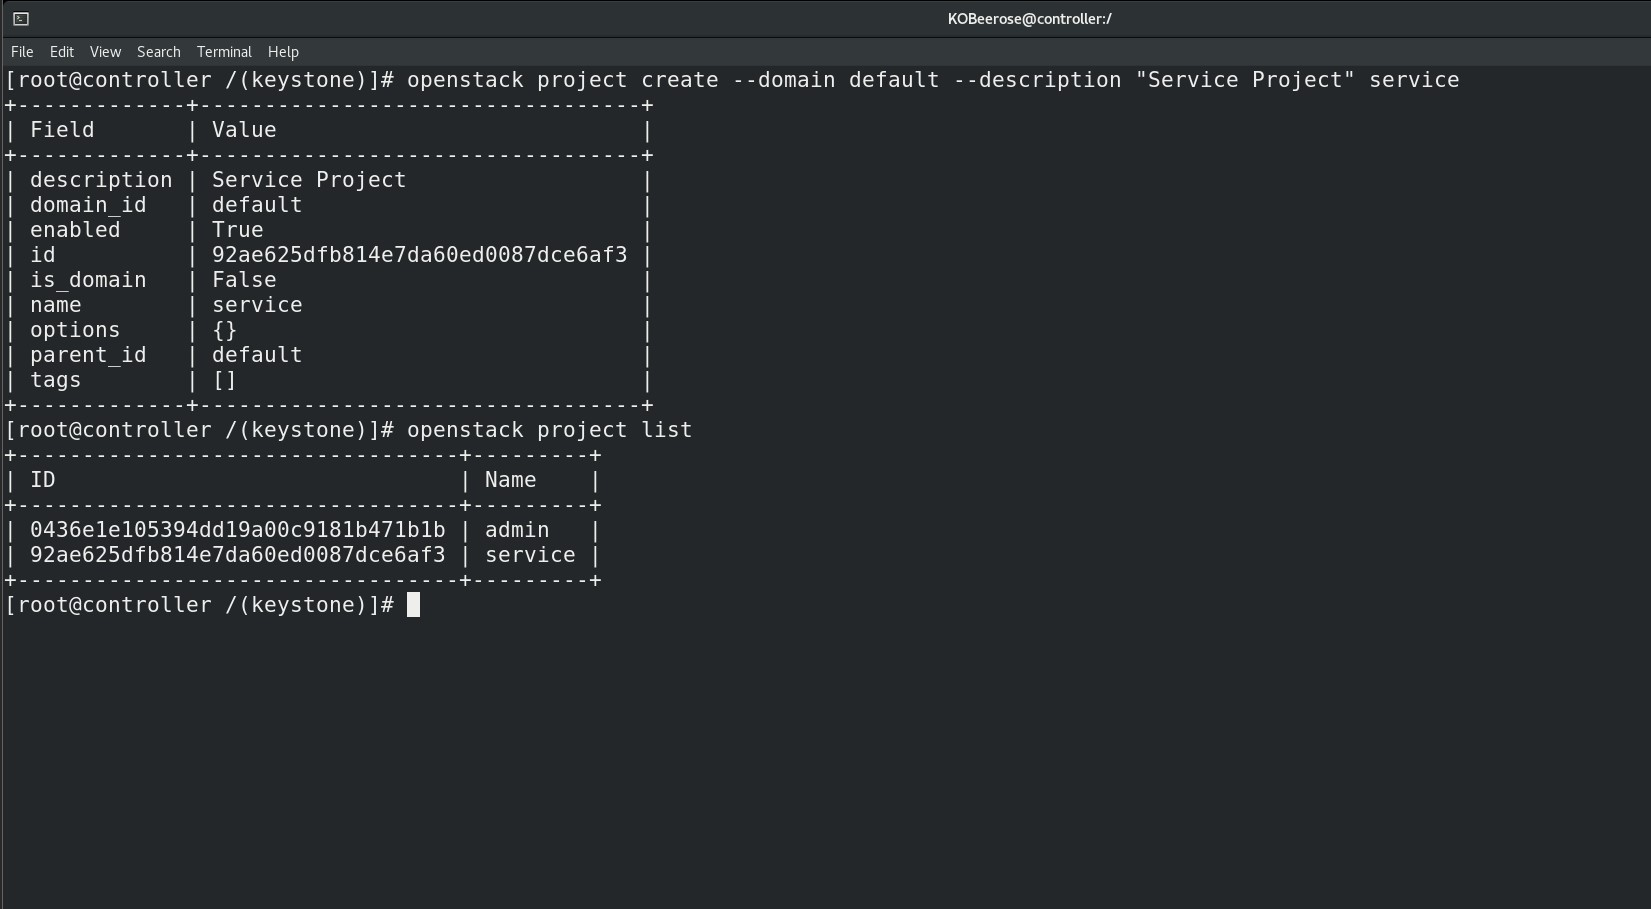
\includegraphics[width=.94\linewidth]{Cloud/Configure Keystone #2/Create Project} 
\end{center} 
\caption{Create Project} 
\end{figure}  \FloatBarrier
\\

\end{spacing}

\chapter{Running Map/Reduce in a multi-node cluster}
\par In this section we will running a Map / Reduce program in a multi-node cluster.
%Intro\footnotemark\\
\begin{spacing}{1.2}
%note en bas de page
\section{Checking all the nodes of the cluster}

\par Let's verify the good functioning of all the nodes of the cluster.
\\
\begin{figure}[!htb] 
\begin{center} 
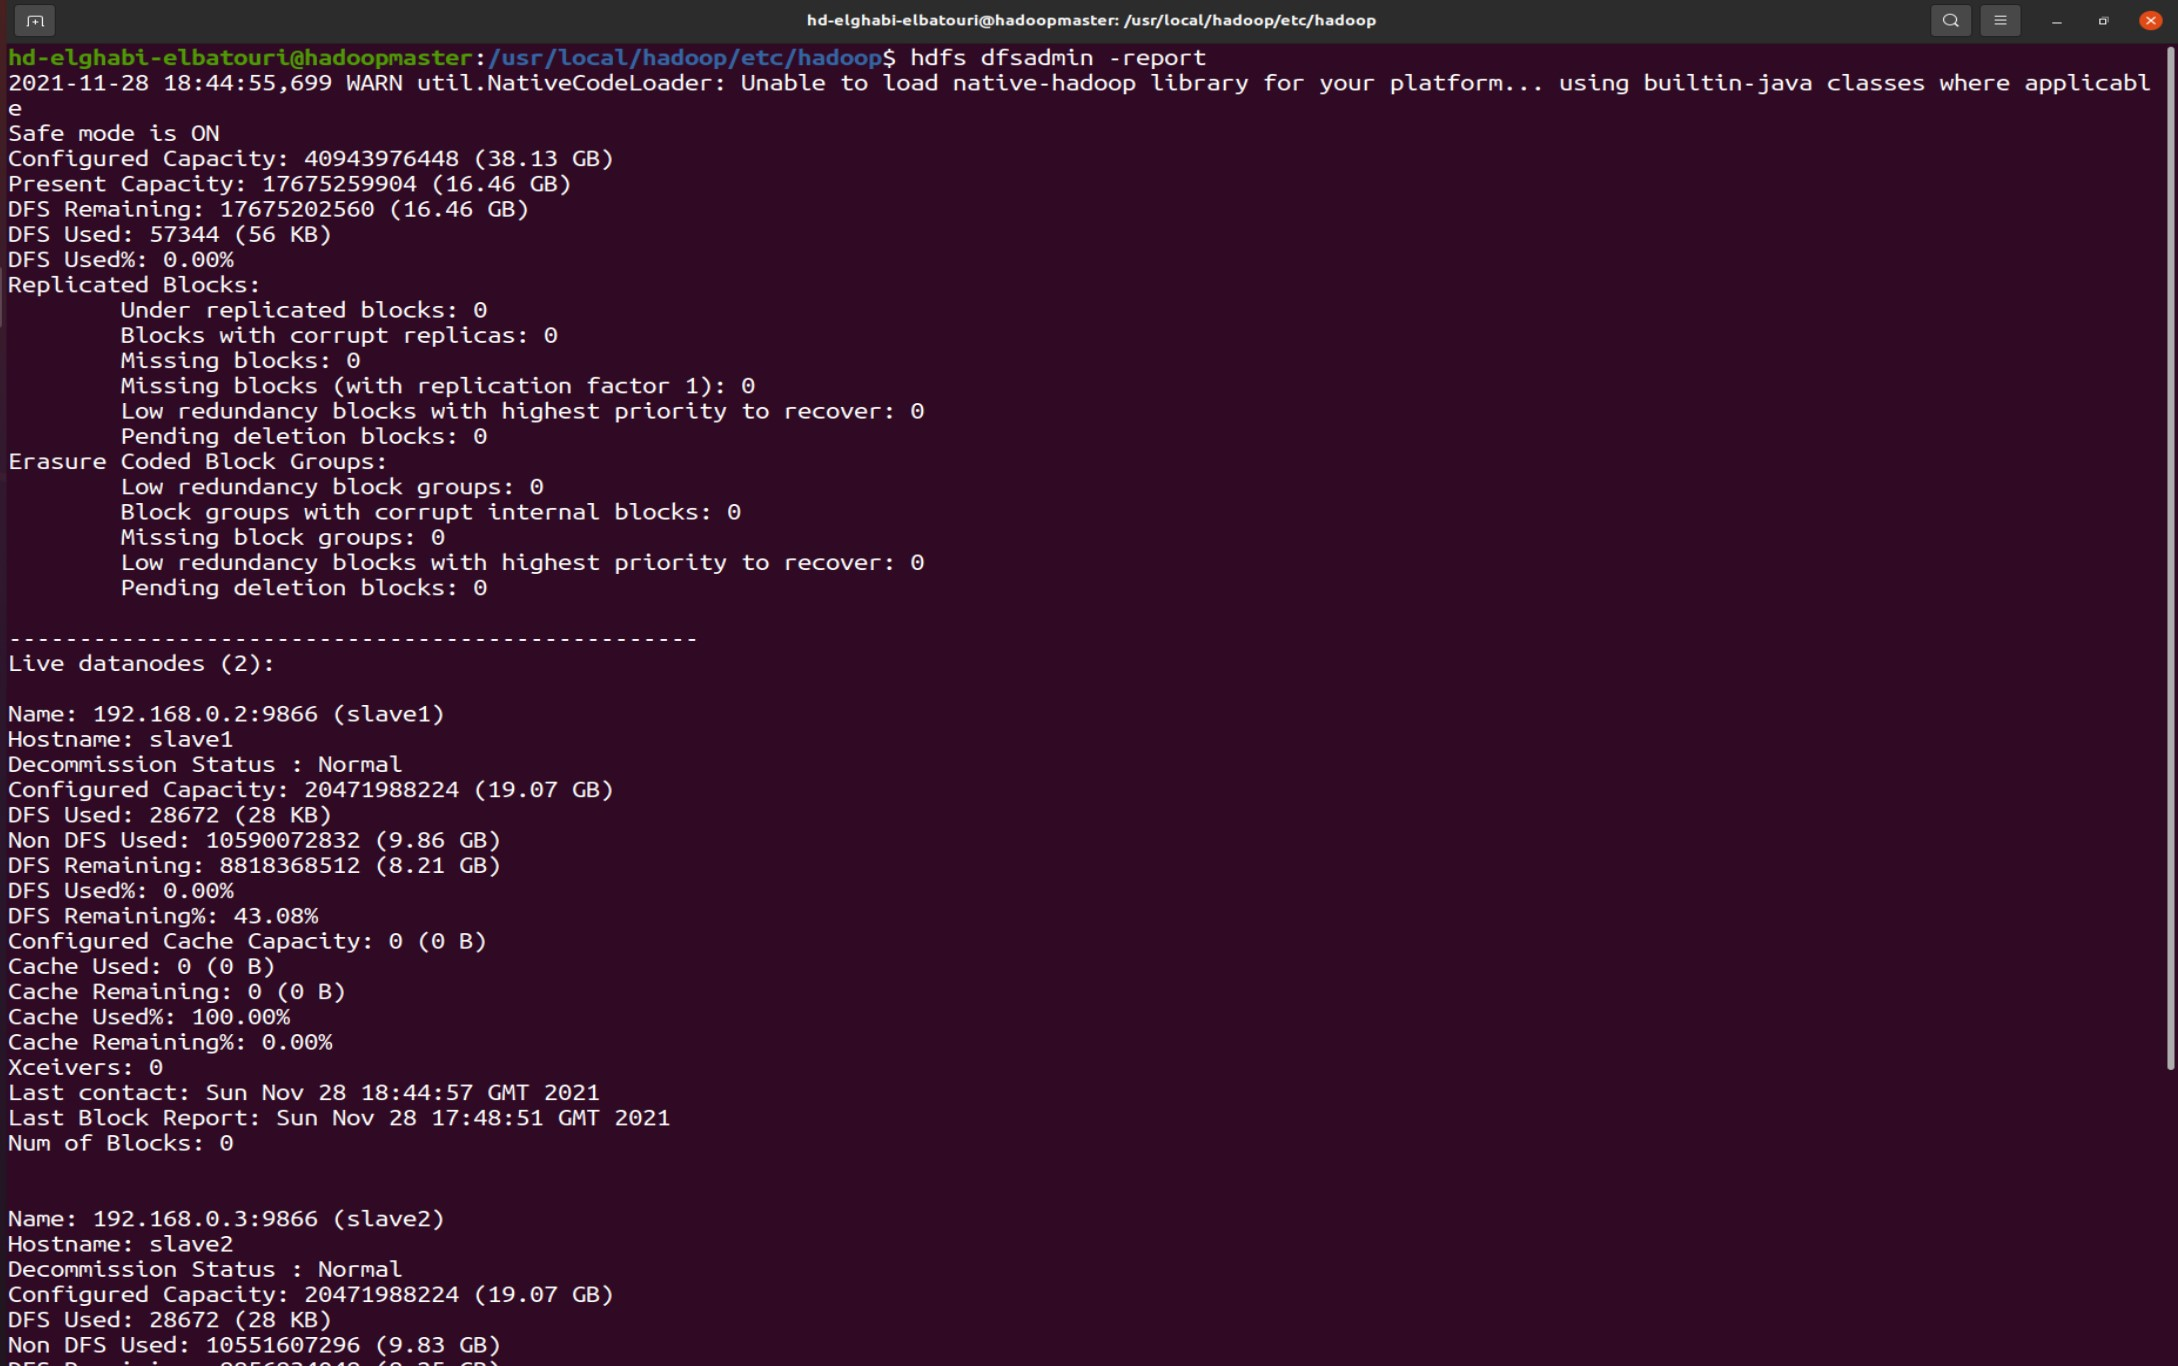
\includegraphics[width=1\linewidth]{Big_Data/Hadoop/Multi-Nodes Map_Reduce/Verifying cluster nodes.jpg} 
\end{center} 
\caption{caption} 
\end{figure} 
\FloatBarrier



\section{Executing Map/Reduce}

\par thisIsAveryLongParagraphToUseAsAtemplateForCopyAndPastingContentInAgoodWay
\\
\begin{figure}[!htb] 
\begin{center} 
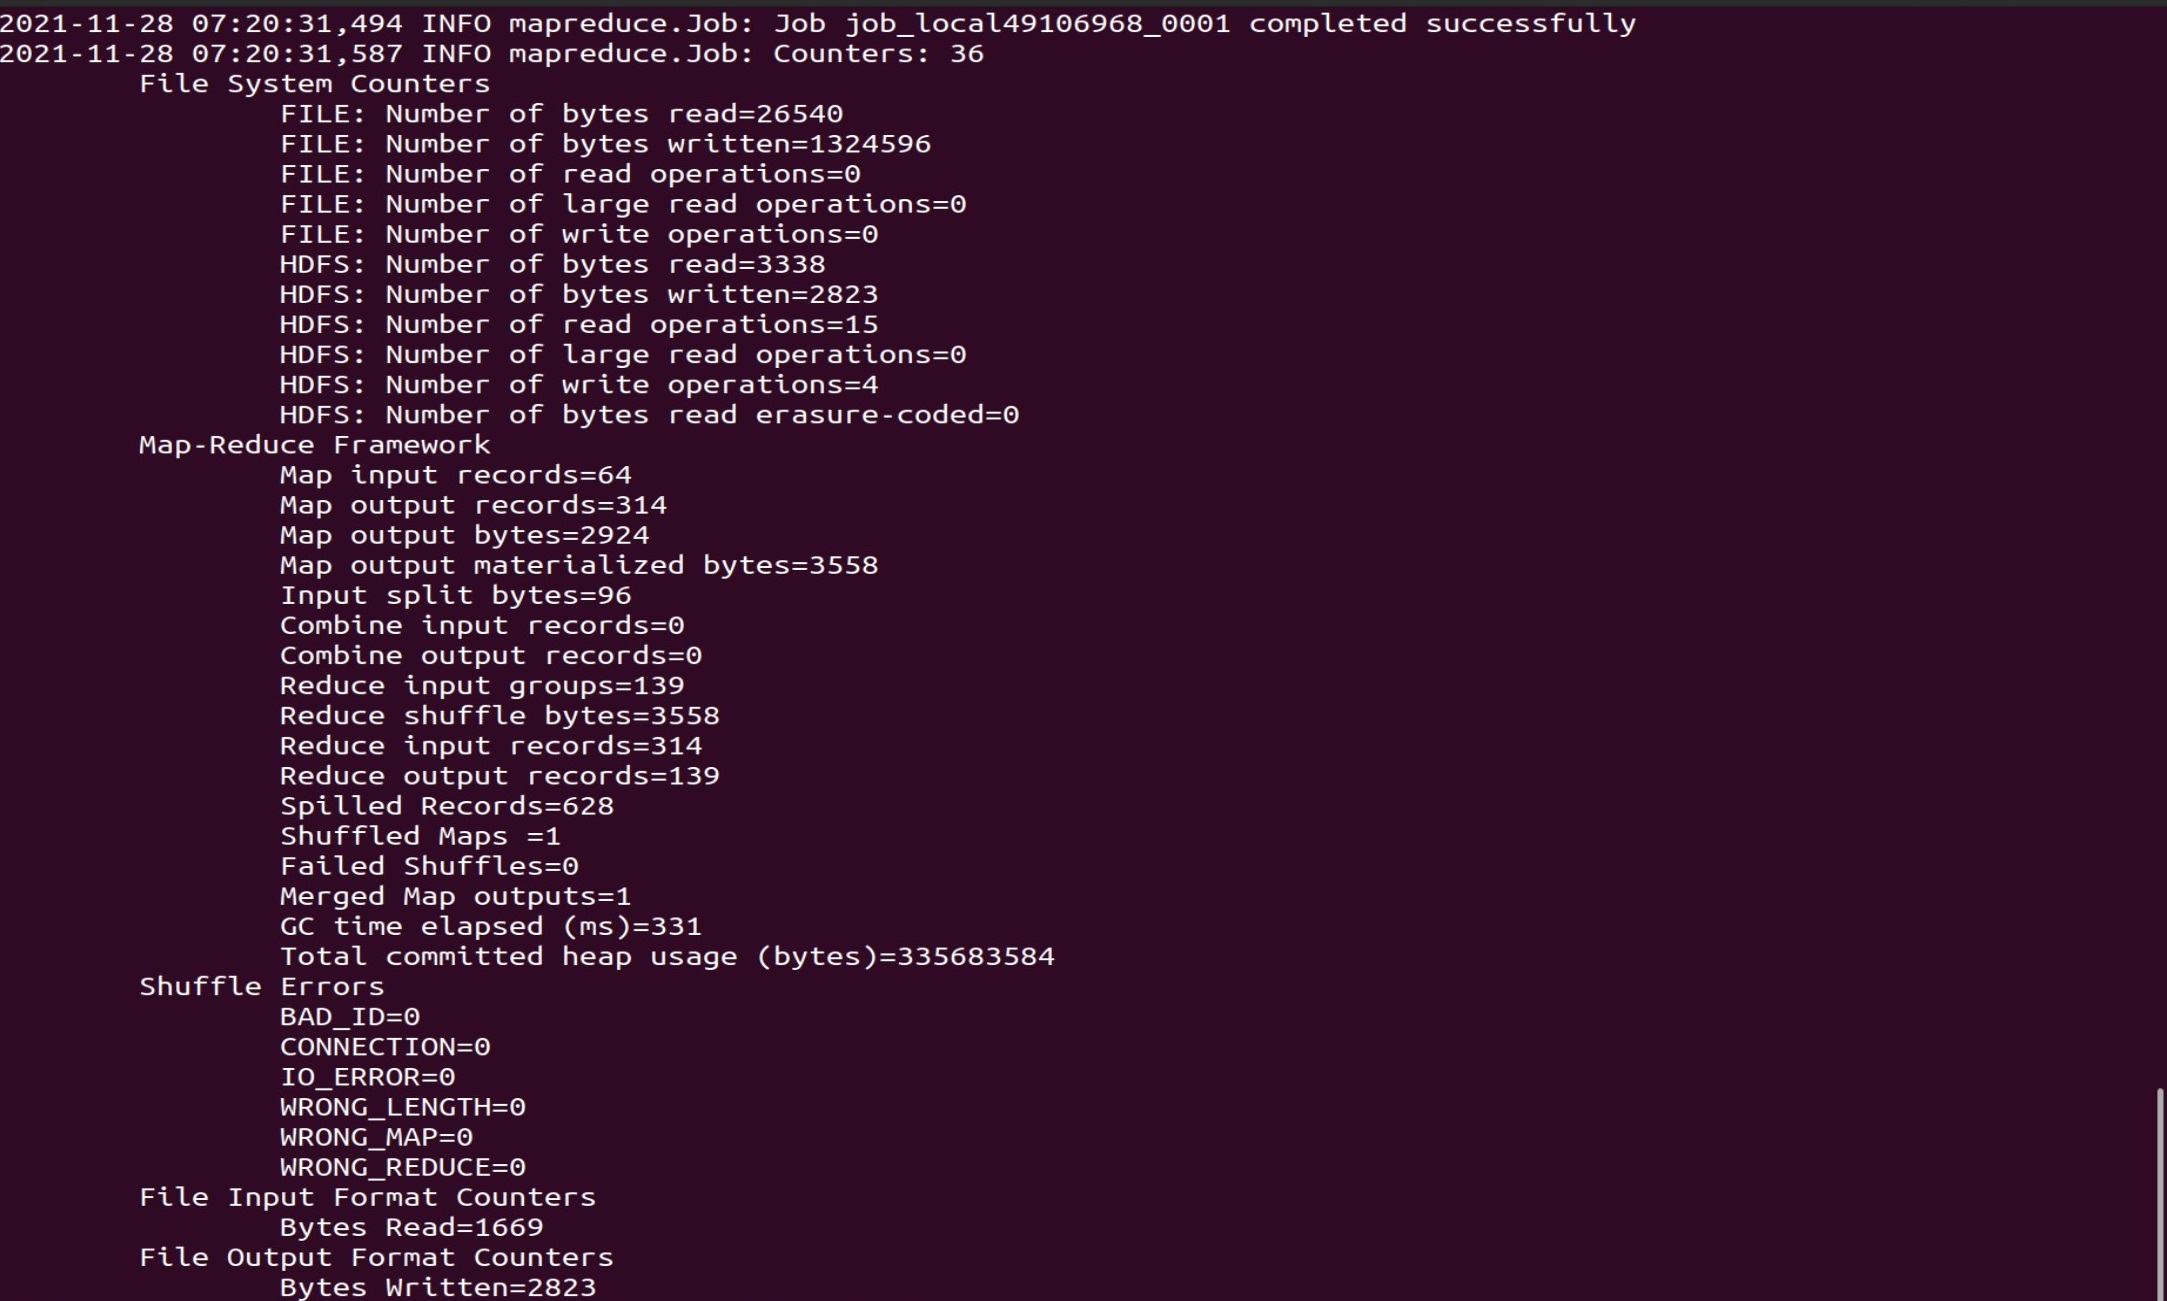
\includegraphics[width=1\linewidth]{Big_Data/Hadoop/Multi-Nodes Map_Reduce/running wordcount.jpg} 
\end{center} 
\caption{caption} 
\end{figure} 
\FloatBarrier


\section{Showing results}

\par Getting the result of the Map / Reduce algorithm.
\\
\begin{figure}[!htb] 
\begin{center} 
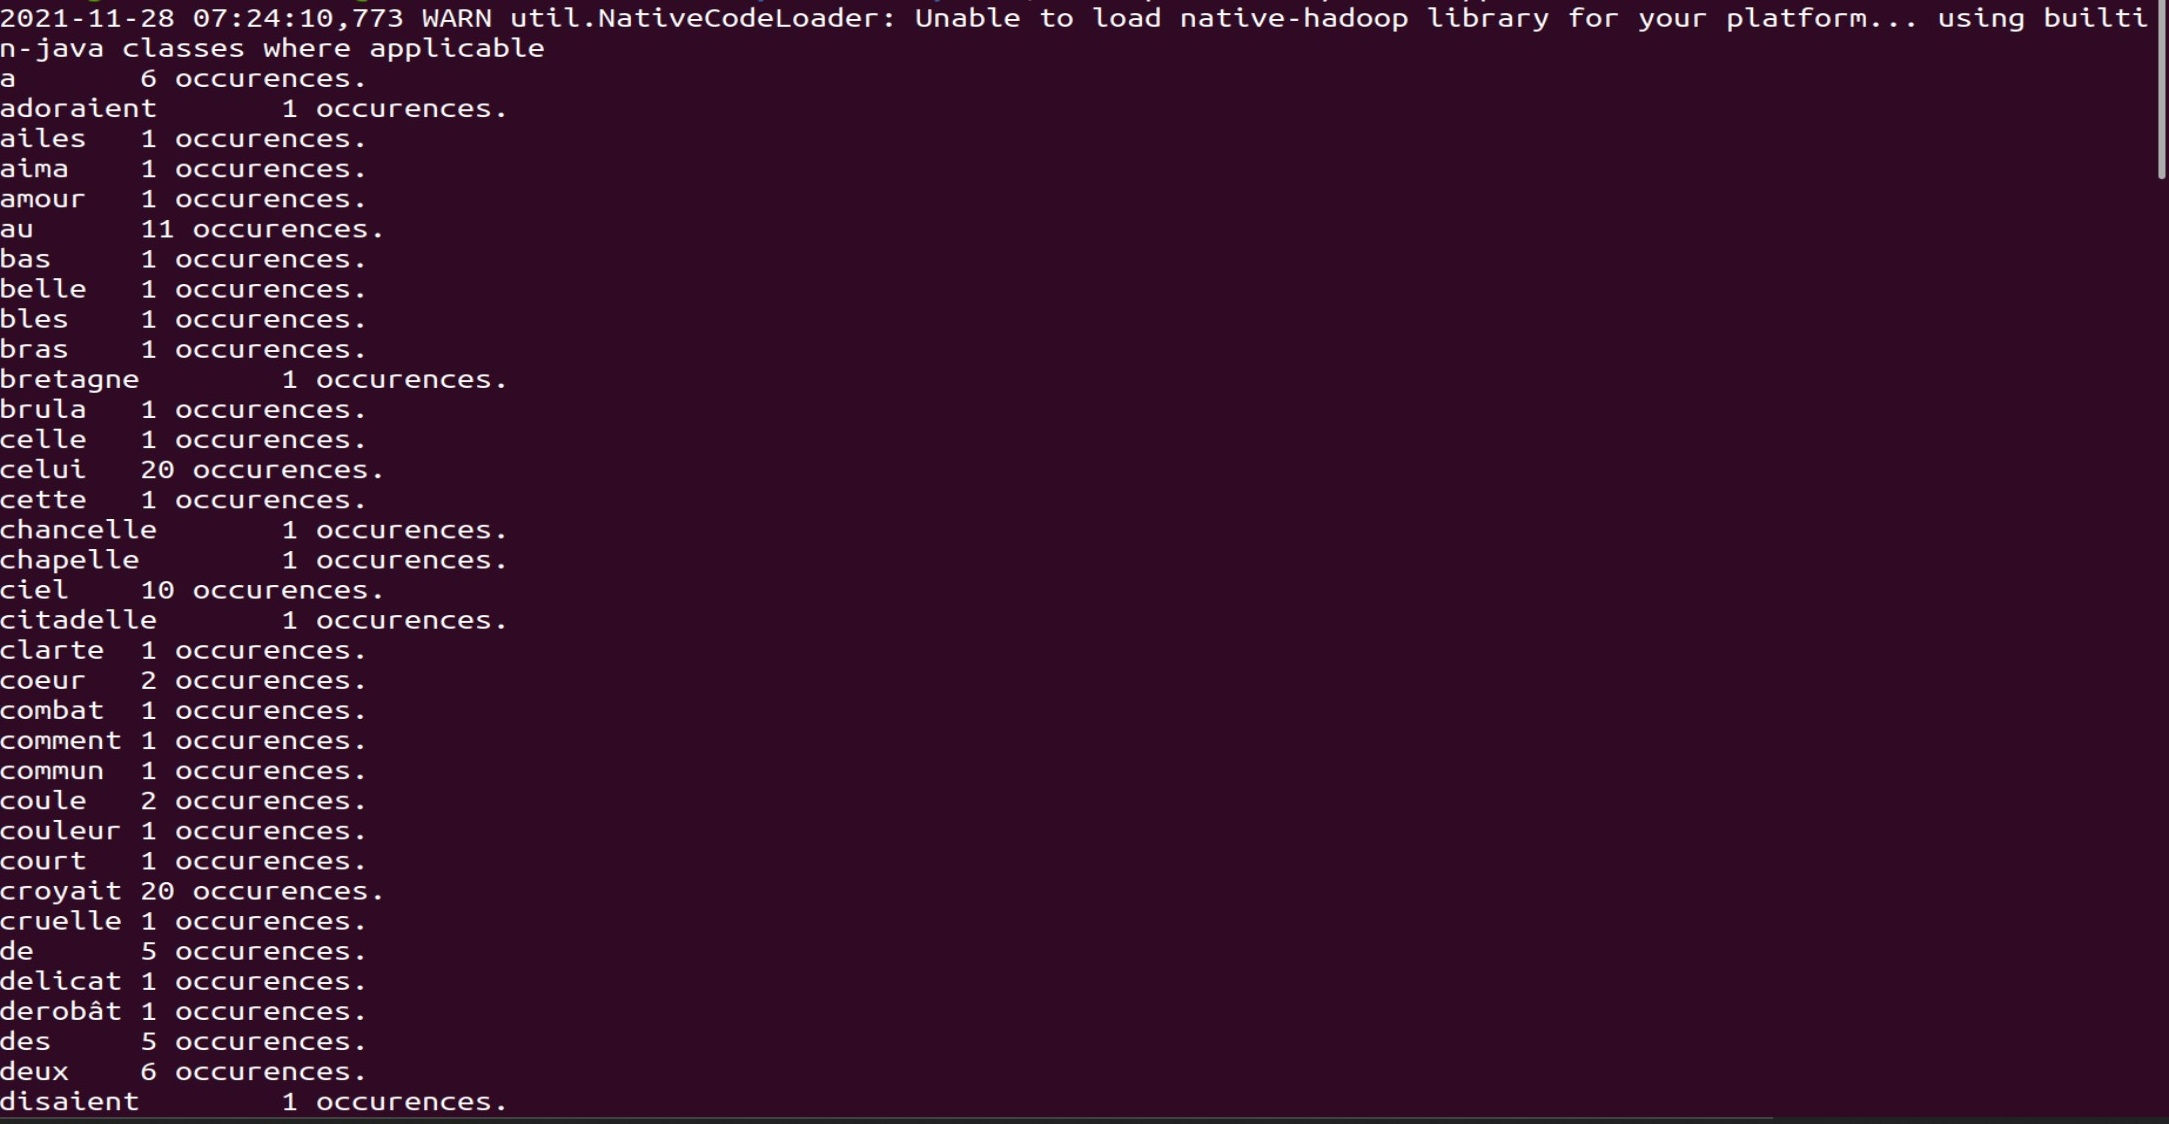
\includegraphics[width=1\linewidth]{Big_Data/Hadoop/Multi-Nodes Map_Reduce/Showing results.jpg} 
\end{center} 
\caption{caption} 
\end{figure} 
\FloatBarrier


\end{spacing}

%Ne pas numéroter cette partie
%\part*{Annexes}
%Rajouter la ligne "Annexes" dans le sommaire
\addcontentsline{toc}{part}{Conclusion}
\chapter*{Conclusion}
% \newpage
\vspace{1cm}
\par \Large 
In conclusion, we tried in this humble project to make a basic version of an application using multiple technologies. The objective of this project is ultimately to create a Log Visualiser with Spark streaming, Elasticsearch, Kibana and Kafka.  \\
\par \Large To accomplish this we have carried out several steps including: 
\begin{flushleft} \large
{
\item \textbf{-Deciding the Project Architecture,} \\[0.7cm]
\item \textbf{-Making a version with a first method: data source reading from files,}\\[0.7cm]
\item \textbf{-Second method using Kafka for streaming,}\\[0.7cm]
\item \textbf{And finally, we finished with the Configuration and use cases of Kibana.}
\item
}
\end{flushleft}

A project which aims to inject the data from the logs with Spark Streaming and to restore the result in the form of a dashboard under Kibana, which makes it easier to view and analyze the contents of the log files, this information can give us information on the profile of the user through his preferences and the sites he frequents the most. We can through this information and with the help of deep-learning algorithms make targeted advertising (it is the idea of a new project which will complete this one and which will be more useful).
\\\\
It was a pleasant and enjoyable project in which we acquired a lot of knowledge and skills.
We thank our dear supervisor, Mr.ZIYATI Houssaine, for these efforts and for the next adventure.

\newpage
%\addcontentsline{toc}{part}{Webography}
%\chapter*{Webography}

\vspace{2cm}

\begin{itemize}

\\\item \textbf{\Large{Kaggle.com : }}\\
\\{[1]} source de la dataset [\url{https://kaggle.com}] \vspace{0.3cm}

\\\item \textbf{\Large{OneVsRestClassifier : }}\\
\\{[2]} Fonction de classification pour notre modèle [\url{https://scikit-learn.org/stable/modules/generated/sklearn.multiclass.OneVsRestClassifier.html}] \vspace{0.3cm}

\\\item \textbf{\Large{Cours et documentations : }}\\
\\{[3]} Android O & Java - The Complete Android Development Bootcamp  [\url{https://www.udemy.com/course/android-app-development-with-java/}] \vspace{0.3cm}

\\{[4]} HeadFirst JAVA, auteurs : Bert Bates et Kathy Sierra 
\vspace{0.3cm}
\\{[5]} Documentation Android Studio :[ \url{https://developer.android.com/guide/}]
\vspace{0.3cm}
\\{[6]} Documentation Firebase :[ \url{https://firebase.google.com/docs/android/setup}]
\vspace{0.3cm}
\\{[7]} Documentation GoogleMaps : [ \url{https://developers.google.com/maps/documentation/android-sdk/map}]
\vspace{1cm}

\\ \item \textbf{\Large{Forums et Siteweb:}}\\
\\{[6]} Stackoverflow [\url{http://www.stackoverflow.com}]
\vspace{0.3cm}
\\{[7]} Medium [\url{https://medium.com}]

\vspace{1cm}
\\ \item \textbf{\Large{Chaînes Youtube :}}\\
\\{[8]} Firebase 
[\url{https://www.youtube.com/channel/UCP4bf6IHJJQehibu6ai__cg}]
\vspace{0.3cm}
\\{[9]} CodingWithMitch [\url{https://www.youtube.com/channel/UCoNZZLhPuuRteu02rh7bzsw}]\\
\\{[10]} Coding in Flow [\url{https://www.youtube.com/channel/UC_Fh8kvtkVPkeihBs42jGcA}]

\end{itemize}



%récupérer les citation avec "/footnotemark"
\newpage
\nocite{*}
\bibliographystyle{unsrt}
%inclusion de la biblio
\bibliography{biblio.bib}
\addcontentsline{toc}{chapter}{Bibliography}

\end{document}